\documentclass[a4paper, 11pt, titlepage, twoside]{article}

\usepackage{preamble}

\begin{document}
%Canviem el nom de l'apartat Referències per ``Bibliografia''

%Portada

%%CANVIEU L'ESPAI VERTICAL ENTRE ELEMENTS SEGONS LA LLARGADA DEL TÍTOL
\begin{titlepage}
    {\centering
    {\Huge Master Thesis}\\
    \vspace{5mm}
    {\Large \textbf{Double MSc Degree in Industrial Engineering and Energy Engineering}}\\
    \vspace{20mm}
    \Huge \textbf{Dynamic Simulation and Stability Analysis of Power Systems: Development of RMS and EMT Tools within VeraGrid at eRoots}\\
    \vspace{10mm}
    \Large{January 2026}\\  %Data de la darrera complicació, si voleu posar una data fixa, escriviu-la aquí
    }
    \vspace{25mm}
    \hspace{2mm}
    \begin{tabular}{l@{ } l}
        \vspace{5mm}
        \Large \textbf{Author:} & \hspace{3mm} \Large{Maria Sans Esqué} \\
        \vspace{5mm}
    \Large\textbf{Supervisors:} & \hspace{3mm} \Large{Vinícius Albernaz Lacerda} \\
                                & \hspace{3mm} \Large{Josep Fanals i Batllori} \\

    \end{tabular}\par
    \vspace{10mm}
    {\centering
    
\includegraphics[scale=0.3]{./Icones-ETSEIB-UPC/ETSEIB.png}\\
    {\Large Escola Tècnica Superior \\ d'Enginyeria Industrial de Barcelona}\\
    \vspace{3mm}
    
\includegraphics[scale=0.4]{./Icones-ETSEIB-UPC/UPC.PNG}
    \par
    }
    \end{titlepage}

%Pàgina en blanc
\clearpage
\thispagestyle{empty}
\null\newpage 

%iniciem la numeració des del Resum
\pagenumbering{arabic}

\section*{Abstract}\label{Abstract}
\input{Chapters/Abstract}
\cleardoublepage
\section*{Resumen}\label{Resumen}


\cleardoublepage
\section*{Resum}\label{Resum}





\cleardoublepage

\tableofcontents

\newpage
\listoffigures

\newpage
\begingroup
\setlength{\parskip}{0pt}
\listoftables %Opcional
\endgroup

\setlength{\abovedisplayskip}{5pt} % Equation spacing adjusted
\setlength{\belowdisplayskip}{5pt} % Equation spacing adjusted

\section*{Glossary}
\addcontentsline{toc}{section}{Glossary}
\subsection*{Symbols}
\begin{tabular}{l@{\hspace{1.95cm}} l}
  $\bm{\theta}$ & Voltage angle vector \\
  $\lambda$ & Eigenvalue \\
  $\zeta$ & Damping ratio \\
  $\bm{\omega}$ & Angular frequency vector \\
  $\bm{A}$ & State matrix \\
  $\bm{B}$ & Input matrix \\
  $\bm{C}$ & Output matrix \\
  $\bm{D}$ & Feedthrough matrix \\
  $\bm{x}$ & State vector \\
  $\bm{u}$ & Input vector \\
  $\bm{y}$ & Output vector \\
  $\tau$ & Time constant \\
  
  
 
\end{tabular}


\subsection*{Acronyms}
\begin{tabular}{l@{\hspace{1cm}} l}
  AC & Alternating Current \\
  CIG & Converter-interfaced Generation \\
  DAE & Differential Algebraic Equation\\
  DC & Direct Current \\
  EEA & European Environment Agency\\
  EMT & Electro Magnetic Transient\\
  ETSEIB & Escola Tècnica Superior d'Enginyeria Industrial de Barcelona\\
  GUI & Guided User Interface\\
  HVAC & Heating Ventilation and Air Conditioning \\
  IBR & Inverter-Based Resources \\
  ICAEN & Institut Català de l'Energia \\
  IGE & Induction Generator Effect\\
  LCA & Life Cycle Assessment \\
  ODE & Ordinary Differential Equation \\
  PF & Participation Factor\\
  PSCAD & Power Systems Computer Aided Design\\
  RMS & Root Mean Square\\
  SFA &Shifted Frequency Analysis\\
  SPT & Singular Perturbation Theory\\
  SSCI & Subsynchronous Control Interaction\\
  SSR & Subsynchronous Resonance\\
  TDS & Time Domain Simulation\\
  
\end{tabular}\par
\newpage

\section*{Preface}
\addcontentsline{toc}{section}{Preface}
\input{Chapters/Preface.tex}
\newpage

\section{Introduction}\label{Introduction}
%INTRODUCTION
\subsection{Motivation}

...

\subsection{Objectives}

This thesis is part of the ongoing development of the dynamic simulation framework, 
with a focus on extending its capabilities to include small-signal stability analysis and foundational electromagnetic transient (EMT) modeling. 
The work is carried out within the Veragrid environment, where new modules and methodologies are being implemented. 
The main goal is to equip Veragrid with advanced tools for studying the dynamic behavior of power systems, integrating symbolic modeling, numerical routines,
and graphical interfaces for analysis and visualization.

\subsubsection*{General Objectives}

To develop and validate advanced methodologies for dynamic simulation and stability analysis of power systems by incorporating small-signal stability techniques and foundational EMT modeling, fully integrated into the Veragrid environment.

\subsubsection*{Specific Objectives}

\begin{itemize}
    \item To develop the small-signal analysis module for RMS models, including the formulation and linearization of differential-algebraic equations at the operating point, the computation of eigenvalues and participation factors from the Jacobian matrix, and its integration into Veragrid’s graphical interface.
    \item To implement the foundational components for EMT simulation, modeling transmission lines and system elements in the abc domain, applying discretization techniques such as the Dommel algorithm and alternatives like the 2S-DIRK method, and validating the EMT solver using benchmark systems compared against commercial tools such as PSCAD.
    \item To extend symbolic system formulation to support custom models and control schemes, improving numerical routines, and ensuring consistent initialization of dynamic studies.
    \item To validate the developed methodologies through case studies, continuously comparing results with commercial tools to ensure model reliability and correctness.
\end{itemize}




\subsection{Scope}

This thesis is part of the ongoing development of Veragrid, a leading software platform for power system planning and simulation. 
The work focuses on improving dynamic simulation tools for modern grids, particularly in the context of small-signal stability and electromagnetic transient (EMT) modeling.
Over a nine-month period—from September 2025 to May 2026—the project aims to build essential components that support symbolic formulation, numerical validation,
and integration with existing simulation environments. 

The first major area of focus is the implementation of small-signal stability analysis using RMS-based state-space models.
This includes the computation of eigenvalues and participation factors, symbolic reduction of system equations,
and integration of these routines into the VeraGrid graphical interface.
The goal is to provide researchers and engineers with intuitive and accurate tools for identifying dominant modes and assessing system stability under varying conditions.

The second area involves the development of a foundational EMT solver in the abc domain. This includes modeling transmission lines and components,
implementing discretization techniques such as the Dommel algorithm and two-stage diagonally implicit Runge-Kutta (2S-DIRK) methods,
and benchmarking solver performance against commercial tools like PSCAD. Although the EMT module is not intended to be exhaustive,
it serves as a proof of concept for future expansion and integration.

All development is conducted in Python, with an emphasis on code quality, symbolic computation, and reproducibility.
The thesis also includes continuous benchmarking and validation using real-world data, including industrial cases.
Technical supervision is provided by the eRoots team, ensuring alignment with architectural standards and long-term project goals.

\subsection{Structure of the document}

llistar tot jeje

\subsection{State of the art}

sdfsfgsfd

\subsection{Veragrid}

VeraGrid is a comprehensive software platform for power system planning and simulation, developed to offer both technical accuracy and accessibility. 
It integrates a wide range of analytical and optimisation tools, covering everything from traditional steady-state analyses to advanced planning functions 
that address the challenges of modern electrical grids. Its capabilities include conventional studies such as power flow, short-circuit, and contingency analyses, 
as well as linear and non-linear optimisation modules used for operational decision-making and long-term investment assessment. Many of these functions are based on 
established industry standards, while others are the result of ongoing research and innovation, designed to push the boundaries of what is possible in open and high-performance 
grid modelling.

\begin{figure}
  \centering
  
\includegraphics[width=0.8\linewidth]{figures/VeraGrid_banner.png}
  \caption{VeraGrid banner. \textit{Source: VeraGrid documentation \cite{veragrid}.}}
  \label{fig:VeraGrid_banner}
\end{figure}

The development of VeraGrid began in 2015 with a clear objective: to create a robust programming library supported by a user-friendly interface. 
This pragmatic vision led to a unique ecosystem where reliability and simplicity coexist with scientific rigour. Over the years, the platform has evolved through a combination 
of commercial projects, academic collaborations, and internal research initiatives, ensuring that its algorithms and methods remain both practical and forward-looking. 
Some of its innovations emerged from the need to address real-world industrial requirements, while others stemmed from curiosity and the exploration of new computational paradigms.

VeraGrid serves a wide audience. For professionals, it provides transparent, efficient, and reproducible tools that enable detailed grid analysis and operational planning. 
For researchers, it represents an open and validated environment capable of integrating experimental algorithms and comparing methodologies. For educators and students, 
it offers a pedagogical platform that connects theoretical concepts with practical, industry-grade implementations. This versatility allows VeraGrid to act as a bridge between 
academia, industry, and future generations of engineers.

Beyond conventional functionalities, VeraGrid includes an extensive set of features designed for modern power systems. 
These include a multi-layered architecture for both usability and computational efficiency; an AC/DC generalised power flow engine that supports hybrid 
grids and converter-based systems; short-circuit and fault analysis modules that incorporate converter control logic; and a suite of optimal power flow, expansion planning, 
and investment analysis tools. The platform also integrates time-series simulation capabilities for renewable energy forecasting, storage operation, and market coupling, 
enabling comprehensive scenario-based studies. 

Thanks to its open-core design, VeraGrid can be easily extended and interfaced with external tools, ensuring interoperability and adaptability to specific project needs. 
It stands not only as a software product but as a complete analytical framework that evolves alongside the energy transition, enabling engineers, researchers, and institutions 
to model, plan, and optimise electrical networks with transparency and scientific depth.

\begin{figure}
  \centering
  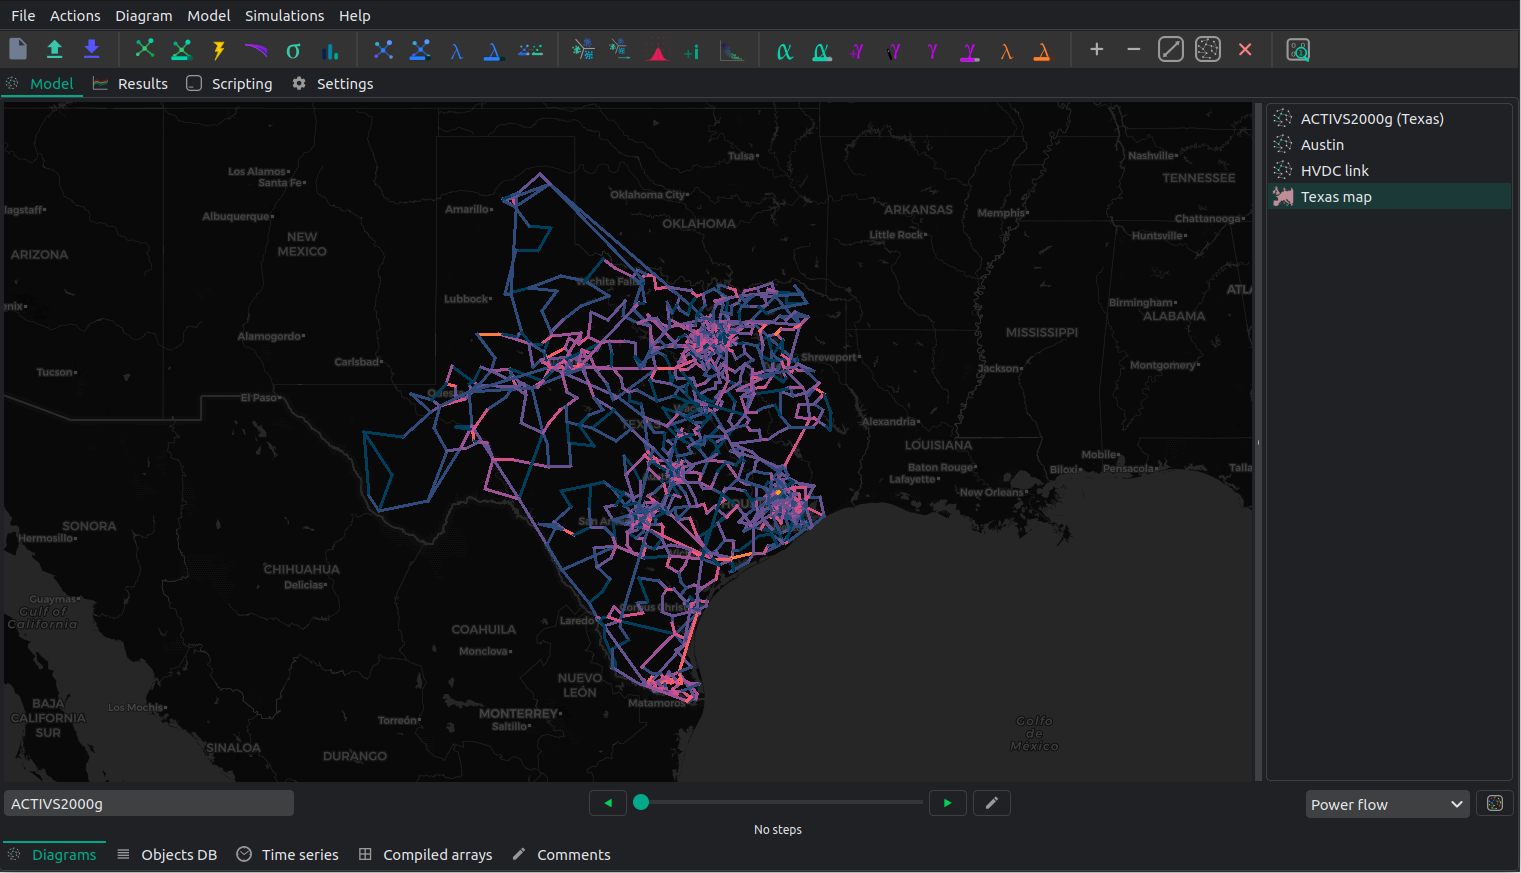
\includegraphics[width=0.8\linewidth]{figures/VeraGrid_main_page.png}
  \caption{VeraGrid main page. \textit{Source: VeraGrid documentation \cite{veragrid}.}}
  \label{fig:VeraGrid_main}
\end{figure}


\subsection{Previous requirements}

Before starting this thesis, it is necessary to have a solid understanding of power system dynamics, numerical methods for differential equations,
and programming in Python. Moreover, this section outlines specific theoretical background on the dynamic simulation of power systems, symbolic formulation and
differential-algebraic equations (DAEs). 

\subsubsection{Dynamic framework in Veragrid}

dfdg

\subsubsection{Symbolic formulation}

ewstrw

\subsubsection{Differential-Algebraic Equations (DAEs)}

CHECK!!

In many dynamic systems, including power systems, one encounters not only purely differential equations but also algebraic constraints linking the state
variables. Such systems are naturally represented by differential-algebraic equations (DAEs). Formally, a DAE is an equation of the form: 

\begin{equation}
  F\bigl(\dot{x}(t),\, x(t),\, y(t),\, t\bigr) = 0
\end{equation}


where $x(t)\in \mathbb{R}^n$ are the differential (dynamic) variables, $y(t)\in \mathbb{R}^m$ are algebraic variables, and the function
 $F$ encodes both the differential and algebraic relations. 
In contrast to an ordinary differential equation (ODE), not all derivatives \(\dot x\) can be explicitly solved from the system because some variables appear only 
algebraically(without derivative) \cite{PolitoDAE}.  

One common formulation is the so-called semi-explicit DAE of index 1:  
\begin{equation}
\begin{cases}
\dot x = f\bigl(x,\,y,\,t\bigr) \\
0 = g\bigl(x,\,y,\,t\bigr)
\end{cases}
\end{equation} 

where $f\colon \mathbb{R}^{n+m+1} \to \mathbb{R}^n$ and $g\colon \mathbb{R}^{n+m+1} \to \mathbb{R}^m$. In this form, one treats some variables $x$ as dynamic and others $y$
as constrained by algebraic equations. The condition for index 1 is that the partial Jacobian $\partial g / \partial y$ is nonsingular so that $y$ can be locally solved as
a function of $x$ and $t$ \cite{PolitoDAE}.  

An alternative is the fully implicit form:  

\begin{equation}
f\bigl(\dot x,\, x,\, y,\, t \bigr) = 0
\end{equation}

with no explicit separation of differential and algebraic parts. In that representation, one works directly with the combined vector $(\dot x, x, y)$ and the solver must treat 
the singularity in $\partial f / \partial \dot x$. Implicit DAEs are more general and often arise in multiphysics problems and constrained mechanical systems \cite{PolitoDAE}.  

\paragraph{Modeling power systems via DAEs}  
In power system dynamics, the network and algebraic constraints ( Kirchhoff’s current law, network admittance equations, etc.) naturally provide algebraic equations, 
while generator rotor dynamics, excitation systems, governor control, and other dynamic devices supply the differential equations. Thus a typical formulation is  

\begin{equation}
\begin{cases}
\dot x = f(x,\, y) \\
0 = g(x,\, y)
\end{cases}
\end{equation}

where $x$ includes rotor angles, speed deviations, internal voltages, control states, and $y$ includes bus voltages, phase angles, algebraic currents, and so on \cite{SauerPaiBook}. 
The coupling is strong: every time step, the algebraic network equations must be solved together with the differential updates, typically via Newton-Raphson or other Newton-based 
solvers applied to the full system Jacobian. In small-signal stability analysis, linearisation around an operating point yields the standard eigenvalue problem on the augmented 
state matrix, which preserves the structure of differential and algebraic coupling.  

This DAE-based representation ensures that the physical constraints of the network are never violated, and that stability and modal analysis reflect the full coupled system behavior,
rather than an oversimplified reduced ODE form.  


\newpage
\newpage

\section{Small-signal stability analysis}\label{Chap2}
%RMS SMALL SIGNAL STABILITY

\subsection{Power system stability}

Power system stability is defined as that property of a power system that enables it to 
remain in a state of operating equilibrium under normal conditions and to regain an acceptable 
state of equilibrium after being subjected to a disturbance \cite{StabilityAndControlKundur}. Other definitions
state not only the state of equilibrium must be acceptable but also most system variables must be 
bounded so that practically the entire system remains intact\cite{kundurDef}.


Although the primary concern is the behavior of the interconnected system as a whole, the stability of individual
components such as generators, motor loads, or regional subsystems; can be equally significant, particularly when 
localized instability does not propagate to the broader network. The system's dynamic behavior is governed by nonlinear 
interactions among its elements, and its response to perturbations is influenced by both the prevailing operating conditions
and the specific nature of the disturbance. Stability is understood around an equilibrium point and is subject to change
under small or large disturbances.

Power system stability is commonly classified depending on the pysical nature of the instability, the size of the disturbance 
considered and the devices, processes and time span that must be considered to assess stability \cite{kundurDef}.
The combination of these factors influence the methodologies, tools and considerations used in the analysis. The main categories of power system stability are 
described in the following enumeration.

\begin{itemize}
    \item \textit{Rotor angle stability}: The ability the ability of the interconnected synchronous machines in a power system 
    to remain in synchronism under normal operating conditions and to regain synchronism after being subjected to a
     small or large disturbance \cite{StabilityAndControlKundur}. A synchronous machine stays in synchronism when the 
     electromagnetic torque exactly balances the mechanical torque from the prime mover, producing zero net accelerating torque. 
     Stability therefore depends on the machine and its controls restoring that torque balance after a disturbance; failure to do 
     so causes rotor acceleration or deceleration and loss of synchronism.
    \item \textit{Voltage stability}: The capacity of the network to maintain acceptable voltage magnitudes at all buses 
    during normal operation and following disturbances, such that voltages do not decrease sustainedly. Loss of this 
    capacity manifests as progressive voltage drops and, ultimately, voltage collapse, which may force extensive load disconnection 
    or generalised service interruption.
    \item \textit{Frequency stability}: The capability of the system to preserve a near-nominal frequency following a major 
    imbalance between generation and demand, through inertial response and secondary/tertiary control actions. Inadequate frequency 
    stability results in sustained under-frequency or over-frequency transients that can damage equipment, trigger protective disconnections, 
    and precipitate broader system failure.
\end{itemize}

Due to the incrising penetration of power electronics into the grid, two new categories of stability have been considered \cite{DefStabExtended}.

  
\begin{itemize}
    \item \textit{Converter-driven stability}: Refers to oscillatory behaviour caused by control interactions in converter-interfaced generation (CIG). 
    Fast-interaction instabilities arise from high-frequency dynamics (hundreds of Hz to kHz) involving inner control loops and grid components. 
    Slow-interaction instabilities occur at low frequencies (<10 Hz), driven by PLL and outer-loop controls, especially 
    in weak grids. Synchronization issues and power transfer limits further compromise stability. 
    These phenomena differ from classical generator dynamics and require tailored mitigation strategies
    \item \textit{Ressonance stability}: Refers to the system's ability to withstand oscillatory 
    energy exchange without magnifying voltage, current, or torque beyond safe limits. It includes subsynchronous 
    resonance (SSR), which arises from interactions between series compensation and either mechanical shaft modes or 
    electrical generator characteristics. The mechanical form leads to torsional resonance, while the electrical 
    form—9 (Induction Generator Effect (IGE)) can cause self-excitation. Converter controls in DFIGs can exacerbate these 
    effects, leading to subsynchronous control interaction (SSCI). These phenomena pose risks to both mechanical integrity 
    and electrical equipment.
\end{itemize}


Rotor angle stability is inherent of classical power systems with synchronous machines. Modern power grids, with the increasing penetration of 
power electronics, have introduced new dynamics and interactions that can affect rotor angle stability. Converters decrease the inertia of the system
and have an effect on the electromechanical modes. However, the fundamental principles of rotor angle stability remain intact and still takes
a crucial role on stability analysis of power systems.

Therefore, understanding and analyzing rotor-angle stability remains essential for ensuring the overall reliability of power systems. 
Insufficient or negative synchronizing torque produces aperiodic, non-oscillatory transient instability that drives large rotor-angle deviations
and is typically studied with time-domain numerical integration. In contrast, the absence of adequate damping torque gives rise to small-disturbance
oscillatory instability.

In the context of this thesis, the focus is on rotor angle stability, particularly small-signal stability, its eigenvaule-based characterization, 
modal properties, and analysis methods. The following sections describe the theoretical background and methodologies used for small-signal stability 
analysis in power systems. 

\subsection{Stability of a dynamic system}

A dynamic system is considered stable if, when subjected to a disturbance, it returns to its original state or to a new equilibrium state without
exhibiting unbounded behavior. The equilibrium points are those states where all the derivatives $\dot{x}$ are zero, meaning the system is at rest
or in a steady state. 

Linearity affects on the stability of a system. The stability of a liner system is independent of the input and the initial conditions.
However, for a non-linear system, stability depends on the magnitude of the input and initial conditions. Depending on the region of the state-space,
stability is classified into the following categories:

\begin{itemize}
  \item \textit{Local stability}: the system is locally stable around an equilibrium point if when a small perturbation is applied,
  it remains around the equilibrium point. If as time increases it returns to the equilibrium point, it is locally asymptotically stable\cite{StabilityAndControlKundur}.
  \item \textit{Finite stability}: the system is finitely stable if when a perturbation of finite size is applied, it remains bounded and does not diverge to infinity.
  \item \textit{Global stability}: the system is globally stable if it returns to an equilibrium point for any initial condition in the whole state-space.
\end{itemize}

Therefore, linearizing a non-linear system around an equilibrium point allows to study its local stability as if it was a linear system. 

\subsection{Small-Signal stability}

Small-signal stability refers to the ability of a power system to maintain synchronism when subjected to 
small disturbances \cite{StabilityAndControlKundur}, such as minor load changes or small faults. These small disturbances
(typically within 1\%)occur frequently in power systems and allow the linearization of non-linear system equations
 around a specific operating point in order to perform analysis. The resulting linear representation enables the use
  of standard control engineering tools to assess system stability and dynamic performance \cite{SmallSignalCheah}.

The resulting instability due to those small perturbations can have two forms: Non-oscillatory unstability defined as an 
increase in rotor angle due to insufficient synchronizing torque and oscillatory unstability, oscillations of 
increasing magnitude due to insufficient damping torque \cite{StabilityAndControlKundur}. In practice, most of the 
instabilities come from insufficient damping torque. The following list summarizes the main oscillatory modes to consider:

\begin{itemize}
    \item \textit{Local modes}: Oscillations involving individual generators or small groups of units swinging 
    against the rest of the system, typically localized near a generating station.
    \item \textit{Inter area modes}: Low-frequency oscillations between large groups of generators in different 
    regions, often linked by weak transmission corridors.
    \item \textit{Control modes}: Oscillations arising from interactions between poorly tuned control systems—such 
    as exciters, speed governors, HVDC converters, or static var compensators.
    \item \textit{Torsional modes}: Oscillations associated with the mechanical shaft system of turbine-generators,
    which may become unstable due to interactions with control systems or series-compensated transmission lines.
\end{itemize}


Although small-signal analysis only applies to small variations around a fixed operating point, 
it remains a practical and widely used method for studying power system dynamics. By linearizing the system,
it allows to apply control theory tools like eigenvalue analysis and state-space modeling. 
This helps identify poorly damped modes and assess how the system responds to small disturbances. Despite its limitations,
it is a reliable approach for early detection of potential instabilities and for designing stabilizing controls.



\subsection{State-space representation}

Small-signal stability assessment methods are generally categorized into two main groups: state-space techniques
and frequency-domain techniques. State-space techniques allow one to represent the system using a set of first order
differential equations written in the following form:

\begin{equation}
    \dot{x} = f(x,u,t)
\end{equation}

Where $x$ is the state column vector that stores the state variables, $u$ is the input column vector that stores external
signals that influence the system performance and $t$ is time. The system can also not depend on time, that system is called 
time-invariant. It is also important to notw that state variables are the minimum amount of variables needed to represent the
system and be able to compute its future behaviour.

Often the purpose of the state-space representation is to look at a set of the system variables, called outputs $y$. Then, a new 
expression is added to the state-space representation:
\begin{equation}
    y = g(x,u,t)
\end{equation}

Where $y$ is the output column vector that stores the output variables.

A dynamic system can be described in many different ways depending on which variables are chosen as states, inputs, 
and outputs. These choices shape how the system behaves mathematically and how easily can it be analyzed. For example, 
using electrical quantities like voltage and current might be more practical for converter models, while mechanical variables 
such as rotor angle and speed are better suited for synchronous machines. The flexibility in selecting these variables allows
to adapt the model to the specific goals of the study while still ensuring that the essencial dynamics of the system are captured. 

State-space models are commonly represented in their matrix formulation as follows:

\begin{equation}
\dot{x} = Ax + Bu
\end{equation}
\begin{equation}
y = Cx + Du
\end{equation}

Where:

\begin{itemize}
  \item $x$ : state variables vector
  \item $u$ : system inputs vector
  \item $y$ : outputs vector
  \item $A$ : state matrix
  \item $B$ : input matrix
  \item $C$ : output matrix
  \item $D$ : direct transmission matrix
\end{itemize}

\subsubsection{Linearization of state-space models}

In order to linearize a non-linear state-space model, a small perturbation is applied around the operationg point (equilibrium point).

\begin{equation}
   \mathcal{X} \overset{\triangle}{=} x-x^*
\end{equation}
\begin{equation}
   \mathcal{Y} \overset{\triangle}{=} y-y^*
\end{equation}
\begin{equation}
   \mathcal{U} \overset{\triangle}{=} u-u^*
\end{equation}

Where $x^*$, $y^*$ and $u^*$ are the state, output and input vectors at the equilibrium point respectively. The new linearized state-space model is given by:

\vspace{2cm}

\begin{equation}
 \dot{\mathcal{X}} = A \mathcal{X} + B \mathcal{U}
\end{equation}
\begin{equation}
\mathcal{Y} = C \mathcal{X} + D \mathcal{U}
\end{equation}

Where the new matrices are computed as the Jacobian matrices of the non linear system evaluated at the equilibrium point:

\begin{center}
\begin{minipage}{0.45\textwidth}
\begin{equation}
  A =
\begin{bmatrix}
\frac{\partial f_{1}}{\partial x_{1}} & \cdots & \frac{\partial f_{1}}{\partial x_{n}} \\
\vdots & \ddots & \vdots \\
\frac{\partial f_{n}}{\partial x_{1}} & \cdots & \frac{\partial f_{n}}{\partial x_{n}}
\end{bmatrix}
\end{equation}
\end{minipage}\hfill
\begin{minipage}{0.45\textwidth}
\begin{equation}
  B =
\begin{bmatrix}
\frac{\partial f_{1}}{\partial u_{1}} & \cdots & \frac{\partial f_{1}}{\partial u_{n}} \\
\vdots & \ddots & \vdots \\
\frac{\partial f_{n}}{\partial u_{1}} & \cdots & \frac{\partial f_{n}}{\partial u_{n}}
\end{bmatrix}
\end{equation}
\end{minipage}

\vspace{1em}

\begin{minipage}{0.45\textwidth}
\begin{equation}
  C =
\begin{bmatrix}
\frac{\partial g_{1}}{\partial x_{1}} & \cdots & \frac{\partial g_{1}}{\partial x_{n}} \\
\vdots & \ddots & \vdots \\
\frac{\partial g_{n}}{\partial x_{1}} & \cdots & \frac{\partial g_{n}}{\partial x_{n}}
\end{bmatrix}
\end{equation}
\end{minipage}\hfill
\begin{minipage}{0.45\textwidth}
\begin{equation}
  D =
\begin{bmatrix}
\frac{\partial g_{1}}{\partial u_{1}} & \cdots & \frac{\partial g_{1}}{\partial u_{n}} \\
\vdots & \ddots & \vdots \\
\frac{\partial g_{n}}{\partial u_{1}} & \cdots & \frac{\partial g_{n}}{\partial u_{n}}
\end{bmatrix}
\end{equation}
\end{minipage}
\end{center}

For simplicity, the perturbation notation is often omitted, and the linearized state-space model is expressed as:
  
\begin{equation}
\Delta \dot{x} = A \Delta x + B \Delta u
\end{equation}
\begin{equation}
\Delta y = C \Delta x + D \Delta u
\end{equation}


\subsubsection{DAE to state-space representation}

In power systems, the dynamic behaviour is mathematically represented by a set of Differential-Algebraic Equations (DAEs) 
that capture the interaction between dynamic components and network constraints. This formulation naturally arises because power systems
 combine elements with both dynamic and instantaneous responses.

\begin{itemize}
\item \textit{Differential equations}: describe the time-dependent evolution of state variables associated with components that possess energy storage
 or control dynamics. These include synchronous generators (rotor angle and speed dynamics), excitation systems, governors, power electronic converters,
  and various control loops such as voltage and frequency regulators.
\item \textit{Algebraic equations}: represent the instantaneous electrical relationships and constraints imposed by the network. They stem primarily from Kirchhoff's laws,
 ensuring power balance and voltage-current consistency at each bus, as well as from static components like loads, transmission lines, and transformers, which are assumed
  to reach steady-state conditions instantaneously.
\end{itemize}


The explicit formulation of the DAE system is given by:
\begin{equation}
    T \dot{x} = f(x, y)
\end{equation}
\begin{equation}
    0 = g(x, y)
\end{equation}

Which is linearized around an equilibrium point as follows:

\begin{equation}
    T \Delta \dot{x} =\frac{\delta f}{\delta x}\Delta x + \frac{\delta f}{\delta y}\Delta y\\
\end{equation}
\begin{equation}
    0 =\frac{\delta g}{\delta x}\Delta x + \frac{\delta g}{\delta y}\Delta y\\
\end{equation}

From the second equation, $\Delta y$ can be expressed in terms of $\Delta x$:

\begin{equation}
    g_y\Delta y = -g_x \Delta x  \to \Delta y = - g_y^{-1} g_x \Delta x 
\end{equation}

And then substituted into the first equation:

\begin{equation}
    T \Delta \dot{x} = f_x\Delta x +f_y (- g_y^{-1} g_x  \Delta x) 
\end{equation}


Rearranging the equation gives the linearized state-space representation and the expression for the state matrix $A$:

\begin{equation}
    \Delta \dot{x} = T^{-1}(f_x-f_yg_y^{-1}g_x) \Delta x  \to A=T^{-1} (f_x-f_yg_y^{-1}g_x) 
\end{equation}


The A matrix encapsulates the dynamic interactions between the system's state variables, accounting for both the intrinsic dynamics of the components and the constraints imposed by the network. 
From the state matrix the stability assessment can be performed as explained in the next section.

\subsection{Stability assessment: Liapunov's first method}

The stability of a system can be studied in large-signal and small-signal therms. Stability \textit{in the large} needs to study the whole non-linear system. This method is complex and requires a high
computational effort. On the other hand, stability \textit{in the small} studies the system behaviour around an equilibrium point. This method is simpler and less computationally intensive, but it only 
provides information about the local stability of the system. Computing the eigenvalues of the state matrix $A$ allows to determine the small-signal stability of the system.

Eigenvalue analysis and participation factors (PF) are key tools for identifying dominant modes and evaluating system stability. These methods are well established in conventional 
power systems and are increasingly being applied to power-electronics-based systems, where dynamic behavior is often more complex and sensitive to operating conditions.

The eigenvalues $\lambda$ of the state matrix A, commonly referred to as the system's modes, characterize its small-signal stability according to the following criteria:

\begin{itemize}
  \item All modes satisfy $Re(\lambda) < 0$: the system is asymptotically stable
  \item All modes satisfy $Re(\lambda) \leq 0$ : the system is marginally stable
  \item At least one mode satisfies $Re(\lambda) > 0$: the system is unstable
\end{itemize}

When a linearized system has complex conjugate modes, they represent oscillatory modes in the dynamic response:

\begin{itemize}
  \item The real part determines damping:
  \begin{itemize}
    \item $Re(\lambda) < 0$: exponential decay
    \item $Re(\lambda) = 0$: oscillations persist indefinitely
    \item $Re(\lambda) > 0$: exponential growth
  \end{itemize}
  \item The imaginary part determines the oscillation frequency defined as: $f = \frac{Im(\lambda)}{2\pi}$
\end{itemize}

An other way to look at the damping of a mode is through the damping ratio $\zeta$. The damping ratio is a dimensionless measure that describes how oscillations 
in a system decay after a disturbance. It is defined as the ratio of actual damping to critical damping. The critical damping is the minimum amount of damping that prevents oscillations. 
The damping ratio is given by: 

\begin{equation}
  \zeta = -  \frac{Re(\lambda)}{\sqrt{Re(\lambda)^2+Im(\lambda)^2}}
\end{equation}

Where $Re(\lambda)$ is the real part of the eigenvalue and $Im(\lambda)$ is the imaginary part of the eigenvalue. The interpretation of the damping ratio is described below.

\begin{itemize}
  \item $\zeta < 0$: \textit{Unstable oscillations.} The system exhibits modes that grow exponentially with time, caused by eigenvalues located in the right half of the complex plane.
  \item $\zeta = 0$: \textit{Marginal stability.} The system produces undamped, sustained oscillations since the eigenvalues lie exactly on the imaginary axis.
  \item $0 < \zeta < 1$: \textit{Stable oscillatory response.} The system returns to its equilibrium point through oscillations that gradually decay over time. In practical terms, a damping ratio of about $\zeta = 0.05$ is generally considered sufficient for well-damped behaviour.
  \item $\zeta = 1$: \textit{Critical damping.} The system returns to equilibrium without oscillations, reaching the steady state in the shortest possible time without overshoot.
\end{itemize}

Finally, participation factors quantify the relative influence of each state variable on the different dynamic modes of the system. In essence,
they indicate how much a given state contributes to a specific mode and, conversely, how strongly that mode affects the state.
This dual interpretation makes participation factors a valuable tool for understanding the internal structure of system dynamics.

In the context of power systems, participation factors play a key role in identifying the physical origin of oscillations and instabilities.
By analysing these factors, it is possible to determine which components—such as generators, controllers, or converter units—are most involved in poorly damped or unstable modes.
This information supports targeted actions for control tuning, model validation, and stability improvement. Participation factors are calculated as follows:

\begin{equation}
PF_{i,k} = W_{i,k} \cdot V_{i,k}
\end{equation}

Where:
\begin{itemize}
  \item $PF_{i,k}$ is the participation factor of the $k$-th state variable to the $i$-th mode.
  \item $W_{i,k}$ is the left eigenvector of the $k$-th state variable to the $i$-th mode of matrix $A$. It satisifies $w^T A = \lambda w^T$.
  \item $V_{i,k}$ is the right eigenvector of the $k$-th state variable to the $i$-th mode of matrix $A$. It satisifies $A v= \lambda v$.
\end{itemize}

The graphical representation of the eigenvalues in the complex plane, provides a visual tool for assessing system stability. Then, it is possible to identify
the stability of the system and the oscillation of the modes at a glance. An example of an eigenvalue plot is shown in Figure \ref{fig:eigenvalue_plot}.

\begin{figure}[H]
  \centering
  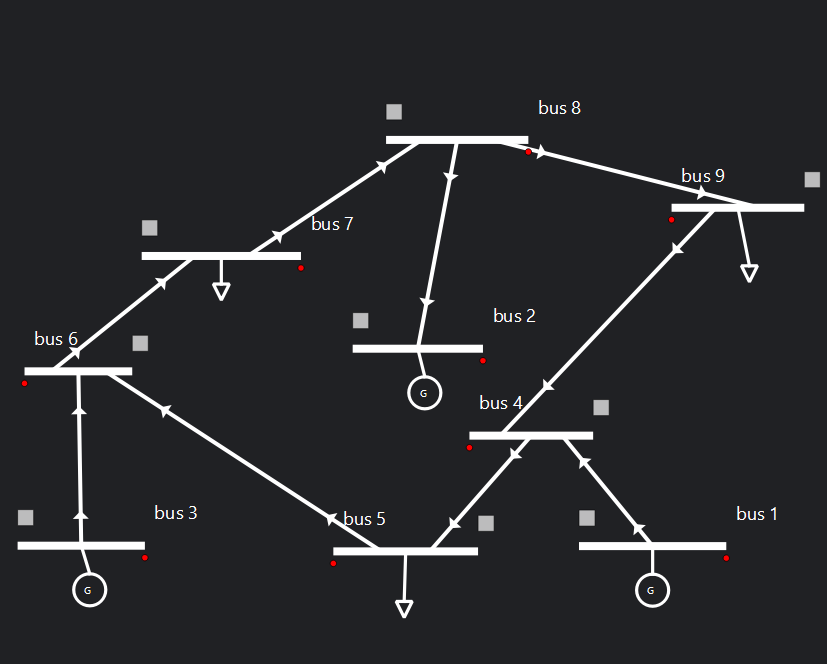
\includegraphics[width= 250 px]{Images/case9_topo.png}
  \caption{Schematic of the 9-bus grid.}
  \label{fig:eigenvalues_plot_example}
\end{figure}



\newpage

\section{Grid Model}\label{Chap3}
%%%POWER FLOW EQUATIONS

Once all the elements of the grid have been defined, the model of the power flow can be properly explained.
The approach chosen is aligned with the models proposed by GridCal, which make use of the Universal Branch Model to describe 
the admittance matrices of the branches. The power flow model used during this project has been the Bus Injection Model (BIM),
which will be calculated at each bus of the grid, and has to be equal to zero for the system to be in equilibrium. This model
relates voltages, power transfer, tap variables, generation and demand, which are the variables of the optimization problem.

The notation used throughout this work is as follows: vectors are denoted in bold (can be both upper or lowercase), matrices are denoted in uppercase, and scalars are denoted in lowercase.
Vectors that are transformed in diagonal matrices appear within square brackets. Vectors that slice other vectors using their values as indexes appear after the slice vector within curly brackets.

\subsection{Power Flow Equations}

The full construction of the power flow equations is shown, since some intermediate steps can be useful for later purposes. 
The first important equation is the power transfer that occurs between two nodes connected with branch, modelled using the Flexible Universal Branch Model for the $k$ branch as in Equations~\eqref{eq:Y_prim1} and~\eqref{eq:Y_prim2}.
They contain the information of a single line. In the grid model used, $y_{ff}$, $y_{ft}$, $y_{tf}$ and $y_{tt}$ are vectors of length $l$ that store 
these primitives of the admittance matrix for all the branches in the model.

Consider the connectivity matrices $C_f$ and $C_t$, with size $k$ x $l$ that relate the index of the 'from' and 'to' buses to the index of their branch as follows:

\begin{equation}
    C_{f_{ki}} =    
    \begin{cases}
    1, & \text{for } k == (i, j) \quad \forall j \in \bm {N}\\
    0, & \text{otherwise}
    \end{cases}
\end{equation}

\begin{equation}
    C_{t_{kj}} =    
    \begin{cases}
    1, & \text{for } k == (i, j) \quad \forall i \in \bm {N}\\
    0, & \text{otherwise}
    \end{cases}
\end{equation}

Using these connectivity matrices and the primitives, $from$ and $to$ admittance matrices can be constructed. The $to$ admittance matrix contains the elements of the 
admittance matrix that are connected to the 'to' bus of the branch, while the $from$ admittance matrix contains the elements connected to the 'from' bus of the branch. 
The bus admittance matrix $Y_{bus}$, which contains all the information needed to calculate the power flow, can then be constructed.

\begin{equation}
    \begin{split}
    Y_f &= [\bm{Y_{ff}}]\, C_f + [\bm{Y_{ft}}]\, C_t \\
    Y_t &= [\bm{Y_{tf}}]\, C_f + [\bm{Y_{tt}}]\, C_t \\
    Y_{bus} &= C_f^\top {Y_f} + C_t^\top \bm{Y_t} + [\bm{Y_{sh}}]
    \end{split}
\end{equation}

where the brackets indicate that the vector is transformed into a diagonal matrix and the $[\bm{Y_{sh}}]$ matrix contains the shunt admittance of each bus,
which is calculated for each bus by GridCal modeller. The resulting matrices have size \textit{m} x \textit{n}.

The model used to calculate the power balance of the system is the bus injection model, which is based on the equality between the power injected in a bus and
power flowing out of it. The injection can come from generators connected at the bus or lines from buses while 
the outflow goes to demand connected to the bus or lines that transport energy to other buses.

The vector of complex power injections from lines $\bm{S_{bus}}$ is given by the following equations:

\begin{equation}
    \bm{S_{bus}} = [\bm{V}] (Y_{bus} \bm{V})^*
    \label{Eq:Sbus}
\end{equation}

where $\bm{V}$ is the vector of the complex voltages of the buses calculated as:

\begin{equation}
    \bm{\mathcal{V}} e^{j\bm{\theta}} 
\end{equation}

using element to element multiplication, and being $\mathcal{V}$ the vector of voltage modules and $\theta$ the vector of voltage angles. The complete balance can be now calculated as:

\begin{equation}
    \bm{G^{S}_{bus}} = \bm{S_{bus}} - \bm{S_{bus}^{g}} + \bm{S_{bus}^{d}}  = \bm{0} \quad \text{(equilibrium)}
    \label{eq:GSbus} 
\end{equation}

where $\bm{S_{bus}^{g}}$ is the power generated at the buses, and  $\bm{S_{bus}^{d}}$ the power consumed at the buses. The notation $\bm{G^{S}}$ will be useful later to refer to this balance as an equality constraint of the optimization problem.

One particularity to be considered is that there could be multiple generators or loads connected to the same bus. For the present work, there is no segregation of loads and the bus demand is obtained directly from GridCal, but it could be consider
to model load flexibility and shedding. For generations, the separation has to be done as there could be differences in price or operational limits. To do so, $\bm{S^{g}}$ is obtained through the use of the \textit{n} x \textit{ng} connectivity matrix $C_{G}$:

\begin{equation}
    \bm{S_{bus}^{g}} = C_{G} \bm{S^{g}}
    \label{Eq:Gen}
\end{equation}

For buses that are part of a DC link, the power balance has to account for the power transferred through the link.

\newcommand{\pluseq}{\mathrel{{+}{=}}}
\newcommand{\minuseq}{\mathrel{{-}{=}}}

\begin{equation}
    \begin{split}
        \bm{G_{bus}^{S}} \{\bm{fdc}\} \pluseq  \bm{P_{dc}}\{\bm{dc}\} \\
        \bm{G_{bus}^{S}} \{\bm{tdc}\} \minuseq \bm{P_{dc}}\{\bm{dc}\}
    \end{split}
\end{equation}


In addition to the bus power balance, the line power balance has to be considered to ensure that operational limits of the lines are not exceeded. The power
flowing through a line can be calculated using the $from$ and $to$ admittance matrices and the voltages of the buses connected to the line. Both sides of the
lines have to be considered, since the powers at the ends are not equal and the direction of the flow can change depending on grid conditions.

\begin{equation}
    \begin{split}
    \bm{V_f} &= C_f \bm{V} \\
    \bm{V_t} &= C_t \bm{V} \\
    \bm{S_f} &= [\bm{V_f}] (Y_f \bm{V})^*\\
    \bm{S_t} &= [\bm{V_t}] (Y_t \bm{V})^*
    \end{split}
\end{equation}

Here it is important to note that the vector $\bm{V_f}$ will contain the voltage value of the $from$ bus of each line, which means there can be some buses appearing more than one time.

\subsection{Operational limits}

Each element of the grid has its owns operational limits that have to be respected. The limits are stored in lists of length equal to the respective element count.
These limits correspond to inequalities of the optimization problem. The notation $\bm{H^{I}}$ is used to identify to each different limit.

\subsubsection{Nodal voltage limits}

The voltage module limits of the buses are stored in the $\bm{V_{max}}$ and $\bm{V_{min}}$ arrays, with its value in per unit. The limits are checked using the following equations:

\begin{equation}
    \begin{split}
    \bm{H^{v_{u}}} &= \bm{\mathcal{V}} - \bm{V_{max}} \leq \bm{0} \quad \text{(upper limit)}\\
    \bm{H^{v_{l}}} &= \bm{V_{min}} - \bm{\mathcal{V}} \leq \bm{0} \quad \text{(lower limit)}
    \end{split}
\end{equation}

\subsubsection{Generation limits}

The generation limits apply to both the active and reactive power of the generators. They are stored in the $P_{max}$, $P_{min}$, $Q_{max}$ and $Q_{min}$ lists,
with its value in per unit. The limits are checked using the following equations:

\begin{equation}
    \begin{split}
    \bm{H^{P_{u}}} &= \bm{P_g} - \bm{P_{max}} \leq \bm{0} \quad \text{(upper limit)}\\
    \bm{H^{P_{l}}} &= \bm{P_{min}} - \bm{P_g} \leq \bm{0} \quad \text{(lower limit)}\\
    \bm{H^{Q_{u}}} &= \bm{Q_g} - \bm{Q_{max}} \leq \bm{0} \quad \text{(upper limit)}\\
    \bm{H^{Q_{l}}} &= \bm{Q_{min}} - \bm{Q_g} \leq \bm{0} \quad \text{(lower limit)}
    \end{split}
\end{equation}

An additional constraint over the generation is the reactive power limitations due to the generator capability curves. These curves can be modelled by piecewise defined function, 
but in the formulation of the problem they have been considered much simpler, and by default they are not applied. The following constraint models the reactive power limits of the generators:

\begin{equation}
    \begin{split}
    \bm{H^{ctQ}} &= \bm{Q_g}^2 - \bm{tanmax}^2 \bm{P_{g}}^2 \leq \bm{0}\\
    \end{split}
\end{equation}

where $\bm{tanmax}$ is the maximum value of the tangent of the angle between the active and reactive power of the generator.

\subsubsection{Transformer limits}

The controllable transformers will have their limits for the controllable variables limited. The limits are similar to the previous:

\begin{equation}
    \begin{split}
    \bm{H^{m_{p_{u}}}} &= \bm{m_{p}} - \bm{m_{p_{max}}} \leq \bm{0} \quad \text{(upper limit)}\\
    \bm{H^{m_{p_{l}}}} &= \bm{m_{p_{min}}} - \bm{m_{p}} \leq \bm{0} \quad \text{(lower limit)}\\
    \bm{H^{\tau_{u}}} &= \bm{\tau} - \bm{\tau_{max}} \leq \bm{0} \quad \text{(upper limit)}\\
    \bm{H^{\tau_{l}}} &= \bm{\tau_{min}} - \bm{\tau} \leq \bm{0} \quad \text{(lower limit)}
    \end{split}
\end{equation}

\subsubsection{Line limits}

The line limits will be checked only for the monitored branches, which is a subset of size $m$ from the total number of branches $l$, considering the rating of each line in per unit. Since the direction of the flow is not known, and to
avoid using absolute values, this constraint is considered quadratically.

\begin{equation}
    \begin{split}
    \bm{H^{S_f}} &= \bm{S_f} \bm{S_f}^* - \bm{S_{max}}^2 \leq \bm{0} \\
    \bm{H^{S_t}} &= \bm{S_t} \bm{S_t}^* - \bm{S_{max}}^2 \leq \bm{0} 
    \end{split}
\end{equation}

\subsubsection{Bound slack variables}

So far, all the constraints described has physical meaning and are related to the grid model. The last set of constraints are related to the optimization problem
and are used to improve, or even make possible, the convergence of the solver. The bound slacks are used to allow the solution to surpass some operational 
limits in order to find a feasible solution. Of course, it should come at a cost and the objective function will be used to penalize this behavior. 

These bound slacks are applied to the voltage limits and to the line limits, allowing slight over or undervoltages and some overloads.
The constraint equations are modified, and the slack variables are imposed to be positive. The equations are as follows:

\begin{equation}
    \begin{split}
    \bm{H^{v_{u}}} &= \bm{\mathcal{V}} - \bm{V_{max}} - \bm{sl_{v_{max}}} \leq \bm{0} \quad \text{(upper limit)}\\
    \bm{H^{v_{l}}} &= \bm{V_{min}} - \bm{\mathcal{V}} - \bm{sl_{v_{min}}} \leq \bm{0} \quad \text{(lower limit)}\\
    \bm{H^{S_f}} &= \bm{S_f} \bm{S_f}^* - \bm{S_{max}}^2 - \bm{sl_{sf}} \leq \bm{0} \quad \text{(from limit)}\\
    \bm{H^{S_t}} &= \bm{S_t} \bm{S_t}^* - \bm{S_{max}}^2 - \bm{sl_{st}} \leq \bm{0} \quad \text{(to limit)} \\
    - \bm{H^{sl_{v_{max}}}} &\leq \bm{0} \\
    - \bm{H^{sl_{v_{min}}}} &\leq \bm{0}\\
    - \bm{H^{sl_{sf}}} &\leq \bm{0}\\
    - \bm{H^{sl_{st}}} &\leq \bm{0}
\end{split}
\end{equation}

The use of this bound slacks is optional and can be removed from the optimization problem if the user prefers to have a solution in compliance with the 
established limits.








\newpage

\section{Optimization Problem}\label{Chap4}
%OPTIMIZATION PROBLEM

This section describes the optimization model used to solve the AC Optimal Power Flow problem. The mathematical formulation
of this problem is presented using abstract notation of the Karush-Kuhn-Tucker (KKT) conditions for optimization problems, which later on
will regain a more practical form. The implementation of the solver is also described, as well as the pseudo-code used to
solve the problem. The general theory of optimization can be found in the book of Boyd and Vandenberghe \cite{boyd2004convex}, with a more detailed explanation of the IPM in Chapter 19 of
Nocedal and Wright's book \cite{NocedalWright}, and the adaptation of this theory to a more compact formulation can be reviewed in the Matpower Interior
Point Solver documentation \cite{zimmerman2016mips} \cite{wang2007computational}.


\subsection{Optimization problem}

The general optimization problem involving equality and inequality constraints can be formulated as follows:

\begin{equation}
    \begin{split}
        \text{min} \quad & f(\bm{x}) \\
        \text{s.t.} \quad & \bm{G}(\bm{x}) = \bm{0} \\
         & \bm{H}(\bm{x}) \leq \bm{0}
    \end{split}
    \label{eq:opt_prob}
\end{equation}

where $\bm{x} \in \mathbb{R}^n$, being $n$ the number of decision variables, $f(x)$ is the function to be minimized which typically 
accounts for the generation cost, $\bm{G}(\bm{x})$ is the set of $n_e$ equality constraints of the problem, and $\bm{H}(\bm{x})$ is the set of $n_i$ inequalities. 

The problem will be solved using the barrier parameter method, which consists of solving the optimization problems sequencially with
different values of the barrier parameter $\gamma$. The barrier parameter is an IPM methodology used to penalize the violation of the inequality 
constraints in the problem, which are turned into equalities of the form $\bm{H(x)} + \bm{Z} = \bm{0}$ by the addition of the positive slack variables $\bm{Z}$.

The Lagrangian of the problem is defined by:

\begin{equation}
    \mathcal{L}(\bm{x}, \bm{Z}, \bm{\lambda}, \bm{\mu}) = f(\bm{x}) + \bm{\lambda}^\top \bm{G}(\bm{x}) + \bm{\mu}^\top (\bm{H}(\bm{x})+\bm{Z}) - \gamma \sum_{i=1}^{n_i} \log(z_i) 
    \label{eq:lag}
\end{equation}
    
where $\bm{\lambda}$ and $\bm{\mu}$ are the Lagrange multipliers associated with the equality and inequality constraints respectively, the superindex $\top$ is used to indicate the transposition
of a vector and the elements of the sum $z_i$ correspond to each value of the vector $\bm{Z}$.

The KKT conditions are a set of equations that must be satisfied by the solution of the optimization problem. These conditions are a result of 
imposing that the partial derivatives of the Lagrangian in the $(x, Z, \lambda, \mu)$ variable space equals 0, as shown in Equation~\eqref{eq:block1}.

\begin{equation}
    \begin{split}
    \nabla_{x, Z, \lambda, \mu} \mathcal{L}(\bm{x}, \bm{Z}, \bm{\lambda}, \bm{\mu}) &= \bm{0} \\
    \end{split}
    \end{equation}

\begin{equation}
    \begin{split}
    \bm{\mathcal{L}_x}(\bm{x}, \bm{Z}, \bm{\lambda}, \bm{\mu}) &=  f_x + \bm{\lambda}^\top G_x + \bm{\mu}^\top H_x = \bm{0} \\
    \bm{\mathcal{L}_Z}(\bm{x}, \bm{Z}, \bm{\lambda}, \bm{\mu}) &=  \bm{\mu}^\top - \gamma \bm{1}_{n_i}^\top[\bm{Z}]^{-1} = \bm{0} \\
    \bm{\mathcal{L}_{\lambda}}(\bm{x}, \bm{Z}, \bm{\lambda}, \bm{\mu}) &=  \bm{G}^\top(\bm{x}) = \bm{0} \\
    \bm{\mathcal{L}_{\mu}}(\bm{x}, \bm{Z}, \bm{\lambda}, \bm{\mu}) &=  \bm{H}^\top(\bm{x}) + \bm{Z}^\top = \bm{0} \\
    \end{split}
    \label{eq:block1}
\end{equation}

where $\bm{1}_{n_i}$ is a vector of ones of length $n_i$, and $\gamma$ is the barrier parameter that will be updated in each iteration of the solver until
reaching a value close to zero. The notation $f_{\bm{X}}$ indicates the gradient of the given function $f$ with respect to the vector $\bm{X}$.

The first gradient corresponds to the stationary condition of the problem, the second gradient corresponds to the complementary slackness,
and the other two gradients correspond to the primal feasibility conditions of the problem. These conditions, alongside the dual feasibility 
condition $Z_i, \mu_i \geq 0 \quad \forall i$, are necessary and sufficient for the solution of the optimization problem.
The resulting set of equations will be solved computationally due to the non-convex nature of the problem. For this type of general problem,
the approach chosen is the use of an Interior Point Method (IPM) solver.

% \begin{align}
%     %\label{eq:block1}
% \nabla f(\bm{x}) + \bm{A_e}^\top(\bm{x}) \bm{\lambda} + \bm{A_i}^\top(\bm{x}) \bm{\mu} &= \bm{0} \\
% [\bm{s}] \bm{z} - \mu \bm{1}_{n_i} &= \bm{0} \\
% \bm{G}(\bm{x}) &= \bm{0} \\
% \bm{H}(\bm{x}) + \bm{Z} &= \bm{0} \\
% \bm{s_i}, \bm{z_i} &\geq \bm{0} \quad \forall i
% \label{eq:block2}
% \end{align}

% where $\nabla f(\bm{x})$ is the gradient of the objective function and takes the form 
% $[\frac{\partial f}{\partial x_1}, \frac{\partial f}{\partial x_2}, ..., \frac{\partial f}{\partial x_n}]^\top$, $\bm{A_e} (\bm{x})$ is a matrix 
% concatenating the gradients of the equality constraints as $[\nabla g_1^\top, \nabla g_2^\top, ..., \nabla g_{n_e}^\top]$ with $n_e$ the number of equality constraints,
% $\bm{A_i} (\bm{x})$ is a matrix concatenating the gradients of the inequality constraints as $[\nabla h_1^\top, \nabla h_2^\top, ..., \nabla h_{n_i}^\top]$ with $n_i$ 
% the number of inequality constraints, $\bm{y}$ and $\bm{z}$ are column vectors of Lagrange multipliers of lengths $n_e$ and $n_i$ respectively, 
% $\bm{s}$ is a column vector of length $n_i$, and $\mu$ is the barrier parameter which will take different values for each iteration of the solving process.



\subsection{Interior Point Method solver}

The choice of this type of solver is regarded as the best option to deal with non-linear optimization, as shown in the dedicated chapter 19 in 
Nocedal and Wright's book. %%% ADD REFERENCE
The IPM solver is a type of optimization algorithm that solves the KKT conditions of the problem iteratively. There are multiple algorithms that can be used,
although the one presented in this project is the Newton-Raphson. Since this algorithm will be used by the Spanish TSO for country-sized grids, the scalability of the solver 
is a key factor to consider.  In reference \cite{abaali2018comparison}, this algorithm is compared with the Gauss-Seidel algorithm, yielding better scalability 
for the Newton-Raphson method. 

Some optimization solver packages such as IPOPT were considered, but creating a tailored solver and integrating it in GridCal was considered the best option, as it 
avoids depending on third-party software, while also allowing the customization of its behavior.

There can be improvements to this method as presented in the literature, %%ADD REFERENCES%%%%%%%%%%%%%%%%%%%%%%%%%%%%%%%%%%%%%%%%%
but for the purpose of this project, the IPM has been implemented directly using the Newton-Raphson method with a step-control mechanism. 

The Newton-Raphson iterative process that will find the roots of the KKT conditions can be described as in Algorithm 1.

\begin{algorithm}
\caption{Newton-Raphson Iterative Process}
\begin{algorithmic}[1]
\STATE Initialize $\bm{x}_0$, tolerance $\epsilon$, and set $k = 0$
\WHILE{$||\bm{f}(\bm{x}_k)|| > \epsilon$}
    \STATE Compute the Jacobian matrix $J(\bm{x}_k)$
    \STATE Solve $J(\bm{x}_k) \Delta \bm{x}_k = -\bm{f}(\bm{x}_k)$ for $\Delta \bm{x}_k$
    \STATE Apply step control to $\Delta \bm{x}_k$
    \STATE Update $\bm{x}_{k+1} = \bm{x}_k + \Delta \bm{x}_k$
    \STATE $k = k + 1$
\ENDWHILE
\end{algorithmic}
\end{algorithm}

The algorithm will perform several Newton-Raphson steps until the convergence criteria is met, meaning that equations~\eqref{eq:block1} are solved. 
The expanded formulation of the system solved at each step is:

\begin{equation}
    - \begin{pmatrix}
        \bm{\mathcal{L}_{xx}} & \bm{0} & \bm{G_x}^\top(\bm{x}) & \bm{H_x}^\top(\bm{x}) \\ 
        \bm{0} & [\bm{\mu}] & \bm{0} & [\bm{Z}] \\
        \bm{G_x}(\bm{x}) & \bm{0} & \bm{0} & \bm{0} \\
        \bm{H_x}(\bm{x}) & \bm{I} & \bm{0} & \bm{0}
    \end{pmatrix}
    \begin{pmatrix}
        \bm{\Delta x} \\
        \bm{\Delta Z} \\
        \bm{\Delta \lambda} \\
        \bm{\Delta \mu}
    \end{pmatrix} = 
    \begin{pmatrix}
        \mathcal{L}_x^\top \\
[\bm{\mu}] \bm{Z} - \gamma \bm{1}_{n_i} \\
\bm{G}(\bm{x}) \\
\bm{H}(\bm{x}) + \bm{Z}
    \end{pmatrix}
    \label{eq:Jacob_full}
\end{equation}

where $\bm{\Delta x}$ represents the variation of $\bm{x}$ (and similarly to $\bm{s}$, $\bm{y}$, $\bm{z}$), $\bm{I}$ is the identity matrix, and the term  
$\bm{\mathcal{L}_{xx}}$ is the derivative of the first KKT condition, which was already the gradient of the Lagrangian of the problem. This Hessian matrix
is the element that has the most computational cost to be calculated. Its calculation will have to be the most optimized possible to ensure the solver's scalability.

Note that dual feasibility condition $Z_i, \mu_i \geq 0 \quad \forall i$ is not included in the system of equations. This condition will be enforced by the algorithm when choosing
the step length of the iteration when updating the variables.

This system of equations can be further reduced using methods that can be found in \cite{NocedalWright}, derived with detail in \cite{zimmerman2016mips}. 
The relevant equations obtained during the reduction process are shown in Equations~\eqref{eq:red1} and~\eqref{eq:red2}.

\newcommand{\ones}{\mathbf{1}}

\begin{equation}
    \begin{cases}
        [\bm{\mu}] \Delta \bm{Z} + [\bm{Z}] \Delta \bm{\mu} &= -[\bm{\mu}] \bm{Z} + \gamma \ones_{n_i}  \\
        [\bm{Z}] \Delta \bm{\mu} &= -[\bm{Z}] \bm{\mu} + \gamma \ones_{n_i}  - [\bm{\mu}] \Delta \bm{Z} \\
        \Delta \bm{\mu} &= -\bm{\mu} + [\bm{Z}]^{-1} (\gamma \ones_{n_i}  - [\bm{\mu}] \Delta \bm{Z}).
    \end{cases}
    \label{eq:red1}
\end{equation}  

\begin{equation}
    \begin{cases}
        \bm{H}_x \Delta \bm{X} + \Delta \bm{Z} &= -\bm{H}(\bm{X}) - \bm{Z} \\
        \Delta \bm{Z} &= -\bm{H}(\bm{X}) - \bm{Z} - \bm{H}_x \Delta \bm{X}.
    \end{cases}
    \label{eq:red2}
\end{equation}

\begin{equation}
    \begin{cases}
    \bm{M} &\equiv \bm{\mathcal{L}_{xx}} + \bm{H_x}^\top [\bm{Z}]^{-1} [\bm{\mu}] \bm{H}_{\bm{x}} \\
    &= \bm{f_{xx}} + \bm{G_{xx}}(\bm{\lambda}) + \bm{H_{xx}}(\bm{\mu}) + \bm{H_{x}}^\top [\bm{Z}]^{-1} [\bm{\mu}] \bm{H_x}.
    \end{cases}
    \label{eq:red3}
\end{equation}

\begin{equation}
    \begin{cases}
    \bm{N} &\equiv \bm{\mathcal{L}_x}^\top + \bm{H_x}^\top [\bm{Z}]^{-1} (\gamma \bm{1_{n_i}} + [\bm{\mu}] \bm{H}(\bm{x})) \\
    &= \bm{f_x}^\top + \bm{G_x}^\top \bm{\lambda} + \bm{H_x}^\top \bm{\mu} + \bm{H_x}^\top [\bm{Z}]^{-1} (\gamma \bm{1_{n_i}} + [\bm{\mu}] \bm{H}(\bm{x})).
    \end{cases}
    \label{eq:red4}
\end{equation}

This transformation will make possible to reduce the size of Equation~\eqref{eq:Jacob_full} to a system of equations over $(\bm{x}, \bm{\lambda})$ instead, and then calculating the 
terms corresponding to the inequalities using the expressions shown in Equation~\eqref{eq:red1}. This smaller size reduces the computational time of computing such a large system. 
The resulting reduced system is the following:

\begin{equation}
    \begin{bmatrix}
    \bm{M} & \bm{G}_{\bm{x}}^\top \\
    \bm{G}_{\bm{x}} & \bm{0}
    \end{bmatrix}
    \begin{bmatrix}
    \Delta \bm{x} \\
    \Delta \bm{\lambda}
    \end{bmatrix}
    =
    \begin{bmatrix}
    -\bm{N} \\
    -\bm{G}(\bm{x})
    \end{bmatrix}
    \label{eq:red5}
\end{equation}

The solver will firstly solve this smaller matricial problem to obtain the variation of the decision variables and the Lagrange multipliers associated with the equality constraints, and then
it will compute the inequality terms using Equations~\eqref{eq:red1} and~\eqref{eq:red2}.

Before proceeding to update the values of the variables, there will be two additional steps to be taken. The first one is to ensure that 
the dual feasibility condition $$\bm{Z_i}, \bm{\mu_i} \geq 0 \quad \forall i$$ is met. This will be done by using the maximum step length such that 
the values of the multipliers remain positive. The calculation of this step length is shown at Equation~\eqref{eq:step_length}.

\begin{equation}
    \begin{split}
    \alpha_p &= \min \left( \tau \cdot \min \left(- \frac{\bm{Z}}{\Delta\bm{Z}}\right), 1 \right) \\
    \alpha_d &= \min \left( \tau \cdot \min \left(- \frac{\bm{\mu}}{\Delta\bm{\mu}}\right), 1 \right)
    \end{split}
    \label{eq:step_length}
\end{equation}

where $\tau$ is a parameter that will be set to a value really close to 1, without exceeding it (i.e. 0.9995). 

This step length will be tested to ensure that it is not too large as it could lead to divergence of the algorithm. This will be done by using a
step control mechanism that will reduce the step length if the conditions are not met. The step control mechanism will update just the decision variables $x$,
using the Lagrangian of the system as a reference. The step control mechanism is described in Algorithm 2.

\begin{algorithm}
    \caption{Step Control}
    \begin{algorithmic}[2]
    \STATE Initialize  $\mathcal{L}_0 = f(\bm{x}) + \bm{\lambda}^\top \bm{G(x)} + \bm{\mu}^\top \bm{H(x)} - \gamma \sum_{i=1}^{n_i} \log(Z_i)$, $\alpha = 1$, use
    its gradient $\bm{\mathcal{L}_x}$ and hessian $\bm{\mathcal{L}_{xx}}$ previously used for the Jacobian, and set $\alpha = trust$
    \WHILE{$i < step\_control\_iterations$}
        \STATE $\Delta \bm{x}_1 = \alpha \Delta \bm{x}$
        \STATE $\bm{x}_1 = \bm{x} + \Delta \bm{x}_1$
        \STATE Compute $\mathcal{L}_1$ and $\mathcal{L}_{x_1}$
        \STATE $\rho = \frac{\mathcal{L}_1 - \mathcal{L}}{\bm{\mathcal{L}_x} \Delta \bm{x_1} + 0.5 \Delta \bm{x_1}^\top \bm{\mathcal{L}_{xx}}\Delta \bm{x_1}}$ 
        \IF{$\rho \leq \rho_{lower}$ \textbf{or} $\rho \geq \rho_{upper}$}
            \STATE $i = i+1$
            \STATE $\alpha = \alpha / 2$
        \ENDIF 
    \ENDWHILE
    \end{algorithmic}
\end{algorithm}

This will reduce all the step sizes if the new Lagrangian does not accomplish the condition. If this condition is not activated, then $\alpha = 1$.
Now, the values of all the variables and multipliers can be updated with the final values of the step length: 

\begin{equation}
    \begin{split}
    \bm{x} &\leftarrow \bm{x} + \alpha\alpha_p \Delta \bm{x} \\
    \bm{Z} &\leftarrow \bm{Z} + \alpha\alpha_p \Delta \bm{Z} \\
    \bm{\lambda} &\leftarrow \bm{\lambda} + \alpha\alpha_d \Delta \bm{\lambda} \\
    \bm{\mu} &\leftarrow \bm{\mu} + \alpha\alpha_d \Delta \bm{\mu}
    \end{split}
    \label{eq:update}
\end{equation}

The barrier parameter is updated after this new point is calculated using:

\begin{equation}
    \gamma \leftarrow \sigma\frac{\bm{Z}^\top \bm{\mu}}{n_i}
    \label{gamma_update}
\end{equation}

where $\sigma$ is a parameter that will be between 0 and 1. The value of $\sigma$ will be set to 0.1, as in \cite{zimmerman2016mips}, although Nocedal and Wright  %%% Add references
propose some different approaches with different values of this parameter when the solver approaches the solution. 

Finally, the last step of the solver will be to calculate the convergence criteria to determine if the algorithm can be stopped.
There are three criteria that will be used to determine if the algorithm: the feasibility condition, the gradient condition and the gamma value. All of them have 
to be below a tolerance $\epsilon$ to consider the problem solved. The later condition can be checked performing direct comparison, while the former two can be calculated as \cite{wang2007computational}:

\begin{equation}
    \begin{split}
    feascond &= \frac{\max \left( \left[ \lVert \mathbf{G} \rVert_{\infty}, \max(\bm{H}) \right] \right)}{1 + \max \left( \left[ \lVert \mathbf{x} \rVert_{\infty},\lVert \mathbf{Z} \rVert_{\infty} \right] \right)} \\
    gradcond &= \frac{\lVert \mathbf{\mathcal{L}}_{\mathbf{x}} \rVert_{\infty}}{1 + \max \left( \left[ \lVert \mathbf{\lambda} \rVert_{\infty}, \lVert \mathbf{\mu} \rVert_{\infty} \right] \right)}
    \end{split}
    \label{eq:conv_cond}
\end{equation}

which monitor the compliance of the equality and inequality constraints for the $feascond$ and the gradient of the Lagrangian for the $gradcond$. The algorithm will continue to iterate until the convergence criteria is met, 
although there is a maximum number of iterations parameter to avoid infinite loops.  


\subsection{Python implementation}

The resulting algorithm is implemented in Python as a stand-alone optimization solver. The solver is capable of solving any kind of optimization problem as long as 
the objective function, equality constraints, and inequality constraints are provided alongside their gradients and Hessians. The user will have to provide
a function that returns an object containing these equations, as well as the desired initialization and tolerance values. The objective of this project is to solve electrical systems, but
any other type of system correctly modelled can also be solved using this solver.

The algorithm is described by the block diagram shown in Figure~\ref{fig:block}, representing the complete algorithm including all the steps. This solver will be called
by a parent function that is responsible to model the whole problem and contains the initialization of the variables and the constraints and the functions 
that compute the value of the objective function, equalities, inequalities, and their Jacobians and Hessians.


\begin{figure}[H]\centering

    \begin{tikzpicture}[node distance=1.25cm]
    
        % \node (start) [startstop] {Start};
        % \node (in1) [io, below of=start] {Input};
        % \node (pro1) [processs, below of=in1] {Process 1};
        % \node (dec1) [decisionn, below of=pro1, yshift=-0.5cm] {Decision 1};
        
        % \node (pro2a) [processs, below of=dec1, yshift=-0.5cm] {Process 2a
        % text text text text
        % text text text 
        % text text text};
        
        % \node (pro2b) [processs, right of=dec1, xshift=2cm] {Process 2b};
        % \node (out1) [io, below of=pro2a] {Output};
        % \node (stop) [startstop, below of=out1] {Stop};
        
        % \draw [arrow] (start) -- (in1);
        % \draw [arrow] (in1) -- (pro1);
        % \draw [arrow] (pro1) -- (dec1);
        % \draw [arrow] (dec1) -- node[anchor=east] {yes} (pro2a);
        % \draw [arrow] (dec1) -- node[anchor=south] {no} (pro2b);
        % \draw [arrow] (pro2b) |- (pro1);
        % \draw [arrow] (pro2a) -- (out1);
        % \draw [arrow] (out1) -- (stop);
        \tikzstyle{startstop} = [rectangle, rounded corners, minimum width=3cm, minimum height=0.5cm,text centered, draw=black, fill=red!30]
        \tikzstyle{action} = [rectangle, minimum width=3cm, minimum height=0.5cm,text centered, draw=black, fill=blue!30]
        \tikzstyle{arrow} = [thick,->,>=stealth]
        %\tikzstyle{decision} = [diamond, minimum width=6cm, minimum height=0.5cm, text centered, draw=black, fill=orange!30]
        \tikzstyle{decision} = [ellipse, minimum width=3cm, minimum height=0.5cm, text centered, draw=black, fill=green!30]
        
        \node (start) [startstop] {Start the solver};
        \node (init) [action, below of=start, yshift=-0cm] {Initialize $x, \lambda, \mu, Z, \gamma$. Set convergence boolean as False.};
        \node (firstcheck) [action, below of=init, yshift=-0cm] {Compute $feascond$ and $gradcond$ of initial conditions.};
        \node (jacandhess) [action, below of=firstcheck, yshift=-0cm] {Compute $f, f_x, f_{xx}, \bm{G}, \bm{G_x}, \bm{G_{xx}}, \bm{H}, \bm{H_x}, \bm{H_{xx}}$};
        \node (alphas) [action, below of=jacandhess, yshift=-0cm] {Compute $\alpha_p, \alpha_d$. Set $\alpha=1$};
        \node (sc1) [decision, below of=alphas, yshift=-0cm] {Step control enabled?};

        \node (sc2) [action, below of=sc1, yshift=-0cm] {Compute $\Delta x_1, x_1, \mathcal{L}_1, \mathcal{L}_{x_1}$};
        \node (sc3) [action, below of=sc2, yshift=-0cm] {Compute $\rho$};
        \node (sc4) [decision, below of=sc3, yshift=-0cm] {$\rho \leq \rho_{lower}$ or $\rho \geq \rho_{upper}$?}; 

        \node (sc5) [action, below of=sc4, yshift=-0cm] {$\alpha = \frac{\alpha}{2}$};
        %\node (sc6) [action, right of=sc5, xshift=3cm] {Update $\Delta x, \Delta Z, \Delta \lambda, \Delta \mu$};
        \node (sc7) [action, below of=sc5, yshift=-0cm] {Scale $\Delta x, \Delta Z, \Delta \lambda, \Delta \mu$ by $\alpha$};
        \node (update) [action, below of=sc7, yshift=-0cm] {Update $x, Z, \lambda, \mu$};
        \node (updategam) [action, below of=update, yshift=-0cm] {Update $\gamma$};
        \node (feasconds) [action, below of=updategam, yshift=-0cm] {Compute $feascond, gradcond$};
        \node (niter) [action, below of=feasconds, yshift=-0cm] {$n_{iter}+=1$};
        \node (converg) [decision, below of=niter, yshift=-0cm] {$feascond, gradcond, \gamma < \epsilon$?};

        \node (checkmaxiter) [decision, right of=converg, xshift=6cm] {$n_{iter} < max_{iter}$?};

        \node (maxiter) [action, below of=checkmaxiter, yshift=-0cm] {"Max iterations reached"};
        \node (convergreach) [action, below of=converg, yshift=-0cm] {"Convergence reached"};
        \node (end) [startstop, below of=convergreach, yshift=-0cm] {End of the solving process};        

        \draw [arrow] (start) -- (init);
        \draw [arrow] (init) -- (firstcheck);
        \draw [arrow] (firstcheck) -- (jacandhess);
        \draw [arrow] (jacandhess) -- (alphas);
        \draw [arrow] (alphas) -- (sc1);
        \draw [arrow] (sc1) -- node[anchor=east] {yes} (sc2);
        \draw [arrow] (sc1) --  node[below, near start] {no} ++(5.5,0) |- ([yshift=-0.2cm]sc7);

        \draw [arrow] (sc2) -- (sc3);
        \draw [arrow] (sc3) -- (sc4);
        \draw [arrow] (sc4) -- node[anchor=east] {yes} (sc5);
        \draw [arrow] (sc4) --  node[below, near start] {no} ++(4.5,0) |- ([yshift=0.2cm]sc7);

        %\draw [arrow] (sc5) -- (sc7);
        \draw [arrow] (sc5) -- ++(-3.5,0) |- (sc2);
        
        \draw [arrow] (sc7) -- (update);
        \draw [arrow] (update) -- (updategam);
        \draw [arrow] (updategam) -- (feasconds);
        \draw [arrow] (feasconds) -- (niter);
        \draw [arrow] (niter) -- (converg);
        \draw [arrow] (converg) -- node[anchor=east] {yes} (convergreach);
        \draw [arrow] (converg) -- node[above, near start] {no} (checkmaxiter);
        \draw [arrow] (checkmaxiter) |- node[anchor=east, near start] {yes} (jacandhess);
        \draw [arrow] (checkmaxiter) -- node[anchor=east] {no} (maxiter);
        \draw [arrow] (maxiter) |- (end);
        \draw [arrow] (convergreach) -- (end);


    \end{tikzpicture}
    \caption{Block diagram of the solver.}
    \label{fig:block}
    \end{figure}

\subsubsection{Dealing with sparsity}

A small comment to be made is that the solver will work with sparse matrices. The usage of this type of matrices
available in the SciPy package \cite{2020SciPy-NMeth} will allow the solver to be more efficient when dealing with the large systems that result when 
modelling power grids that are composed of thousands of buses and lines. 

This type of matrix is used to store only the non-zero elements of the matrix, not wasting memory in storing the zeros. For instance, the Jacobian
obtained in the IEEE14 test case has a size of 129 x 129, although only 794 of the elements are non-zero, representing 4.8\% of the total elements.

The larger the system, the lower this fraction of non-zero values is. A case of 300 buses used as a benchmark contains 0.3\% of non-zero values in the Jacobian.
For this reason, the usage of sparse matrices is extremely important to solve country-sized power grids.
\newpage

\section{AC-OPF}\label{Chap5}
% AC-OPF IPM Model

In this section, the development of the AC-OPF model for the IPM solver is presented. As explained earlier, the aim of the project is to solve the power flow without simplification of any equation that can give unfeasible results,
while giving the grid operator all the information that can be important to decide the operation of the grid, as for instance how the generation should be distributed among the dispatchable generators
in order to have an optimal solution while accomplishing limits, or the setpoints that can be given to the transformers that have controllability. 

The development of the model is crucial in order to have a solid model that encapsulates all the constraints of the grid, allowing the easy addition of new constraints that can be considered such as the power curves of the generators, that limit the reactive power
generation depending on the active power generation.

The model is developed starting from Matpower's derivation for the traditional power flow variables in \cite{zimmermanTN2}, and then the additional features developed in this project are introduced using a similar framework.

\subsection{Decision variables}

The power flow is modelled using polar form, since it is more compact to use compared to the rectangular form. The first group of variables correspond to the traditional power flow variables. Then, 
the bound slack variables are introduced for the line flow limits and the voltage limits. The transformer variables are added next, and finally the
DC links $from$ powers. The resulting variable vector is:

\begin{equation}
    \bm{x} = [\bm{\theta}^T, \bm{\mathcal{V}}^T, \bm{P_g}^T, \bm{Q_g}^T, \bm{sl_{sf}}^T, \bm{sl_{st}}^T, \bm{sl_{vmax}}^T, \bm{sl_{vmin}}^T, \bm{m_p}^T, \bm{\tau}^T, \bm{P_{DC}}^T]^T
\end{equation}

where $\bm{\theta}$ is the vector of size $n$ of voltage angles, $\bm{\mathcal{V}}$ is the vector of size $n$ of voltage magnitudes, $\bm{P_g}$ and $\bm{Q_g}$ are the vectors 
of size $n_g$ of active and reactive power generation, $\bm{sl_{sf}}$ and $\bm{sl_{st}}$ are the vectors of size $m$ of slack variables for the line flow limits, 
$\bm{sl_{vmax}}$ and $\bm{sl_{vmin}}$ are the vectors of size $n_{pq}$ of slack variables for the voltage limits, $\bm{m_p}$ and $\bm{\tau}$ are the vectors of transformer 
tap positions, sized $n_{m_p}$ and $n_{\tau}$ respectively, and $\bm{P_{DC}}$ is the vector of DC link powers, sized $n_{DC}$.

In total, the number of decision variables can be calculated as:
\begin{equation}
    NV = 2n + 2n_g + 2m + 2n_{pq} + n_{m_p} + n_{\tau} + n_{DC} 
\end{equation}

\subsection{Objective function}

Firstly, the objective function is described as the minimization of cost of operation of the grid. This cost is modelled as a quadratic cost
with respect to the active power generation, and linear with respect to the limit violation slacks. This means that the generation has to be 
as cheap as the limitations allow.

These limitations can be set to be not-strict using slack variables, meaning they can be surpassed at a greater cost in order to be able to solve complex grid states, which can be the case of more realistic scenarios. 
For instance, a grid with a high demand state can have some lines slightly overloaded for short periods of time, and exchanging this overload for a penalty
can be preferred to not being able to solve the grid state. Of course, the cost has to be such that the overloads are not extreme or common.

The resulting cost function is:

\begin{equation}
    \begin{split}
        f(\bm{x}) = & \sum_{i \in \text{ig}} c_{i_0} + c_{i_1}P_{g_i} + c_{i_2}P_{g_i}^{2}  \\
        &+ \sum_{k \in \text{M}} c_{s_k} (sl_{sf_k} + sl_{st_k}) + \sum_{i \in \text{pq}} c_{{sl_v}_i} (sl_{vmax_i} + sl_{vmin_i})
    \end{split}
\end{equation}

where $c_{i_0}$, $c_{i_1}$ and $c_{i_2}$ are the base, linear and quadratic coefficients of the cost function for the active power generation, 
$c_{s_k}$ is the cost of the slack variables for the line flow limits, $c_{sl_{v_i}}$ is the cost of the slack variables for the voltage limits and $ig$, $M$ and $pq$ are the sets of dispatchable generators,
monitored lines and PQ buses respectively. 

\subsubsection{Objective function gradient}

The gradient of the objective function results in the following vector:

\begin{equation}
    \begin{split}
        \nabla f(\bm{x}) = \begin{bmatrix}
            \bm{0_n}\\
            \bm{0_n}\\
            \bm{c_{1}} + 2\bm{c_{2}}\bm{P_g}\\
            \bm{0_{n_g}}\\
            \bm{c_{s}}\\
            \bm{c_{s}}\\
            \bm{c_{sl_v}}\\
            \bm{c_{sl_v}}\\
            \bm{0_{n_{m_p}}}\\
            \bm{0_{n_{\tau}}}\\
            \bm{0_{n_{DC}}}
        \end{bmatrix}
    \end{split}
\end{equation}

where the subindex $\bm{0_{n}}$ indicates a vector of zeros of size $n$. 

\subsubsection{Objective function hessian}

The hessian of the objective function is a diagonal matrix, with the following structure:

\begin{equation}
    \begin{split}
        \nabla^{2} f(\bm{x}) = \begin{bmatrix}
            0 & \cdots & 0 & \cdots & 0\\
        \vdots & \ddots & \vdots & \ddots & \vdots\\
        0 & \cdots & 2[\bm{c_{2}}] & \cdots & 0\\
        \vdots & \ddots & \vdots & \ddots & \vdots\\
        0 & \cdots & 0 & \cdots & 0
        \end{bmatrix}
    \end{split}
\end{equation}

with only the diagonal elements corresponding to the active power generation variables are non-zero.            


\subsection{Equality constraints}

The vector of equality constraints $G$ for the AC-OPF problem has the following structure:

\begin{equation}
    \begin{split}
        \bm{G}(\bm{x}) = \begin{bmatrix}
            \bm{G^{S}_{P}}\\
            \bm{G^{S}_{Q}}\\
            \bm{G^{Th}_{slack}}\\
            \bm{G^{V}_{pv}}
            \end{bmatrix}
    \end{split}
\end{equation}

where $\bm{G^{S}_{P}}$ and $\bm{G^{S}_{Q}}$ are the active and reactive nodal power balances, $\bm{G^{Th}_{slack}}$ is the slack phase reference, and
$\bm{G^{V}_{pv}}$ are the voltage equalities for $pv$ buses.

The power balance is calculated in complex form as in Equation~\eqref{eq:GSbus} since the calculations are much more compact, and then it is split into active and reactive power balances, 
since the values have to be real numbers for the solver. 

To obtain the Jacobian and Hessian matrices, the $G$ vector needs to be derived twice, including the associated multiplier in the second derivative term.
The derivatives are obtained following the Matpower documentation \cite{zimmermanTN2}, directly using the derivatives with respect to the voltage
and power variables, and developing with a similar philosophy the derivatives with respect to the additional variables that are introduced in the model.

\subsubsection{First derivatives of G}

The vector of partial derivatives of the equality constraints $G^S_X$ is:
\begin{equation}
\begin{split}
    G^S_X &= \frac{\partial G^s}{\partial X} = \left[ G^S_{\theta} \quad G^S_V \quad G^S_P \quad G^S_Q \quad 0_{n \text{ } x \text{ } sl} \quad G^S_{m_p} \quad G^S_{\tau} \quad G^S_{P_{DC}}\right] \\
\end{split}
\end{equation}

The first derivatives of the power balance equations are obtained form Matpower \cite{zimmermanTN2} as follows:

\begin{equation}
    \begin{split}
        G^S_\theta &= \frac{\partial \bm{S_{bus}}}{\partial \bm{\theta}} = [\bm{I_{bus}^*}] \frac{\partial \bm{V}}{\partial \bm{\theta}} + [\bm{V}] \frac{\partial \bm{I_{bus}}^*}{\partial \bm{\theta}} \\
        &= \left[ \bm{I_{bus}^*} \right] j [\bm{V}] + \left[ (j \bm{V}) \bm{I_{bus}^*} \right] \\
        &= j [\bm{V}] \left( [\bm{I_{bus}^*}] - Y_{bus}^* [\bm{V^*}] \right) \\
        G^S_{\mathcal{V}} &= \frac{\partial \bm{S_{bus}}}{\partial \bm{\mathcal{V}}} = \left[ \bm{I_{bus}^*} \frac{\partial \bm{V}}{\partial \bm{\mathcal{V}}} + [\bm{V}] \frac{\partial \bm{I_{bus}^*}}{\partial \bm{\mathcal{V}}} \right] \\
        &= \left[ \bm{I_{bus}^*} \right] [\bm{E}] + [\bm{V}] Y_{bus}^* [\bm{E^*}] \\
        &= [\bm{V}] ([\bm{I_{bus}^*}] + Y_{bus}^* [\bm{V^*}]) [\bm{\mathcal{V}}]^{-1}  \\
        G^S_{P_g} &= - C_g \\
        G^S_{Q_g} &= - jC_g
    \end{split}
\end{equation}

Where $ [\bm{E}] = [\bm{V}]\bm{\mathcal{V}}^{-1}$. The derivatives with respect to the tap variables have been derived with the following expressions, starting from the admittance primitives which are the quantities that
depend on the tap variables as seen in Equations~\eqref{eq:Y_prim1} and~\eqref{eq:Y_prim2}. These primitives are used to calculate the $from$ and $to$ power flowing through a line and its primitives with the following expression:

\begin{equation}
\begin{split}
    \bm{S_f} &= \bm{V_f I_f^*}\\
    \bm{S_t} &= \bm{V_t I_t^*}\\
    \bm{I_f} &= y_{ff} \bm{V_f} + y_{ft} \bm{V_t}\\
    \bm{I_t} &= y_{tf} \bm{V_f} + y_{tt} \bm{V_t}\\
\end{split}
\end{equation}

To obtain the power injection per bus, we compose the $S$ vector using the connectivity matrices as follows:


\begin{equation}
\begin{split}
    \bm{S_{bus}} &= C_f^T \bm{S_f} + C_t^T \bm{S_t}\\
\end{split}
\end{equation}

The equality constraints for the power flow that have to be derived are the ones described by Equation~\eqref{eq:GSbus}. Deriving the expressions written above for the admittance primitives, we obtain the following expressions:


\begin{equation}
\begin{split}
    \frac{\partial \bm{G^S}}{\partial \bm{m_p}} &= \frac{\partial \bm{S_{bus}}}{\partial \bm{m_p}} = Cf^T \frac{\partial \bm{S_f}}{\partial \bm{m_p}} + Ct^T \frac{\partial \bm{S_t}}{\partial \bm{m_p}}\\
    \frac{\partial \bm{G^S}}{\partial \bm{\tau}} &= \frac{\partial \bm{S_{bus}}}{\partial \bm{\tau}} = Cf^T \frac{\partial \bm{S_f}}{\partial \bm{\tau}} + Ct^T \frac{\partial \bm{S_t}}{\partial \bm{\tau}}\\
    \frac{\partial S_{f_k}}{\partial m_{p_i}} &= V_{f_k} (\frac{-2(y_{s_k}V_{f_k})^*}{m_{p_i}^3} + \frac{(y_{s_k}V_{t_k})^*}{m_{p_i}^2 e^{j\tau}})  \\
    \frac{\partial S_{t_k}}{\partial m_{p_i}} &= V_{t_k} \frac{(y_{s_k}V_{f_k})^*}{m_{p_i}^2 e^{-j\tau_i}} \\
    \frac{\partial S_{f_k}}{\partial \tau_i} &= V_{f_k} \frac{j(y_{s_k}V_{t_k})^*}{m_{p_i} e^{j\tau_i}}\\
    \frac{\partial S_{t_k}}{\partial \tau_i} &= V_{t_k} \frac{-j(y_{s_k}V_{f_k})^*}{m_{p_i} e^{-j\tau_i}}\\
\end{split}
\label{eq:Gmptau}
\end{equation}

Each of the individual $S_{f_k}$ and $S_{t_k}$ derivative with respect to each $i$ transformer variable will be stored in the position of their corresponding matrix as $\frac{dS_f}{dm_p}_{ki}$ and $\frac{dS_f}{dm_p}_{ki}$, 
with size $m$ x $n_{m_p}$ and  $m$ x $n_{\tau}$ respectively, with $m$ being the total number of branches of the grid. These matrices will have very few values different from zero, since the transformer control is only present in a few transformers of the grid.
%This matrix is ready to be concatenated with the preexisting $L$ x $2N + 2N_g$ matrix corresponding to $G^S_X = [G^S_\theta, G^S_{v}, G^S_{P_g}, G^S_{Q_g}]$.

The derivative of $G^S_{P_{DC}}$ can be obtained using the indexing of the buses participant of a DC link, which are listed in the lists $fdc$ and $tdc$. Each link DC is also indexed in the list $DC$, of length $n_{DC}$. The derivative is obtained as follows:

\begin{equation}
\begin{cases}
    G^S_{P_{DC}} \{fdc, link\} = 1 \quad \forall link = (fdc, tdc) \in DC\\ 
    G^S_{P_{DC}} \{tdc, link\} = -1 \quad \forall link = (fdc, tdc) \in DC\\ 
    0 \quad \text{otherwise}
\end{cases}
\end{equation} 

The complete matrix $G_X$ can be obtained concatenating the following submatrices:

\begin{equation}
\begin{split}
    G_X = \begin{bmatrix}
        \bm{\mathcal{R}(G^{S^\top}_X)} \\
        \bm{\mathcal{I}{(G^{S^\top}_X)}} \\ 
        \bm{G^{Th^\top}_X} \\
        \bm{G^{\mathcal{V}^\top}_X} \\
    \end{bmatrix}
\end{split}
\end{equation}

where $\bm{G^S_X}0$ is separated into its real ($\mathcal{R}$) and imaginary ($\mathcal{I}$) part since the solver needs real valued matrices, $G^{Th}$ and $G^{\mathcal{V}}$ are the slack phase and voltage magnitude equalities, 
and their derivatives have 1 in the fixed buses positions and 0 otherwise.

\subsubsection{Second derivatives of G}

The Hessian matrix associated to the equality constraints has the following structure:

\begin{equation}
    \begin{split}
        G^S_{XX} =
    \begin{bmatrix}
        G_{\theta\theta} & G_{\theta\mathcal{V}} & G_{\theta P_g} & G_{\theta Q_g} & G_{\theta sl} & G_{\theta m_p} & G_{\theta \tau} & G_{\theta P_{DC}} \\
        G_{\mathcal{V}\theta} & G_{\mathcal{V}\mathcal{V}} & G_{\mathcal{V}P_g} & G_{\mathcal{V}Q_g} & G_{\mathcal{V}sl} & G_{\mathcal{V}m_p} & G_{\mathcal{V}\tau} & G_{\mathcal{V}P_{DC}} \\
        G_{P_g\theta} & G_{P_g\mathcal{V}} & G_{P_gP_g} & G_{P_gQ_g} & G_{P_gsl} & G_{P_gm_p} & G_{P_g\tau} & G_{P_gP_{DC}} \\
        G_{Q_g\theta} & G_{Q_g\mathcal{V}} & G_{Q_gP_g} & G_{Q_gQ_g} & G_{Q_gsl} & G_{Q_gm_p} & G_{Q_g\tau} & G_{Q_gP_{DC}} \\
        G_{sl\theta} & G_{sl\mathcal{V}} & G_{slP_g} & G_{slQ_g} & G_{slsl} & G_{slm_p} & G_{sl\tau} & G_{slP_{DC}} \\
        G_{m_p\theta} & G_{m_p\mathcal{V}} & G_{m_pP_g} & G_{m_pQ_g} & G_{m_psl} & G_{m_pm_p} & G_{m_p\tau} & G_{m_pP_{DC}} \\
        G_{\tau\theta} & G_{\tau \mathcal{V}} & G_{\tau P_g} & G_{\tau Q_g} & G_{\tau sl} & G_{\tau m_p} & G_{\tau\tau} & G_{\tau P_{DC}} \\
        G_{P_{DC}\theta} & G_{P_{DC}\mathcal{V}} & G_{P_{DC}P_g} & G_{P_{DC}Q_g} & G_{P_{DC}sl} & G_{P_{DC}m_p} & G_{P_{DC}\tau} & G_{P_{DC}P_{DC}} \\
    \end{bmatrix}
    \end{split}
    \end{equation}


The first set of second derivatives corresponding to the 4 x 4 submatrix block of the Hessian (those that involve only derivation with respect to Power Flow variables ($(\theta, \mathcal{V}, P_g, Q_g)$), noted $\bm{X_{PF}}$) 
is obtained from \cite{zimmermanTN2}. 

\begin{equation}
\begin{aligned}
    G^S_{XX_{PF}}(\bm{\lambda}) &= \frac{\partial}{\partial \bm{X_{PF}}} (\bm{{G^S}^\top_{X_{PF}}} \bm{\lambda}) \\
    &= \begin{bmatrix}
    G^S_{\bm{\theta}\bm{\theta}}(\bm{\lambda}) & G^S_{\bm{\theta} V}(\bm{\lambda}) & 0 & 0 \\
    G^S_{V\bm{\theta}}(\bm{\lambda}) & G^S_{VV}(\bm{\lambda}) & 0 & 0 \\
    0 & 0 & 0 & 0 \\
    0 & 0 & 0 & 0
    \end{bmatrix} \\
    G^S_{\bm{\theta}\bm{\theta}}(\bm{\lambda}) &= \frac{\partial}{\partial \bm{\theta}} ({G^S}^\top_{\bm{\theta}} \bm{\lambda}) \\
    &= \left[ \bm{V^*} \right] (Y_{bus}^{*\top} \left[ \bm{V} \right] [\bm{\lambda}] -  [Y_{bus}^{*\top} [\bm{V}] \bm{\lambda}])  \\
    & \quad + [\bm{\lambda}] \left[ \bm{V} \right] \left( Y_{bus}^* \left[ \bm{V^*} \right] - \left[ \bm{I_{bus}^*} \right] \right) \\
    G^S_{\bm{\mathcal{V}}\bm{\theta}}(\bm{\lambda}) &= \frac{\partial}{\partial \bm{\theta}} ({G^S}^\top_{\bm{\mathcal{V}}} \bm{\lambda}) \\
    &= j [\bm{\mathcal{V}}]^{-1} ([\bm{V^*}] (Y_{bus}^* [\bm{V}][\bm{\lambda}] - [Y_{bus}^{*\top} [\bm{V}] \bm{\lambda}]) \\
    & - [\bm{\lambda}] [\bm{V}] (Y_{bus}^* [\bm{V^*}] - [\bm{I_{bus}^*}]) ) \\
    G^S_{\bm{\mathcal{V}}\bm{\mathcal{V}}}(\bm{\lambda}) &= \frac{\partial}{\partial \bm{\mathcal{V}}} ({G^S}^\top_{\bm{\mathcal{V}}} \bm{\lambda}) \\
    &= [\bm{\mathcal{V}}]^{-1} \left( [\bm{\lambda}] [\bm{V}] Y_{bus}^* [\bm{V^*}] + [\bm{V^*}] {Y}_{bus}^* [\bm{V}] [\bm{\lambda}] \right) [\bm{\mathcal{V}}]^{-1}
\end{aligned}
\end{equation}

The rest of the second derivatives have been obtained following a similar strategy to add the multipliers. The derivation starts again with the $from$ and $to$ expressions, with the expressions for a given branch $k$ and its connected buses $(f_k, t_k)$ as follows:

\begin{equation}
    \begin{split}
        \frac{\partial^2 S_{f_k}}{\partial m_{p_i} \partial m_{p_i} } &= V_{f_k}(\frac{6(y_{s_k}V_{f_k})^*}{m_{p_i}^4} - \frac{2(y_{s_k}V_{t_k})^*}{m_{p_i}^3 e^{j\tau_i}})  \\
        \frac{\partial^2 S_{t_k}}{\partial m_{p_i} \partial m_{p_i} } &= V_{t_k} \frac{-2(y_{s_k}V_{f_k})^*}{m_{p_i}^3 e^{-j\tau_i}} \\
        \frac{\partial^2 S_{f_k}}{\partial \tau_i \partial \tau_i} &= V_{f_k} \frac{(y_{s_k}V_{t_k})^*}{m_{p_i} e^{j\tau_i}}\\
        \frac{\partial^2 S_{t_k}}{\partial \tau_i \partial \tau_i} &= V_{t_k} \frac{(y_{s_k}V_{f_k})^*}{m_{p_i} e^{-j\tau_i}}\\
        \frac{\partial^2 S_{f_k}}{\partial m_{p_i} \partial \tau_i} &= V_{f_k} \frac{-j(y_{s_k}V_{t_k})^*}{m_{p_i}^2 e^{j\tau_i}}\\
        \frac{\partial^2 S_{t_k}}{\partial m_{p_i} \partial \tau_i} &= V_{t_k} \frac{j(y_{s_k}V_{f_k})^*}{m_{p_i}^2 e^{-j\tau_i}}\\
        \frac{\partial S_{f_k}}{\partial m_{p_i} \partial v_{f_k}} &= \frac{V_{f_k}}{v_{f_k}} (\frac{-4(y_{s_k}V_{f_k})^*}{m_{p_i}^3} + \frac{(y_{s_k}V_{t_k})^*}{m_{p_i}^2 e^{j\tau_i}})  \\
        \frac{\partial S_{t_k}}{\partial m_{p_i} \partial v_{f_k}} &= \frac{V_{t_k}}{v_{f_k}}\frac{(y_{s_k}V_{f_k})^*}{m_{p_i}^2 e^{-j\tau_i}} \\
        \frac{\partial S_{f_k}}{\partial m_{p_i} \partial v_{t_k}} &= \frac{V_{f_k}}{v_{f_t}} (\frac{-2(y_{s_k}V_{f_k})^*}{m_{p_i}^3} + \frac{(y_{s_k}V_{t_k})^*}{m_{p_i}^2 e^{j\tau_i}})  \\
        \frac{\partial S_{t_k}}{\partial m_{p_i} \partial v_{t_k}} &= \frac{V_{t_k}}{v_{f_t}}\frac{(y_{s_k}V_{f_k})^*}{m_{p_i}^2 e^{-j\tau_i}} \\
        \frac{\partial S_{f_k}}{\partial \tau_i \partial v_{f_k}} &= \frac{V_{f_k}}{v_{f_k}} \frac{j(y_{s_k}V_{t_k})^*}{m_{p_i} e^{j\tau_i}}\\
        \frac{\partial S_{t_k}}{\partial \tau_i \partial v_{f_k}} &= \frac{V_{t_k}}{v_{f_k}} \frac{-j(y_{s_k}V_{f_k})^*}{m_{p_i} e^{-j\tau_i}}\\
        \frac{\partial S_{f_k}}{\partial \tau_i \partial v_{f_k}} &= \frac{V_{f_k}}{v_{f_t}} \frac{j(y_{s_k}V_{t_k})^*}{m_{p_i} e^{j\tau_i}}\\
        \frac{\partial S_{t_k}}{\partial \tau_i \partial v_{f_k}} &= \frac{V_{t_k}}{v_{f_t}} \frac{-j(y_{s_k}V_{f_k})^*}{m_{p_i} e^{-j\tau_i}}\\
        \frac{\partial S_{f_k}}{\partial m_{p_i} \partial \theta_{f_k}} &= V_{f_k} \frac{j(y_{s_k}V_{t_k})^*}{m_{p_i}^2 e^{j\tau_i}}  \\
        \frac{\partial S_{t_k}}{\partial m_{p_i} \partial \theta_{f_k}} &= V_{t_k} \frac{-j(y_{s_k}V_{f_k})^*}{m_{p_i}^2 e^{-j\tau_i}} \\
        \frac{\partial S_{f_k}}{\partial m_{p_i} \partial \theta_{t_k}} &= V_{f_k} \frac{-j(y_{s_k}V_{t_k})^*}{m_{p_i}^2 e^{j\tau_i}}  \\
        \frac{\partial S_{t_k}}{\partial m_{p_i} \partial \theta_{t_k}} &= V_{t_k} \frac{j(y_{s_k}V_{f_k})^*}{m_{p_i}^2 e^{-j\tau_i}} \\
        \frac{\partial S_{f_k}}{\partial \tau_i \partial \theta_{f_k}} &= V_{f_k} \frac{-(y_{s_k}V_{t_k})^*}{m_{p_i} e^{j\tau_i}}\\
        \frac{\partial S_{t_k}}{\partial \tau_i \partial \theta_{f_k}} &= V_{t_k} \frac{-(y_{s_k}V_{f_k})^*}{m_{p_i} e^{-j\tau_i}}\\
        \frac{\partial S_{f_k}}{\partial \tau_i \partial \theta_{f_k}} &= V_{f_k} \frac{(y_{s_k}V_{t_k})^*}{m_{p_i} e^{j\tau_i}}\\
        \frac{\partial S_{t_k}}{\partial \tau_i \partial \theta_{f_k}} &= V_{t_k} \frac{(y_{s_k}V_{f_k})^*}{m_{p_i} e^{-j\tau_i}}\\
    \end{split}
    \end{equation}
    
    Crossed partial derivative $\frac{\partial^2}{\partial m_{p_i} \partial \tau_i}$ are considered for those lines with transformers that controls both variables.
    To compose the submatrix, the following expression is used for all of these transformers:
    
    
    \begin{equation}
    \begin{split}
        \frac{dS_{bus}}{dm_pdm_p}_{ii} &= \Re(\frac{\partial^2 S_{f_k}}{\partial m_{p_i} \partial m_{p_i}} \lambda_f + \frac{\partial^2 S_{t_k}}{\partial m_{p_i} \partial m_{p_i}} \lambda_t)\\
        & +  \Im(\frac{\partial^2 S_{f_k}}{\partial m_{p_i} \partial m_{p_i}} \lambda_{f+N} + \frac{\partial^2 S_{t_k}}{\partial m_{p_i} \partial m_{p_i}} \lambda_{t+N}) \\
    \end{split}
    \end{equation}
    
Since we have to take into account the active and reactive power constraints, we have to divide the expression into real and imaginary and then use the corresponding multiplier. We compose the resulting hessian by concatenating the complete matrix as in the previous case.
    


\subsection{Inequality constraints}

We proceed similarly to the equality constraints. The vector of inequality constraints $H$ for the AC-OPF problem has the following structure:

\begin{equation}
    \begin{split}
        \bm{H}(\bm{x}) = \begin{bmatrix}
            \bm{H^{S_f}}\\
            \bm{H^{S_t}}\\
            \bm{H^{V_u}}\\
            \bm{H^{P_u}}\\
            \bm{H^{Q_u}}\\
            \bm{H^{V_l}}\\
            \bm{H^{P_l}}\\
            \bm{H^{Q_l}}\\
            \bm{H^{sl}}\\
            \bm{H^{m_{p_u}}}\\
            \bm{H^{m_{p_l}}}\\
            \bm{H^{\tau_u}}\\
            \bm{H^{\tau_l}}\\
            \bm{H^{Q_{max}}}\\
            \bm{H^{P_{DC_u}}}\\
            \bm{H^{P_{DC_l}}}
            \end{bmatrix}
    \end{split}
\end{equation}

The first derivatives of the power flows are the most complex ones to get, since they will be derived from the $from$ and $to$ powers, and the constraints have their value squared. 

\begin{equation}
    \begin{split}
        \bm{H^S_f} &= [\bm{S_f^*}] \bm{S_f} - \bm{S_{max}}^2 \leq 0\\
    \end{split}
\end{equation}

\begin{equation}
\begin{split}
    H^f_X &= 2 (\Re([\bm{S_f}]) \Re(S^f_X) + \Im([\bm{S_f}]) \Im(S^f_X))\\
    H^f_{XX}(\bm{\mu}) &= 2 \Re(S^f_{XX}([\bm{S_f^*}]\bm{\mu}) + {S^f_X}^T [\bm{\mu}] S^f_X)
\end{split}
\end{equation}

And similarly for the $H^t$ $to$ constraints. The derivatives with respect of the PF variables are obtained from \cite{zimmermanTN2} again:


\begin{equation}
    \begin{split}
    S_{\bm{\theta}}^f &= \left[ \bm{I_f^*} \right] \frac{\partial \bm{V_f}}{\partial \bm{\theta}} + \left[ \bm{V_f} \right] \frac{\partial \bm{I_f^*}}{\partial \bm{\theta}} \\
    &= \left[ \bm{I_f^*} \right] jC_f [\bm{V}] + [C_f\bm{V}] (\bar{jY_f [\bm{V}]})^* \\
    &= j\left( [\bm{I_f^*}] C_f [\bm{V}] - [C_f \bm{V}]Y_f^* [\bm{V^*}] \right) \\
    S_{\bm{\mathcal{V}}}^f &= \left[ \bm{I_f^*} \right] \frac{\partial \bm{V_f}}{\partial \bm{\mathcal{V}}} + \left[ \bm{V_f} \right] \frac{\partial \bm{I_f^*}}{\partial \bm{\mathcal{V}}} \\
    &= \left[ \bm{I_f^*} \right] C_f [\bm{E}] + [C_f \bm{V}] Y_f^* [\bm{E^*}] \\
    S_{\bm{P_g}}^f &= 0 \\
    S_{\bm{Q_g}}^f &= 0
    \end{split}
\end{equation}

\begin{equation}
    \begin{split}
    S_{\bm{\theta \theta}}^f(\bm{\mu}) &= \frac{\partial}{\partial \bm{\theta}} \left( S_{\bm{\theta}}^f \right)^T \bm{\mu}\\
    &= [\bm{V^*}] Y_f^{*\top} [\bm{\mu}] C_f [\bm{V}] + [\bm{V}] C_f^\top [\bm{\mu}] Y_f^* [\bm{V^*}] \\
    &- [Y_f^{*\top} [\bm{\mu}] C_f \bm{V}] [\bm{V^*}] - [C_f^T [\bm{\mu}] Y_f^* \bm{V^*}] [\bm{V}]\\
    S_{\bm{\mathcal{V} \theta}}^f(\bm{\mu}) &= \frac{\partial}{\partial \bm{\theta}} \left( S_{\bm{\mathcal{V}}}^f \right)^\top \bm{\mu}\\
    &= j [\bm{\mathcal{V}}]^{-1} ( [\bm{\mathbf{V}^*}] Y_f^{*\top} [\bm{\mu}] C_f [\bm{\mathbf{V}}]  - [\bm{\mathbf{V}}] C_f^\top [\bm{\mu}] Y_f^* [\bm{\mathbf{V}^*}] \\
    &-[ Y_f^{*\top} [\bm{\mu}] C_f \bm{\mathbf{V}}] [\bm{\mathbf{V}^*}] + [C_f^\top [\bm{\mu}] Y_f^* \bm{\mathbf{V}^*}] [\bm{\mathbf{V}}]) \\
    S_{\bm{\mathcal{V} \mathcal{V}}}^f(\bm{\mu}) &= \frac{\partial}{\partial \bm{\mathcal{V}}} \left( S_{\bm{\mathcal{V}}}^f \right)^\top \bm{\mu}\\
    &= [\bm{\mathcal{V}}]^{-1} \left( [\bm{\mathbf{V}^*}] Y_f^{*\top} [\bm{\mu}] C_f [\bm{\mathbf{V}}] + [\bm{\mathbf{V}}] C_f^\top [\bm{\mu}] Y_f^* [\bm{\mathbf{V}^*}] \right) [\bm{\mathcal{V}}]^{-1}
    \end{split}
\end{equation}

   
The derivatives with respect to the tap variables have been derived using $\bm{H}$, the expressions for $\bm{S_f}$, $\bm{S_t}$ and its derivatives obtained in the power balance derivatives in Equations~\eqref{eq:Gmptau}.







%%%%%%%%%%%%%%%%%%%%






\newpage

\section{Results}\label{Chap6}
%RESULTSS

After implementing the software in the GridCal package, now it is time to test how this solver performs when compared to already available solutions. The benchmark used for this comparison will be the Matpower solver \cite{zimmerman2010matpower},
an open-source package that has been used in many works as a reference for the AC-OPF problem. The objective is to have a similar runtime and number of iterations for the base AC-OPF problem (the model already used by Matpower's solver),
and to see how well does it scale when the new features are added. 

The grids used for this benchmark are a combination of small grids with some interesting configurations that allow some testing of the new features, and larger grids that will be used to see if the solver is capable to solve them 
and what is the computational cost of doing so. The largest grid is the Great Britain national grid (an adaptation), which can give some insight on how the solver performs in a real-world scenario.

The results obtained have been obtained in a computer with the following specifications:

\begin{itemize}
    \item CPU: Intel Core i7-1165G7 @ 2.80GHz
    \item RAM: 16GB DDR4
    \item GPU: Intel Iris Xe Graphics
    \item OS: Windows 11
    \item IDE: PyCharm
    \item Python version: 3.10
    \item Matpower version - Python version: PyPower 5.1.16 \cite{zimmerman2010matpower} \cite{lincoln2023pypower}
\end{itemize}

And the tolerance requested for the convergence conditions is $10^{-6}$.

There are two possible initializations for the solver, which are the following:

\begin{itemize}
    \item \textbf{Power flow initialization:} The solver uses GridCal's built-in power flow with the default values introduced in the grid model as the initial values for the variables. The results of the power flow solver are used as the starting point for the optimization variables.
    \item \textbf{Basic initialization:} This is the initialization used by Matpower, which sets the variables at the center of the domain. Although it seems simpler, for some cases it could be better to ensure all the variables are not too close to some of their limits.
\end{itemize}

The use of bound slacks has also been tested for both initialization options, yielding a total of 4 different combinations per case. The results will be shown in the following subsections.

\subsection{Error evolution}

The first comparison carried out is the error evolution for the different cases. The graphs portray the error at each iteration for the different initialization settings, and will be compared to the error obtained by Matpower's solver. The error is the maximum value
of the expressions~\eqref{eq:conv_cond} at each iteration. This error corresponds to the maximum value of the convergence conditions, which are
calculated for each derivative of the Lagrangian, and including the $\gamma$ value. The error should always tend to decrease, although sometimes it does so really slowly, or it even goes up for some iterations. 
This could mean that the path taken by the interior point method is exceeding some limits, and the resulting new point is worse than the previous.
Excessive increases of the error are normally avoided by the step control implemented in the solver, although it does not prevent these increases in problems that are ill-conditioned or
even unsolvable.

\subsubsection{Case 9-bus}

The first case is a 9-bus system \cite{chow1982time} which can be useful to see the behavior of the algorithm in a small system, while it can be portrayed as shown in Figure~\ref{fig:case9topo} with sufficient clarity in this project using the GridCal GUI. %Insert reference


\begin{figure}[H]
  \centering
  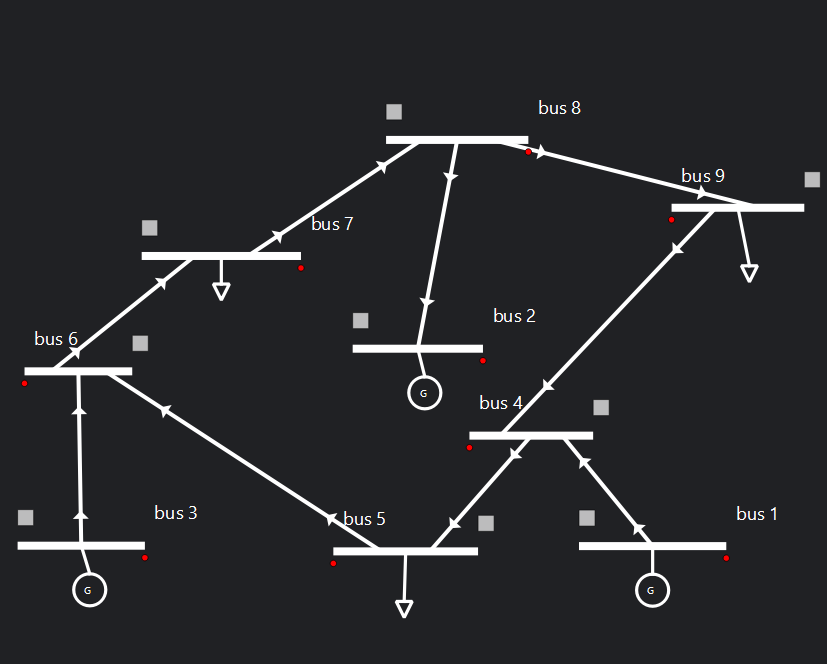
\includegraphics[width= 250 px]{Images/case9_topo.png}
  \caption{Schematic of the 9-bus grid.}
  \label{fig:case9topo}
\end{figure}

It can be seen in Figure~\ref{fig:9bus_error} that for such a small grid, there is not a significant difference between the different initialization options. The error evolution is very similar for all of them, and the error obtained is very close to the one obtained by Matpower, 
being the option without bound slacks slightly better as the vector of variables is considerably smaller. If there are no issues with the grid, the initialization with bound slacks is not necessary for this case.

\begin{figure}[!htb]
    \centering
    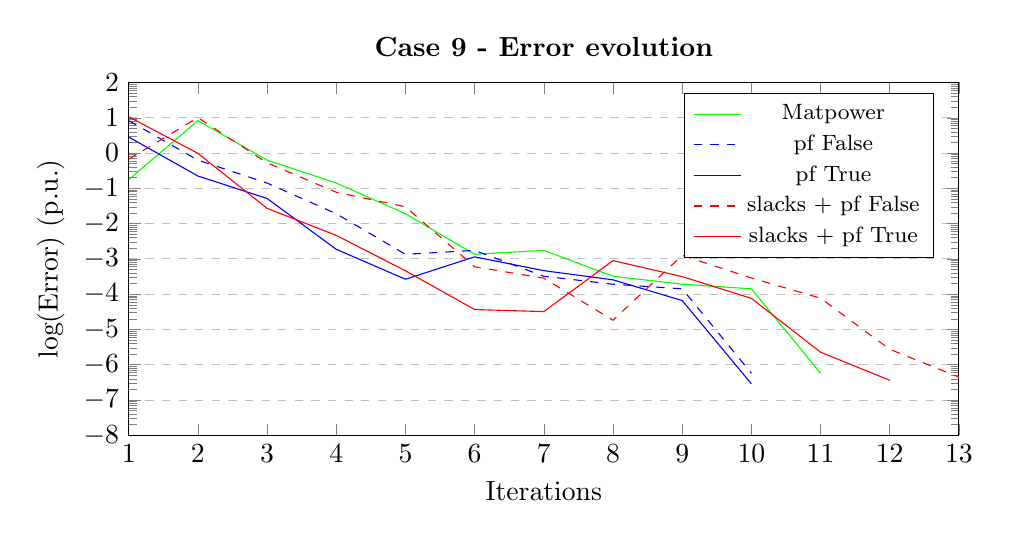
\begin{tikzpicture}
    \begin{semilogyaxis}[
        title={\textbf{Case 9 - Error evolution}},
        xlabel={Iterations},
        ylabel={log(Error) (p.u.)},
        width= \textwidth,
        height= 0.5\textwidth,
        xmin=1, xmax=13,
        ymin=1e-8, ymax=1e2,
        xtick={1,2,3,4,5,6,7,8,9,10,11,12,13},
        %ytick={1e-8,1e-6,1e-4,1e-2,1e0,1e2},
        log base 10 number format code/.code={\pgfmathprintnumber[fixed]{#1}},
        max space between ticks=20,
        legend pos=north east,
        ymajorgrids=true,
        grid style=dashed,
        scaled ticks=false,
        yticklabel style={/pgf/number format/sci},
        legend style={font=\footnotesize},        
    ]

    %Data for Matpower
    \addplot[
        color=green,
        mark=none,
        mark options={solid}
        ]
        coordinates {
        (1, 0.1765)
        (2, 8.305054238)
        (3, 0.630697772)
        (4, 0.141403676)
        (5, 0.019075407)
        (6, 0.001352357)
        (7, 0.001746417)
        (8, 0.000322236)
        (9, 0.000191987)
        (10, 0.000142097)
        (11, 5.75478E-07)
        };
        \addlegendentry{Matpower}

    % Data for 'pf False' plotted with dashed lines
    \addplot[
        color=blue,
        dashed,
        mark=none,
        mark options={dashed}
        ]
        coordinates {
        (1,8.305054238)(2,0.630697772)(3,0.141403676)(4,0.019075407)
        (5,0.001352357)(6,0.001746417)(7,0.000322236)(8,0.000191987)(9,0.000142097)
        (10,5.75e-07)
        };
        \addlegendentry{pf False}

    % Data for 'pf True'
    \addplot[
        color=blue,
        mark=none,
        mark options={solid}
        ]
        coordinates {
        (1,2.8442694)(2,0.224084957)(3,0.051708904)(4,0.001873459)
        (5,0.000265494)(6,0.001145971)(7,0.000464665)(8,0.00025553)(9,6.60e-05)
        (10,2.89e-07)
        };
        \addlegendentry{pf True}

    %Data for slacks + pf False
    \addplot[
        color=red,
        mark=none,
        dashed,
        mark options={dashed}
        ]
        coordinates {
    (1, 0.672594031)
    (2, 10.08607297)
    (3, 0.527802283)
    (4, 0.077601018)
    (5, 0.030048859)
    (6, 0.000599489)
    (7, 0.000284285)
    (8, 1.83E-05)
    (9, 0.001257839)
    (10, 0.000288391)
    (11, 7.69E-05)
    (12, 2.74E-06)
    (13, 4.47E-07)
        };
        \addlegendentry{slacks + pf False}

         %Data for slacks + pf True'
    \addplot[
        color=red,
        mark=none,
        mark options={solid}
        ]
        coordinates {
    (1, 10.69785291)
    (2, 0.981962281)
    (3, 0.027127147)
    (4, 0.004650334)
    (5, 0.000460963)
    (6, 3.68E-05)
    (7, 3.21E-05)
    (8, 0.000893703)
    (9, 0.0003156)
    (10, 7.62E-05)
    (11, 2.27E-06)
    (12, 3.64E-07)
        };
        \addlegendentry{slacks + pf True}

    \end{semilogyaxis}
    \end{tikzpicture}
    \caption{Error evolution for the Case 9 system for different initialization options.}
    \label{fig:9bus_error}
\end{figure}

The result can be visualized in GridCal's GUI as shown in Figure~\ref{fig:case9solved}.

\begin{figure}[H]
    \centering
    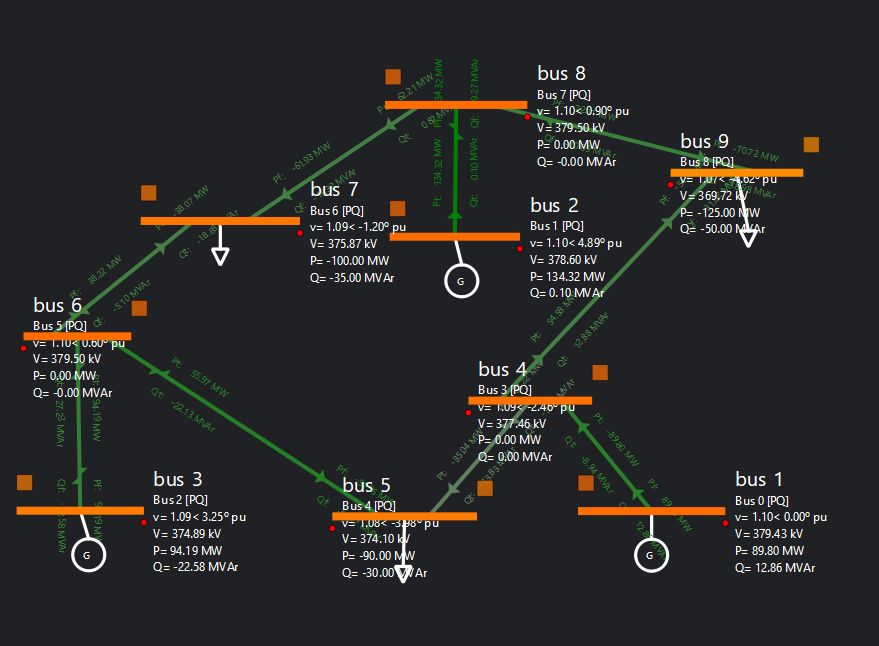
\includegraphics[width=250px]{Images/case9_solved.png}
    \caption{Plot of the solution of Case 9.}
    \label{fig:case9solved}
  \end{figure}

Something that can catch the eye is the orange color of the bus, which means they are near their upper voltage limit. This is due to the optimization trying to raise the voltage value as high as the limit allows
to reduce the current flowing through the lines, which reduces quadratically the losses. 

\subsubsection{Case Pegase89}

The next grid studied is a case with 89 buses obtained from the Pegase database \cite{josz2016ac}, with an interesting result shown in Figure~\ref{fig:peg89_error}.

%%%%%%%%%%%%%%%%%%%%%%%PEGASE89

\begin{figure}[H]
    \centering
    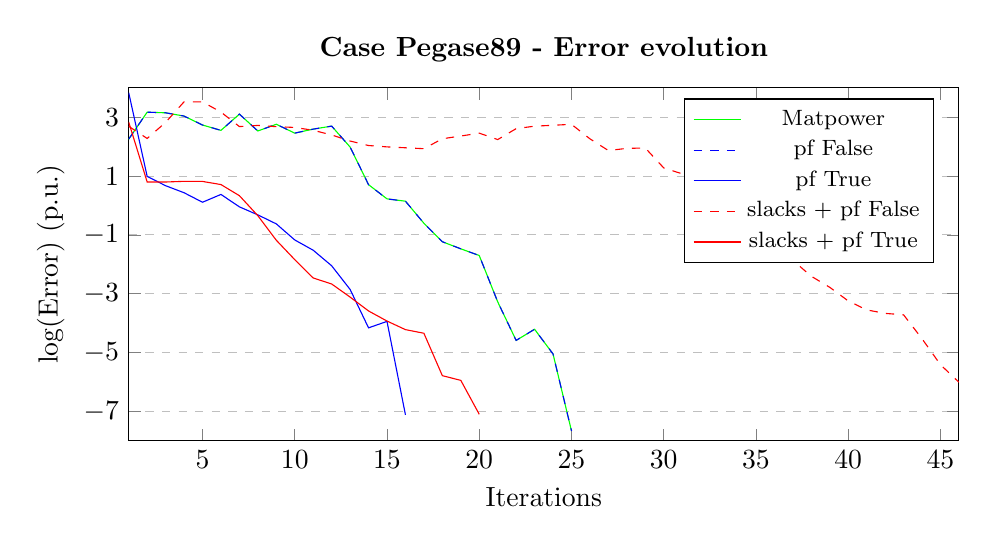
\begin{tikzpicture}
    \begin{semilogyaxis}[
        title={\textbf{Case Pegase89 - Error evolution}},
        xlabel={Iterations},
        ylabel={log(Error) (p.u.)},
        width=\textwidth,
        height=0.5\textwidth,
        xmin=1, xmax=46,
        ymin=1e-8, ymax=1e4,
        xtick={5,10,15,20,25,30,35,40,45},
        %ytick={1e-8,1e-6,1e-4,1e-2,1e0,1e2,1e4},
        log base 10 number format code/.code={\pgfmathprintnumber[fixed]{#1}},
        max space between ticks=20,
        legend pos=north east,
        ymajorgrids=true,
        grid style=dashed,
        scaled ticks=false,
        yticklabel style={/pgf/number format/sci},
        legend style={font=\footnotesize},        
    ]

    %Data for Matpower
    \addplot[
        color=green,
        mark=none,
        mark options={solid}
        ]
        coordinates {
            (0, 1.97E+02)
            (1, 1.81E+02)
            (2, 1.49E+03)
            (3, 1.42E+03)
            (4, 1.10E+03)
            (5, 5.45E+02)
            (6, 3.59E+02)
            (7, 1.28E+03)
            (8, 3.42E+02)
            (9, 5.79E+02)
            (10, 2.89E+02)
            (11, 3.96E+02)
            (12, 5.01E+02)
            (13, 9.73E+01)
            (14, 5.11E+00)
            (15, 1.68E+00)
            (16, 1.40E+00)
            (17, 2.49E-01)
            (18, 5.85E-02)
            (19, 3.36E-02)
            (20, 1.99E-02)
            (21, 5.30E-04)
            (22, 2.58E-05)
            (23, 6.17E-05)
            (24, 8.91E-06)
            (25, 2.15E-08)
            };
            \addlegendentry{Matpower}
    
    % Data for 'pf False' plotted with dashed lines
    \addplot[
        color=blue,
        dashed,
        mark=none,
        mark options={dashed}
        ]
        coordinates {
            (1, 180.6852809)
            (2, 1490.738444)
            (3, 1419.982727)
            (4, 1099.02207)
            (5, 545.1103587)
            (6, 358.905375)
            (7, 1279.15975)
            (8, 341.6215598)
            (9, 578.7692759)
            (10, 289.1161927)
            (11, 395.860816)
            (12, 501.3281398)
            (13, 97.33040695)
            (14, 5.1055572)
            (15, 1.678425193)
            (16, 1.40061097)
            (17, 0.24920242)
            (18, 0.058547064)
            (19, 0.0336216)
            (20, 0.019892455)
            (21, 0.000529315)
            (22, 2.58E-05)
            (23, 6.17E-05)
            (24, 8.91E-06)
            (25, 2.15E-08)
            
        };
        \addlegendentry{pf False}

    % Data for 'pf True'
    \addplot[
        color=blue,
        mark=none,
        mark options={solid}
        ]
        coordinates {
            (1, 6858.915797)
            (2, 9.777532171)
            (3, 4.710065804)
            (4, 2.71464747)
            (5, 1.290353948)
            (6, 2.378008759)
            (7, 0.89859405)
            (8, 0.47975603)
            (9, 0.236984468)
            (10, 0.067309606)
            (11, 0.030100396)
            (12, 0.008916589)
            (13, 0.001397848)
            (14, 6.90E-05)
            (15, 0.000114364)
            (16, 7.59E-08)
        };
        \addlegendentry{pf True}

    %Data for slacks + pf False
    \addplot[
        color=red,
        mark=none,
        dashed,
        mark options={dashed}
        ]
        coordinates {
            (1, 493.7519619)
            (2, 190.2715212)
            (3, 670.8818942)
            (4, 3358.316888)
            (5, 3337.824718)
            (6, 1504.864573)
            (7, 482.7699582)
            (8, 528.9254488)
            (9, 479.24423)
            (10, 451.0105948)
            (11, 361.3016494)
            (12, 250.3160809)
            (13, 155.626465)
            (14, 109.5497226)
            (15, 98.41240438)
            (16, 91.79191644)
            (17, 85.44510793)
            (18, 186.2518746)
            (19, 230.1803572)
            (20, 288.8504731)
            (21, 174.4224137)
            (22, 4.11E+02)
            (23, 4.99E+02)
            (24, 5.34E+02)
            (25, 5.77E+02)
            (26, 184.8406118)
            (27, 73.96119961)
            (28, 87.65671109)
            (29, 90.20320642)
            (30, 18.95713471)
            (31, 11.9277116)
            (32, 6.59372116)
            (33, 5.366626728)
            (34, 0.427055853)
            (35, 0.118797272)
            (36, 0.045138674)
            (37, 0.013643592)
            (38, 0.003908286)
            (39, 0.00164611)
            (40, 0.000568345)
            (41, 0.000281288)
            (42, 0.000214334)
            (43, 0.00019144)
            (44, 2.94E-05)
            (45, 3.85E-06)
            (46, 9.74E-07)               
        };
        \addlegendentry{slacks + pf False}

         %Data for slacks + pf True'
    \addplot[
        color=red,
        mark=none,
        mark options={solid}
        ]
        coordinates {
            (1, 687.0039266)
            (2, 6.308603441)
            (3, 6.291506138)
            (4, 6.630021909)
            (5, 6.581885519)
            (6, 5.149142934)
            (7, 2.157472908)
            (8, 0.450262838)
            (9, 0.065799541)
            (10, 0.014386682)
            (11, 0.003425975)
            (12, 0.00214243)
            (13, 0.000767392)
            (14, 0.00025888)
            (15, 0.00011754)
            (16, 6.00E-05)
            (17, 4.52E-05)
            (18, 1.63E-06)
            (19, 1.13E-06)
            (20, 7.93E-08)
        };
        \addlegendentry{slacks + pf True}

    \end{semilogyaxis}
    \end{tikzpicture}
    \caption{Error evolution for the Pegase89 system for different initialization options.}
    \label{fig:peg89_error}
\end{figure}

Firstly, it should be noted that the solution without bound slacks and with the power flow initialization disabled follows the exact same evolution as the Matpower solver. This did not happen in the previous case, but it seems to be due to the GridCal parser processing of the model.
For some cases during the developing of the software, some grids were unsolvable due to some of its parameters not being directly specified in the model. For instance, some line ratings were not specified, and while the Matpower solver would then ignore some of these limits,
the GridCal parser would not be able to process it in a correct way. To solve this, the parser has been adjusted to set a default value in case the lines are monitored but the rating is specified. Many other small nuances during the model loading could be
the source of this difference in the convergence.

The other relevant observation that can be done is that the power flow initialization is doing a great job in improving the convergence of the problem. In a real scenario situation, the user would input a grid model that is already in a feasible state, 
although it may not be optimal, but it might be close to what an optimum generation profile would be. In this case, the OPF using an initialization with power flow takes almost half of the iterations in the case without bound slacks, and a third in the case with bound slacks.

One last observation is that bound slacks are not useful in this case either. The error evolution is very similar to the one without bound slacks, and the number of variables is considerably larger, which will make the problem a bit heavier to run as it will be shown in a later subsection.

\subsubsection{Case 300}

The next case is a 300-bus system \cite{addibi1993power}, which is a considerably larger grid than the previous ones. The error evolution for each initialization is shown in Figure~\ref{fig:case300_error}.

%%%%%%%%%%%%%%%%%%%%%%%CASE 300


\begin{figure}[h]
    \centering
    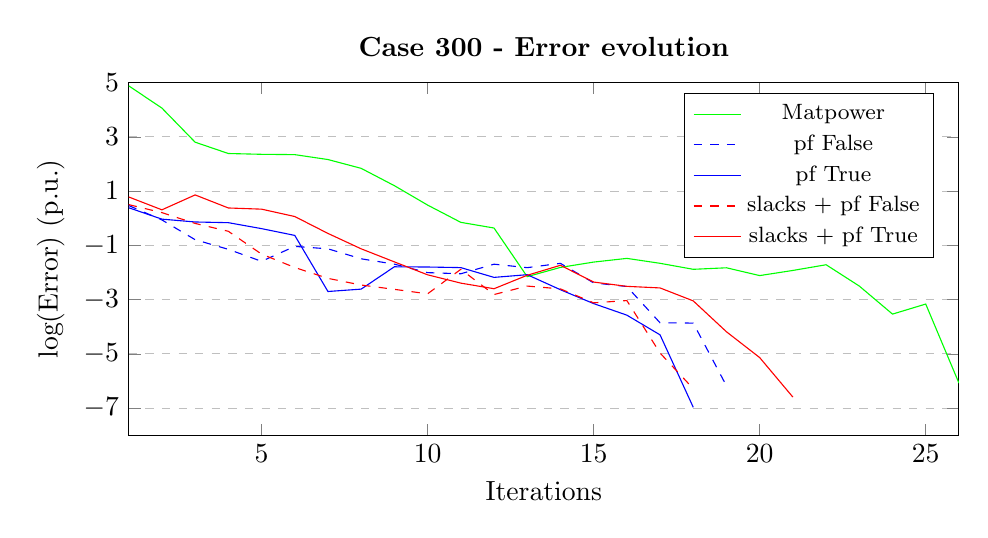
\begin{tikzpicture}
    \begin{semilogyaxis}[
        title={\textbf{Case 300 - Error evolution}},
        xlabel={Iterations},
        ylabel={log(Error) (p.u.)},
        width= \textwidth,
        height= 0.5\textwidth,
        xmin=1, xmax=26,
        ymin=1e-8, ymax=1e5,
        xtick={5,10,15,20,25},
        %ytick={1e-8,1e-6,1e-4,1e-2,1e0,1e2,1e4},
        log base 10 number format code/.code={\pgfmathprintnumber[fixed]{#1}},
        max space between ticks=20,
        legend pos=north east,
        ymajorgrids=true,
        grid style=dashed,
        scaled ticks=false,
        yticklabel style={/pgf/number format/sci},
        legend style={font=\footnotesize},        
    ]

    %Data for Matpower
    \addplot[
        color=green,
        mark=none,
        mark options={solid}
        ]
        coordinates {
            (1, 7.53E+04)
            (2, 1.14E+04)
            (3, 6.32E+02)
            (4, 2.42E+02)
            (5, 2.26E+02)
            (6, 2.20E+02)
            (7, 1.45E+02)
            (8, 6.87E+01)
            (9, 1.58E+01)
            (10, 3.05E+00)
            (11, 7.04E-01)
            (12, 4.35E-01)
            (13, 7.03E-03)
            (14, 1.54E-02)
            (15, 2.42E-02)
            (16, 3.31E-02)
            (17, 2.18E-02)
            (18, 1.31E-02)
            (19, 1.49E-02)
            (20, 7.69E-03)
            (21, 1.19E-02)
            (22, 1.93E-02)
            (23, 3.16E-03)
            (24, 2.93E-04)
            (25, 6.88E-04)
            (26, 8.43E-07)
            };
            \addlegendentry{Matpower}

    % Data for 'pf False' plotted with dashed lines
    \addplot[
        color=blue,
        dashed,
        mark=none,
        mark options={dashed}
        ]
        coordinates {
            (1, 2.936208787)
            (2, 0.863070361)
            (3, 0.161534637)
            (4, 0.071333199)
            (5, 0.025775797)
            (6, 0.091552775)
            (7, 0.07450434)
            (8, 0.031953639)
            (9, 0.020283202)
            (10, 0.009889533)
            (11, 0.008971603)
            (12, 0.020244771)
            (13, 0.015074886)
            (14, 0.021738874)
            (15, 0.004147349)
            (16, 0.003045018)
            (17, 0.000140213)
            (18, 0.000136692)
            (19, 6.64E-07)
            
        };
        \addlegendentry{pf False}

    % Data for 'pf True'
    \addplot[
        color=blue,
        mark=none,
        mark options={solid}
        ]
        coordinates {
            (1, 2.432229841)
            (2, 0.92458341)
            (3, 0.726214531)
            (4, 0.684812192)
            (5, 0.413152846)
            (6, 0.232583762)
            (7, 0.001993708)
            (8, 0.002440273)
            (9, 0.016226286)
            (10, 0.015922195)
            (11, 0.015141967)
            (12, 0.006602047)
            (13, 0.008294147)
            (14, 0.002318244)
            (15, 0.000714441)
            (16, 0.00026829)
            (17, 5.04E-05)
            (18, 1.08E-07)
            
        };
        \addlegendentry{pf True}

    %Data for slacks + pf False
    \addplot[
        color=red,
        mark=none,
        dashed,
        mark options={dashed}
        ]
        coordinates {
            (1, 3.167574855)
            (2, 1.603787928)
            (3, 0.642278168)
            (4, 0.329752885)
            (5, 0.047550026)
            (6, 0.015296491)
            (7, 0.006075237)
            (8, 0.003450498)
            (9, 0.002394262)
            (10, 0.00163828)
            (11, 0.013081511)
            (12, 0.001542913)
            (13, 0.003161681)
            (14, 0.002491171)
            (15, 0.00076242)
            (16, 0.000924757)
            (17, 1.08E-05) 
            (18, 5.23E-07)  
        };
        \addlegendentry{slacks + pf False}

         %Data for slacks + pf True'
    \addplot[
        color=red,
        mark=none,
        mark options={solid}
        ]
        coordinates {
            (1, 6.068166154)
            (2, 2.036464624)
            (3, 7.211447601)
            (4, 2.383818446)
            (5, 2.155179565)
            (6, 1.153516841)
            (7, 0.275017846)
            (8, 0.074454495)
            (9, 0.024604769)
            (10, 0.008204682)
            (11, 0.004061359)
            (12, 0.00252147)
            (13, 0.007900866)
            (14, 0.018418069)
            (15, 0.004443811)
            (16, 0.003086266)
            (17, 0.002698575)
            (18, 0.00089835)
            (19, 6.54E-05)
            (20, 7.33E-06)
            (21, 2.56E-07)
             
        };
        \addlegendentry{slacks + pf True}

    \end{semilogyaxis}
    \end{tikzpicture}
    \caption{Error evolution for the 300-bus system for different initialization options.}
    \label{fig:case300_error}
\end{figure}

The performance of the solver developed in this work outclasses the one of Matpower in this case. Considering that the solver is based on the same principles, this means that the GridCal modelled problem is better conditioned than the one modelled by Matpower,
which is why the solver has been developed in such an environment.

\subsubsection{Case GB}
Last case shown is a country-sized 2223-bus system that has been provided directly by Redeia, which models the Great Britain grid. Error evolutions are shown in Figure~\ref{fig:caseGB_error}.

%%%%%%%%%%%%%%%%%%%%%%%CASE GB


\begin{figure}[H]
    \centering
    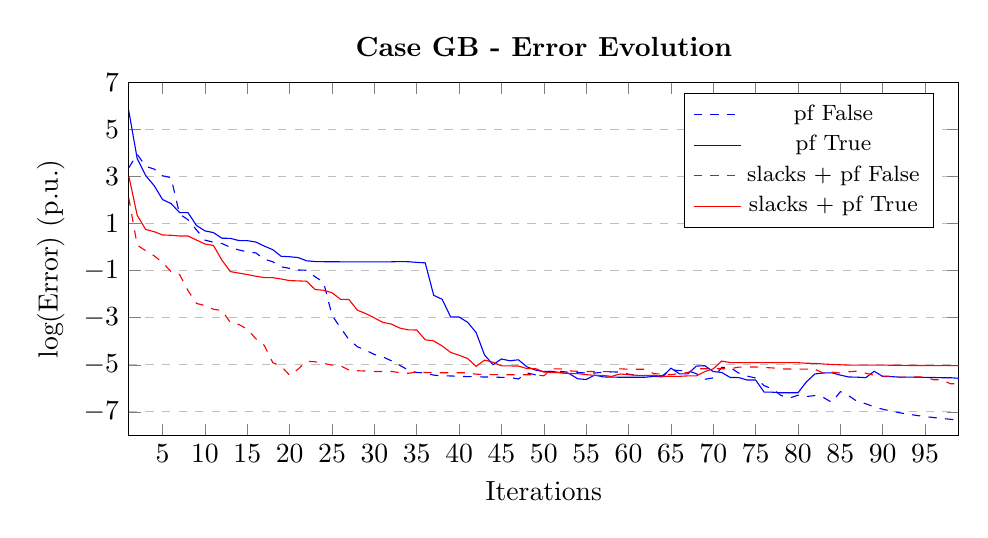
\begin{tikzpicture}
    \begin{semilogyaxis}[
        title={\textbf{Case GB - Error Evolution}},
        xlabel={Iterations},
        ylabel={log(Error) (p.u.)},
        width=\textwidth,
        height= 0.5\textwidth,
        xmin=1, xmax=99,
        ymin=1e-8, ymax=1e7,
        %xtick={10,20,30,40,50,60,70,80,90},
        %ytick={1e-8,1e-6,1e-4,1e-2,1e0,1e2,1e4,1e6},
        log base 10 number format code/.code={\pgfmathprintnumber[fixed]{#1}},
        max space between ticks=20,
        legend pos=north east,
        ymajorgrids=true,
        grid style=dashed,
        scaled ticks=false,
        yticklabel style={/pgf/number format/sci},
        legend style={font=\footnotesize},        
    ]

    % Data for 'pf False' plotted with dashed lines
    \addplot[
        color=blue,
        dashed,
        mark=none,
        mark options={dashed}
        ]
        coordinates {
            (1, 2352.813112)
            (2, 8928.483922)
            (3, 2734.583848)
            (4, 2091.219247)
            (5, 1083.581041)
            (6, 899.8106605)
            (7, 25.43791289)
            (8, 14.6163785)
            (9, 5.429096411)
            (10, 1.990894646)
            (11, 1.623204052)
            (12, 1.431413188)
            (13, 0.988402131)
            (14, 0.760754722)
            (15, 0.63180179)
            (16, 0.570487192)
            (17, 0.30913493)
            (18, 0.239603685)
            (19, 0.145910947)
            (20, 0.125213058)
            (21, 0.107168071)
            (22, 0.104320636)
            (23, 0.055052483)
            (24, 0.032543327)
            (25, 0.001261022)
            (26, 0.000374469)
            (27, 0.000116732)
            (28, 5.85E-05)
            (29, 4.10E-05)
            (30, 2.74E-05)
            (31, 2.17E-05)
            (32, 1.48E-05)
            (33, 9.42E-06)
            (34, 5.95E-06)
            (35, 4.68E-06)
            (36, 4.52E-06)
            (37, 3.63E-06)
            (38, 3.37E-06)
            (39, 3.35E-06)
            (40, 3.24E-06)
            (41, 3.12E-06)
            (42, 3.12E-06)
            (43, 3.01E-06)
            (44, 3.01E-06)
            (45, 2.92E-06)
            (46, 2.88E-06)
            (47, 2.49E-06)
            (48, 4.49E-06)
            (49, 3.78E-06)
            (50, 5.28E-06)
            (51, 5.26E-06)
            (52, 5.22E-06)
            (53, 4.78E-06)
            (54, 4.67E-06)
            (55, 4.50E-06)
            (56, 4.47E-06)
            (57, 4.81E-06)
            (58, 4.97E-06)
            (59, 4.94E-06)
            (60, 3.99E-06)
            (61, 3.50E-06)
            (62, 3.47E-06)
            (63, 3.46E-06)
            (64, 3.45E-06)
            (65, 6.08E-06)
            (66, 5.64E-06)
            (67, 5.53E-06)
            (68, 4.18E-06)
            (69, 2.42E-06)
            (70, 2.78E-06)
            (71, 7.69E-06)
            (72, 7.72E-06)
            (73, 4.43E-06)
            (74, 3.31E-06)
            (75, 2.74E-06)
            (76, 1.30E-06)
            (77, 9.35E-07)
            (78, 4.96E-07)
            (79, 3.88E-07)
            (80, 5.06E-07)
            (81, 4.48E-07)
            (82, 4.91E-07)
            (83, 4.07E-07)
            (84, 2.52E-07)
            (85, 7.20E-07)
            (86, 4.80E-07)
            (87, 2.75E-07)
            (88, 2.20E-07)
            (89, 1.63E-07)
            (90, 1.29E-07)
            (91, 1.07E-07)
            (92, 9.11E-08)
            (93, 7.94E-08)
            (94, 7.03E-08)
            (95, 6.31E-08)
            (96, 5.72E-08)
            (97, 5.23E-08)
            (98, 4.82E-08)
            (99, 4.47E-08)
            
        };
        \addlegendentry{pf False}

    % Data for 'pf True'
    \addplot[
        color=blue,
        mark=none,
        mark options={solid}
        ]
        coordinates {
            (1, 643178.5344)
            (2, 5900.292698)
            (3, 1106.700991)
            (4, 415.4098461)
            (5, 105.2807711)
            (6, 71.30182634)
            (7, 29.59955383)
            (8, 29.18531615)
            (9, 8.321889228)
            (10, 4.916244126)
            (11, 4.170715893)
            (12, 2.40607294)
            (13, 2.360678741)
            (14, 1.914702259)
            (15, 1.888603987)
            (16, 1.652948957)
            (17, 1.11008489)
            (18, 0.783511077)
            (19, 0.40843767)
            (20, 0.392203426)
            (21, 0.360863196)
            (22, 0.263150445)
            (23, 0.244530388)
            (24, 0.241226113)
            (25, 0.239070527)
            (26, 0.23851364)
            (27, 0.238473552)
            (28, 0.238473827)
            (29, 0.238469658)
            (30, 0.238469691)
            (31, 0.238469656)
            (32, 0.238469656)
            (33, 0.243976374)
            (34, 0.240570678)
            (35, 0.225341286)
            (36, 0.21569497)
            (37, 0.009008557)
            (38, 0.006080395)
            (39, 0.001082531)
            (40, 0.001072805)
            (41, 0.000644974)
            (42, 0.00023817)
            (43, 2.62E-05)
            (44, 1.01E-05)
            (45, 1.76E-05)
            (46, 1.48E-05)
            (47, 1.63E-05)
            (48, 8.21E-06)
            (49, 5.99E-06)
            (50, 5.03E-06)
            (51, 5.25E-06)
            (52, 4.56E-06)
            (53, 4.23E-06)
            (54, 2.54E-06)
            (55, 2.37E-06)
            (56, 3.64E-06)
            (57, 3.06E-06)
            (58, 2.98E-06)
            (59, 2.96E-06)
            (60, 2.96E-06)
            (61, 2.96E-06)
            (62, 2.96E-06)
            (63, 3.22E-06)
            (64, 3.06E-06)
            (65, 7.19E-06)
            (66, 4.12E-06)
            (67, 4.10E-06)
            (68, 8.77E-06)
            (69, 9.16E-06)
            (70, 5.15E-06)
            (71, 4.71E-06)
            (72, 2.89E-06)
            (73, 2.86E-06)
            (74, 2.26E-06)
            (75, 2.26E-06)
            (76, 6.93E-07)
            (77, 6.83E-07)
            (78, 6.47E-07)
            (79, 6.46E-07)
            (80, 6.44E-07)
            (81, 1.89E-06)
            (82, 4.08E-06)
            (83, 4.48E-06)
            (84, 4.56E-06)
            (85, 3.63E-06)
            (86, 3.03E-06)
            (87, 2.97E-06)
            (88, 2.83E-06)
            (89, 5.29E-06)
            (90, 3.20E-06)
            (91, 3.15E-06)
            (92, 2.98E-06)
            (93, 2.98E-06)
            (94, 2.96E-06)
            (95, 2.90E-06)
            (96, 2.88E-06)
            (97, 2.82E-06)
            (98, 2.82E-06)
            (99, 2.66E-06)
            
        };
        \addlegendentry{pf True}

    %Data for slacks + pf False
    \addplot[
        color=red,
        mark=none,
        dashed,
        mark options={dashed}
        ]
        coordinates {
            (1, 127.3283287)
            (2, 1.233341752)
            (3, 0.703699251)
            (4, 0.43017213)
            (5, 0.221907347)
            (6, 0.091207958)
            (7, 0.069120674)
            (8, 0.014185103)
            (9, 0.004054519)
            (10, 0.003296678)
            (11, 0.002286073)
            (12, 0.002032975)
            (13, 0.000624582)
            (14, 0.000515267)
            (15, 0.000326678)
            (16, 0.000128413)
            (17, 6.68E-05)
            (18, 1.23E-05)
            (19, 8.71E-06)
            (20, 3.57E-06)
            (21, 6.55E-06)
            (22, 1.41E-05)
            (23, 1.34E-05)
            (24, 1.14E-05)
            (25, 9.73E-06)
            (26, 9.10E-06)
            (27, 5.97E-06)
            (28, 5.58E-06)
            (29, 5.41E-06)
            (30, 5.20E-06)
            (31, 5.20E-06)
            (32, 5.20E-06)
            (33, 4.64E-06)
            (34, 4.34E-06)
            (35, 4.90E-06)
            (36, 4.69E-06)
            (37, 4.62E-06)
            (38, 4.59E-06)
            (39, 4.59E-06)
            (40, 4.58E-06)
            (41, 4.58E-06)
            (42, 3.99E-06)
            (43, 3.84E-06)
            (44, 3.81E-06)
            (45, 3.78E-06)
            (46, 3.76E-06)
            (47, 3.76E-06)
            (48, 3.76E-06)
            (49, 3.76E-06)
            (50, 3.41E-06)
            (51, 6.73E-06)
            (52, 6.72E-06)
            (53, 5.51E-06)
            (54, 5.27E-06)
            (55, 5.18E-06)
            (56, 5.15E-06)
            (57, 5.15E-06)
            (58, 5.15E-06)
            (59, 6.74E-06)
            (60, 6.46E-06)
            (61, 6.45E-06)
            (62, 6.45E-06)
            (63, 4.14E-06)
            (64, 4.12E-06)
            (65, 3.81E-06)
            (66, 4.22E-06)
            (67, 4.73E-06)
            (68, 6.83E-06)
            (69, 6.80E-06)
            (70, 6.80E-06)
            (71, 6.79E-06)
            (72, 6.79E-06)
            (73, 7.91E-06)
            (74, 8.06E-06)
            (75, 8.08E-06)
            (76, 7.69E-06)
            (77, 7.34E-06)
            (78, 6.66E-06)
            (79, 6.63E-06)
            (80, 6.60E-06)
            (81, 6.51E-06)
            (82, 6.49E-06)
            (83, 4.44E-06)
            (84, 4.87E-06)
            (85, 4.45E-06)
            (86, 5.02E-06)
            (87, 5.38E-06)
            (88, 4.37E-06)
            (89, 3.60E-06)
            (90, 3.32E-06)
            (91, 3.22E-06)
            (92, 2.94E-06)
            (93, 3.00E-06)
            (94, 3.03E-06)
            (95, 3.03E-06)
            (96, 2.31E-06)
            (97, 2.29E-06)
            (98, 1.56E-06)
            (99, 1.55E-06)
        };
        \addlegendentry{slacks + pf False}

         %Data for slacks + pf True'
    \addplot[
        color=red,
        mark=none,
        mark options={solid}
        ]
        coordinates {
        (1, 1091.229243)
        (2, 22.73981193)
        (3, 5.675467735)
        (4, 4.543233996)
        (5, 3.307131426)
        (6, 3.199128537)
        (7, 2.97460875)
        (8, 2.974125088)
        (9, 2.010558964)
        (10, 1.361382122)
        (11, 1.178734594)
        (12, 0.282020175)
        (13, 0.091440897)
        (14, 0.079111423)
        (15, 0.068560312)
        (16, 0.058161522)
        (17, 0.050883665)
        (18, 0.050581975)
        (19, 0.044334399)
        (20, 0.037813854)
        (21, 0.036831218)
        (22, 0.035580913)
        (23, 0.015837438)
        (24, 0.01468006)
        (25, 0.011571031)
        (26, 0.006077399)
        (27, 0.005921991)
        (28, 0.002086292)
        (29, 0.001488226)
        (30, 0.000981173)
        (31, 0.000635248)
        (32, 0.000539877)
        (33, 0.000363299)
        (34, 0.000305015)
        (35, 0.00030105)
        (36, 0.000115904)
        (37, 0.000103533)
        (38, 6.31E-05)
        (39, 3.36E-05)
        (40, 2.55E-05)
        (41, 1.85E-05)
        (42, 8.58E-06)
        (43, 1.58E-05)
        (44, 1.28E-05)
        (45, 9.00E-06)
        (46, 8.95E-06)
        (47, 8.83E-06)
        (48, 6.90E-06)
        (49, 6.90E-06)
        (50, 4.95E-06)
        (51, 4.63E-06)
        (52, 4.62E-06)
        (53, 4.25E-06)
        (54, 4.21E-06)
        (55, 3.80E-06)
        (56, 3.57E-06)
        (57, 3.53E-06)
        (58, 3.21E-06)
        (59, 4.06E-06)
        (60, 3.77E-06)
        (61, 3.57E-06)
        (62, 3.54E-06)
        (63, 3.52E-06)
        (64, 3.28E-06)
        (65, 3.23E-06)
        (66, 3.23E-06)
        (67, 3.37E-06)
        (68, 3.37E-06)
        (69, 5.13E-06)
        (70, 6.73E-06)
        (71, 1.44E-05)
        (72, 1.24E-05)
        (73, 1.24E-05)
        (74, 1.24E-05)
        (75, 1.24E-05)
        (76, 1.23E-05)
        (77, 1.23E-05)
        (78, 1.23E-05)
        (79, 1.23E-05)
        (80, 1.23E-05)
        (81, 1.16E-05)
        (82, 1.15E-05)
        (83, 1.08E-05)
        (84, 1.03E-05)
        (85, 1.00E-05)
        (86, 9.67E-06)
        (87, 9.66E-06)
        (88, 9.66E-06)
        (89, 9.66E-06)
        (90, 9.65E-06)
        (91, 9.57E-06)
        (92, 9.56E-06)
        (93, 9.34E-06)
        (94, 9.31E-06)
        (95, 9.28E-06)
        (96, 9.22E-06)
        (97, 9.17E-06)
        (98, 9.15E-06)
        (99, 9.15E-06)
             
        };
        \addlegendentry{slacks + pf True}
    \end{semilogyaxis}
    \end{tikzpicture}
    \caption{Error evolution for the Great Britain grid for different initialization options.}
    \label{fig:caseGB_error}
\end{figure}

In this case, there is no comparative with the Matpower solver since the data is stored in a file that can only be managed in GridCal, and the model is not public. The results show a really promising evolution for a real use case,
obtaining a low error in a few iterations. The slack initialization option can be preferred in this case, which is to be expected since it is a case that has not been tested before, and it might correspond 
to a difficult grid state (meaning the limits could be a bit strict, some generators/lines could be disabled or the load profile could be high).

Despite the good performance during the first steps, it stagnates when asking for lower tolerance values, a side effect of adding a lot of variables to the problem.


\subsection{Effect of tap variables control - Case IEEE14}

Once having seen the performance of the solver in some study cases, it is time to analyze the effect of the tap variables control. This control is a feature that allows the solver to manage the tap variables of the transformers in the grid, 
which are the ones that can be modified to control the voltage levels or the power transfer. This control can be done in two ways: by setting the tap variables as fixed variables or by setting them as optimization variables. The first option is the one 
that has been used in the previous subsections, and the second one is the one that is going to be tested in this one.

The grid used is the IEEE14 model grid \cite{dabbagchi1993power}, which is a 14-bus grid that includes transformers. Firstly, the error evolution is compared in Figures~\ref{fig:case14_error} and~\ref{fig:case14_tap_error} to see the effect of adding this tap variables. 

%%%% CASE14 normal

\begin{figure}[H]
    \centering
    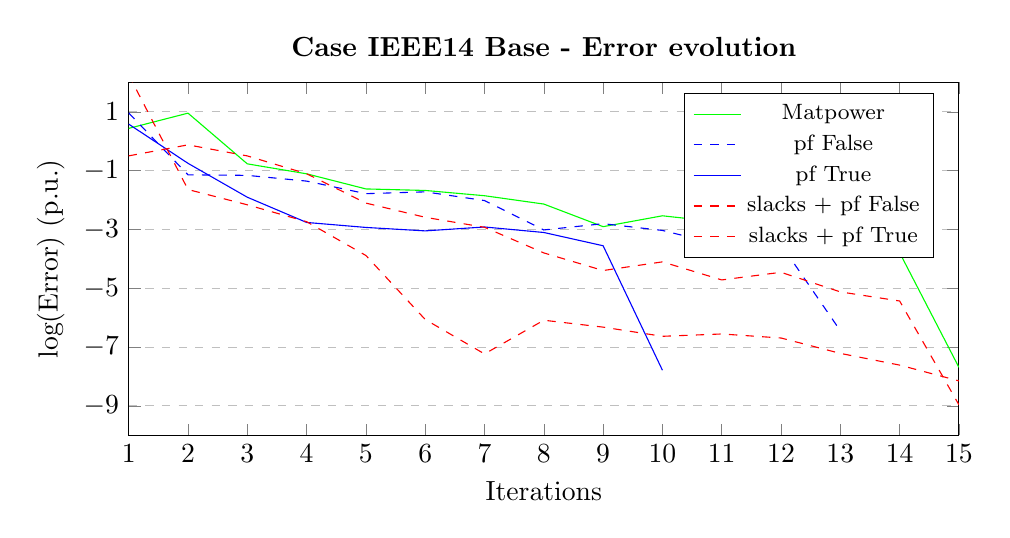
\begin{tikzpicture}
    \begin{semilogyaxis}[
        title={\textbf{Case IEEE14 Base - Error evolution}},
        xlabel={Iterations},
        ylabel={log(Error) (p.u.)},
        width=\textwidth,
        height= 0.5\textwidth,
        xmin=1, xmax=15,
        ymin=1e-10, ymax=1e2,
        log base 10 number format code/.code={\pgfmathprintnumber[fixed]{#1}},
        max space between ticks=20,
        legend pos=north east,
        ymajorgrids=true,
        grid style=dashed,
        scaled ticks=false,
        yticklabel style={/pgf/number format/sci},
        legend style={font=\footnotesize},        
    ]

    %Data for Matpower'
    \addplot[
        color=green,
        mark=none,
        mark options={solid}
        ]
        coordinates {
            (1, 2.75E+00)
            (2, 9.07E+00)
            (3, 1.71E-01)
            (4, 7.85E-02)
            (5, 2.40E-02)
            (6, 2.13E-02)
            (7, 1.41E-02)
            (8, 7.34E-03)
            (9, 1.25E-03)
            (10, 2.93E-03)
            (11, 1.76E-03)
            (12, 5.51E-04)
            (13, 6.50E-04)
            (14, 1.63E-04)
            (15, 2.05E-08)
        };
        \addlegendentry{Matpower}

    % Data for 'pf False' plotted with dashed lines
    \addplot[
        color=blue,
        dashed,
        mark=none,
        mark options={dashed}
        ]
        coordinates {
            (1, 9.213751716)
            (2, 0.072540437)
            (3, 0.069420068)
            (4, 0.044297854)
            (5, 0.016550251)
            (6, 0.019103711)
            (7, 0.009657606)
            (8, 0.000967572)
            (9, 0.001577085)
            (10, 0.000931124)
            (11, 0.000296858)
            (12, 0.000308507)
            (13, 3.61E-07)
            
        };
        \addlegendentry{pf False}

    % Data for 'pf True'
    \addplot[
        color=blue,
        mark=none,
        mark options={solid}
        ]
        coordinates {
            (1, 3.8416754)
            (2, 0.178257865)
            (3, 0.01254553)
            (4, 0.001738809)
            (5, 0.00117642)
            (6, 0.000898434)
            (7, 0.001219247)
            (8, 0.000792423)
            (9, 0.000280386)
            (10, 1.64E-08)
            
        };
        \addlegendentry{pf True}

    %Data for slacks + pf False
    \addplot[
        color=red,
        mark=none,
        dashed,
        mark options={dashed}
        ]
        coordinates {
            (1, 0.319744701)
            (2, 0.757329267)
            (3, 0.318402463)
            (4, 0.07900032)
            (5, 0.007922032)
            (6, 0.002602126)
            (7, 0.001190353)
            (8, 0.000160066)
            (9, 4.03E-05)
            (10, 7.94E-05)
            (11, 1.93E-05)
            (12, 3.51E-05)
            (13, 7.56E-06)
            (14, 3.71E-06)
            (15, 1.09E-09)
        };
        \addlegendentry{slacks + pf False}

    %Data for slacks + pf True
    \addplot[
        color=red,
        mark=none,
        dashed,
        mark options={dashed}
        ]
        coordinates {
            (1, 181.62441022700224)
            (2, 0.022897458206679974)
            (3, 0.006929041774338571)
            (4, 0.0018469169615173621)
            (5, 0.00013061962618515609)
            (6, 8.69767199952891e-07)
            (7, 5.8733757965589416e-08)
            (8, 8.222145107797376e-07)
            (9, 4.788624543636417e-07)
            (10, 2.3350350384465183e-07)
            (11, 2.8026613489491764e-07)
            (12, 2.0436953128261232e-07)
            (13, 6.124936153067041e-08)
            (14, 2.4486406772230067e-08)
            (15, 7.11319596670143e-09)
            (16, 7.80715019464817e-11)
        };
        \addlegendentry{slacks + pf True}
        
    \end{semilogyaxis}
    \end{tikzpicture}
    \caption{Error evolution for the Case IEEE14 for different initialization options.}
    \label{fig:case14_error}
\end{figure}


%%%% CASE14 taps

\begin{figure}[H]
    \centering
    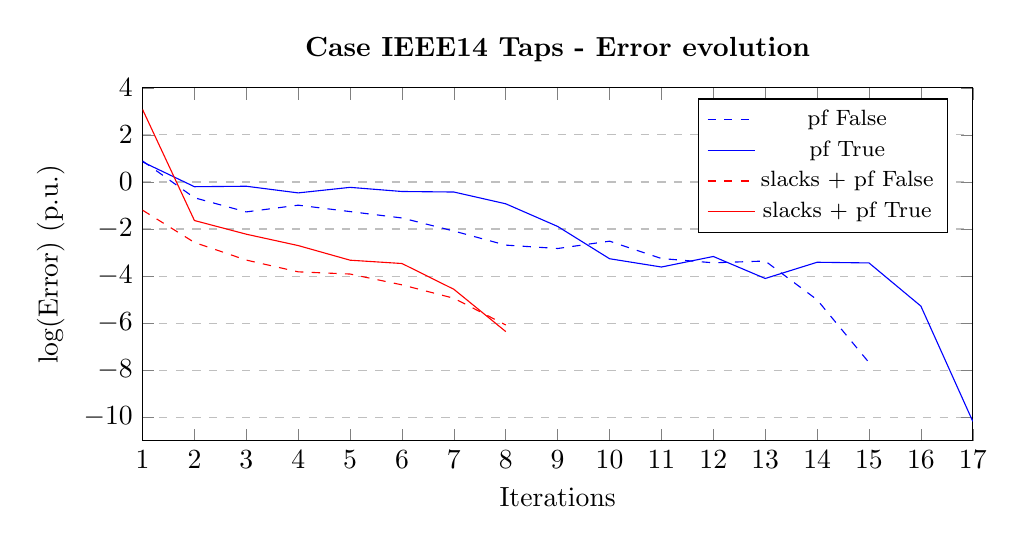
\begin{tikzpicture}
    \begin{semilogyaxis}[
        title={\textbf{Case IEEE14 Taps - Error evolution}},
        xlabel={Iterations},
        ylabel={log(Error) (p.u.)},
        width=\textwidth,
        height= 0.5\textwidth,
        xmin=1, xmax=17,
        ymin=1e-11, ymax=1e4,
        log base 10 number format code/.code={\pgfmathprintnumber[fixed]{#1}},
        max space between ticks=20,
        legend pos=north east,
        ymajorgrids=true,
        grid style=dashed,
        scaled ticks=false,
        yticklabel style={/pgf/number format/sci},
        legend style={font=\footnotesize},        
    ]

    % Data for 'pf False' plotted with dashed lines
    \addplot[
        color=blue,
        dashed,
        mark=none,
        mark options={dashed}
        ]
        coordinates {
            (1, 7.859900967)
            (2, 0.212772372)
            (3, 0.053400402)
            (4, 0.103219542)
            (5, 0.055136853)
            (6, 0.029458721)
            (7, 0.008210894)
            (8, 0.002070377)
            (9, 0.001485723)
            (10, 0.003043214)
            (11, 0.000556424)
            (12, 0.000366643)
            (13, 0.000436105)
            (14, 9.82E-06)
            (15, 2.10E-08)
        };
        \addlegendentry{pf False}

    % Data for 'pf True'
    \addplot[
        color=blue,
        mark=none,
        mark options={solid}
        ]
        coordinates {
            (1, 7.128524175)
            (2, 0.62936423)
            (3, 0.658239697)
            (4, 0.343270231)
            (5, 0.590285754)
            (6, 0.393917972)
            (7, 0.374122739)
            (8, 0.118023825)
            (9, 0.0128761)
            (10, 0.000546211)
            (11, 0.000242559)
            (12, 0.000679994)
            (13, 7.90E-05)
            (14, 0.000386629)
            (15, 0.00036193)
            (16, 5.28E-06)
            (17, 6.66E-11)
        };
        \addlegendentry{pf True}

    %Data for slacks + pf False
    \addplot[
        color=red,
        mark=none,
        dashed,
        mark options={dashed}
        ]
        coordinates {
            (1, 0.063322094)
            (2, 0.002683596)
            (3, 0.000477475)
            (4, 0.000151315)
            (5, 0.000122007)
            (6, 4.23E-05)
            (7, 1.14E-05)
            (8, 8.33E-07)
        };
        \addlegendentry{slacks + pf False}

         %Data for slacks + pf True'
    \addplot[
        color=red,
        mark=none,
        mark options={solid}
        ]
        coordinates {
            (1, 1210.715673)
            (2, 0.022978507)
            (3, 0.00602)
            (4, 0.001979625)
            (5, 0.000473052)
            (6, 0.000341739)
            (7, 2.74E-05)
            (8, 4.37E-07)
        };
        \addlegendentry{slacks + pf True}
    \end{semilogyaxis}
    \end{tikzpicture}
    \caption{Error evolution for the Case IEEE14 with tap variables for different initialization options.}
    \label{fig:case14_tap_error}
\end{figure}

There are two important remarks obtained from these error evolutions. Firstly, the case is solved in fewer iterations in the version of the solver developed in this project. Secondly, the usage of bound slacks improves convergence for the case with tap variables.
A more detailed analysis is done for the solution values for this case to analyze the impact of adding new optimization variables. For simplicity, the comparison will be made only for the cases with power flow initialization and without bound slacks, 
as they add to the cost function and the interest of this analysis is just testing the effect of using tap optimization.

Figures~\ref{fig:v_14} and~\ref{fig:gen_14} show the values of the solution for the bus voltages and generators. Note that there are no differences between the case solved with Matpower and the developed software.
The case with controlled tap variable has some slight differences, specially regarding the voltage magnitude. The impact in the generation is also noticeable for the reactive power generation, which has shifted mostly from generator 1 to generator 3.


\begin{figure}[H]
    \begin{minipage}{0.5\textwidth}
        \centering
        % Voltage Angles Plot
        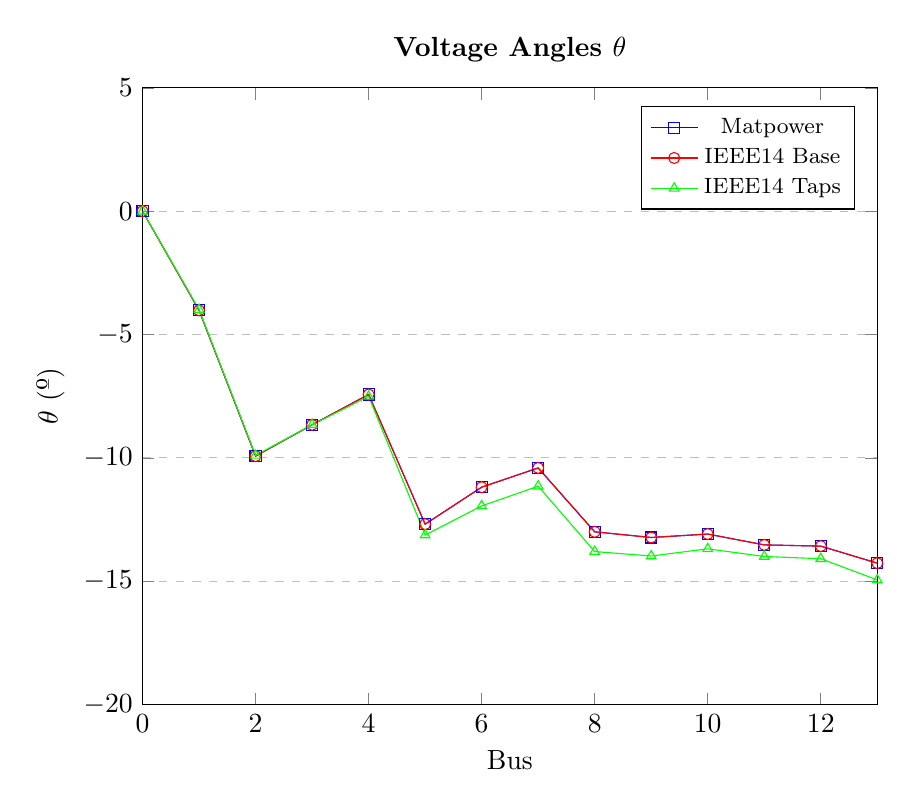
\begin{tikzpicture}
        \begin{axis}[
            title={\textbf{Voltage Angles $\theta$}},
            xlabel={Bus},
            ylabel={$\theta$ (º)},
            width = 0.9\textwidth,
            xmin=0, xmax=13,
            ymin=-20, ymax=5,
            xtick={0,2,4,6,8,10,12},
            ytick={-20,-15,-10,-5,0,5},
            legend pos=north east,
            legend style = {font = \footnotesize},
            ymajorgrids=true,
            grid style=dashed,
        ]

        \addplot[
            color=blue,
            mark=square,
            ]
            coordinates {
            (0,0.00) (1,-4.02) (2,-9.93) (3,-8.66) (4,-7.43) (5,-12.69) (6,-11.19) (7,-10.41) (8,-13.00) (9,-13.23) (10,-13.09) (11,-13.53) (12,-13.58) (13,-14.27)
            };
            \addlegendentry{Matpower}

        \addplot[
            color=red,
            mark=o,
            ]
            coordinates {
            (0,0.00) (1,-4.02) (2,-9.93) (3,-8.66) (4,-7.43) (5,-12.69) (6,-11.19) (7,-10.41) (8,-13.00) (9,-13.23) (10,-13.09) (11,-13.53) (12,-13.58) (13,-14.27)
            };
            \addlegendentry{IEEE14 Base}

        \addplot[
            color=green,
            mark=triangle,
            ]
            coordinates {
            (0,0.00) (1,-3.99) (2,-9.90) (3,-8.66) (4,-7.51) (5,-13.13) (6,-11.95) (7,-11.15) (8,-13.80) (9,-13.98) (10,-13.69) (11,-14.00) (12,-14.09) (13,-14.95)
            };
            \addlegendentry{IEEE14 Taps}
        \end{axis}
        \end{tikzpicture}
    \end{minipage}\hfill
    \begin{minipage}{0.5\textwidth}
        \centering
        % Voltage Magnitudes Plot
        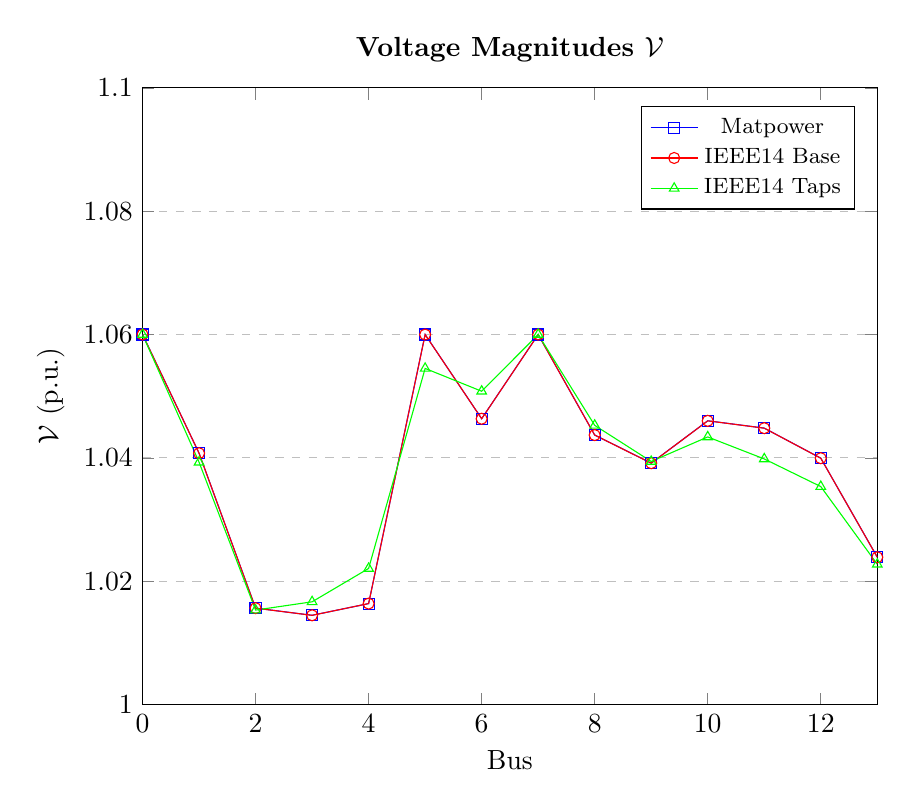
\begin{tikzpicture}
        \begin{axis}[
            title={\textbf{Voltage Magnitudes $\mathcal{V}$}},
            xlabel={Bus},
            ylabel={$\mathcal{V}$ (p.u.)},
            width=0.9\textwidth,
            xmin=0, xmax=13,
            ymin=1.0, ymax=1.1,
            xtick={0,2,4,6,8,10,12},
            ytick={1.00,1.02,1.04,1.06,1.08,1.10},
            legend pos=north east,
            legend style = {font = \footnotesize},
            ymajorgrids=true,
            grid style=dashed,
        ]

        \addplot[
            color=blue,
            mark=square,
            ]
            coordinates {
            (0,1.06000) (1,1.04075) (2,1.01563) (3,1.01446) (4,1.01636) (5,1.06000) (6,1.04635) (7,1.06000) (8,1.04370) (9,1.03914) (10,1.04601) (11,1.04482) (12,1.03995) (13,1.02389)
            };
            \addlegendentry{Matpower}

        \addplot[
            color=red,
            mark=o,
            ]
            coordinates {
            (0,1.06000) (1,1.04075) (2,1.01562) (3,1.01446) (4,1.01636) (5,1.05999) (6,1.04634) (7,1.05999) (8,1.04369) (9,1.03913) (10,1.04600) (11,1.04481) (12,1.03994) (13,1.02388)
            };
            \addlegendentry{IEEE14 Base}

        \addplot[
            color=green,
            mark=triangle,
            ]
            coordinates {
            (0,1.06000) (1,1.03929) (2,1.01531) (3,1.01665) (4,1.02206) (5,1.05450) (6,1.05080) (7,1.06000) (8,1.04527) (9,1.03941) (10,1.04339) (11,1.03982) (12,1.03534) (13,1.02274)
            };
            \addlegendentry{IEEE14 Taps}

        \end{axis}
        \end{tikzpicture}
    \end{minipage}
    \caption{Voltage comparison for the Case IEEE14 considering tap variables.}
    \label{fig:v_14}
\end{figure}


\begin{figure}[H]
    \begin{minipage}{0.5\textwidth}
        \centering

        % P (MW) Bar Graph
        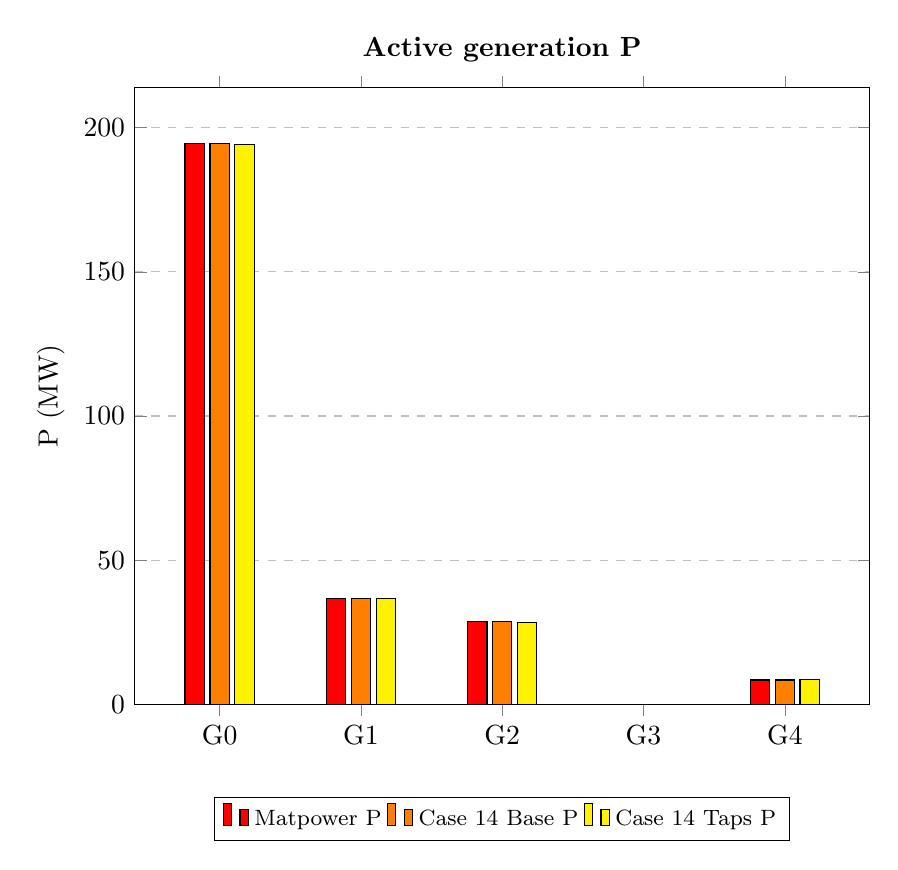
\begin{tikzpicture}
        \begin{axis}[
            title={\textbf{Active generation P}},
            ybar,
            enlarge x limits=0.15,
            ymin=0,
            width=0.9\textwidth,
            legend style={at={(0.5,-0.15)},
            anchor=north,legend columns=-1, font=\footnotesize},
            ylabel={P (MW)},
            symbolic x coords={G0,G1,G2,G3,G4},
            xtick=data,
            nodes near coords align={vertical},
            bar width=7pt,
            ymajorgrids,
            grid style=dashed,
        ]
        \addplot[fill=red]
            coordinates {(G0,194.33) (G1,36.72) (G2,28.74) (G3,0.00) (G4,8.50)};
        \addplot[fill=orange]
            coordinates {(G0,194.33) (G1,36.72) (G2,28.74) (G3,0.00) (G4,8.49)};
        \addplot[fill=yellow]
            coordinates {(G0,194.24) (G1,36.70) (G2,28.46) (G3,0.00) (G4,8.81)};
        
        \legend{Matpower P,Case 14 Base P,Case 14 Taps P}
        \end{axis}
        \end{tikzpicture}
    \end{minipage}\hfill
    \begin{minipage}{0.5\textwidth}
        \centering

        % Q (Mvar) Bar Graph
        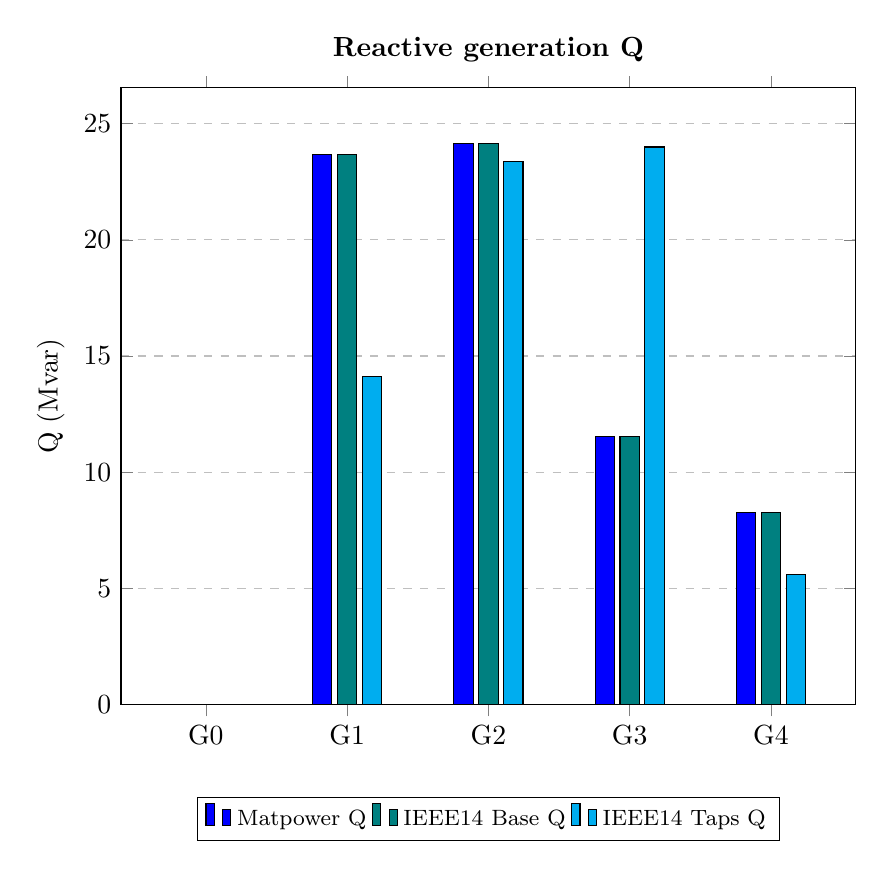
\begin{tikzpicture}
        \begin{axis}[
             title={\textbf{Reactive generation Q}},
            ybar,
            enlarge x limits=0.15,
            ymin=0,
            width=0.9\textwidth,
            legend style={at={(0.5,-0.15)},
            anchor=north,legend columns=-1, font=\footnotesize},
            ylabel={Q (Mvar)},
            symbolic x coords={G0,G1,G2,G3,G4},
            xtick=data,
            nodes near coords align={vertical},
            bar width=7pt,
            ymajorgrids,
            grid style = dashed,
        ]
        \addplot[fill=blue]
            coordinates {(G0,0.00) (G1,23.69) (G2,24.13) (G3,11.55) (G4,8.27)};
        \addplot[fill=teal]
            coordinates {(G0,0.01) (G1,23.68) (G2,24.13) (G3,11.54) (G4,8.27)};
        \addplot[fill=cyan]
            coordinates {(G0,0.00) (G1,14.11) (G2,23.37) (G3,24.00) (G4,5.60)};
        
        \legend{Matpower Q, IEEE14 Base Q, IEEE14 Taps Q}
        \end{axis}
        \end{tikzpicture}
\end{minipage}
    \caption{Generation comparison for Case IEEE14.}
    \label{fig:gen_14}
\end{figure}

Table~\ref{tab:tap_setpoints} shows the setpoints for the tap variables of the transformers in the grid as obtained with the solver developed. Note that the transformers that only have one variable controlled have a $N/C$ (Non-Controlled) as a solution.

\begin{table}[H]
    \centering
    \caption{Tap variable setpoints for the transformers of the corresponding branches in IEEE14.}
    \begin{tabular}{lcc}
    \hline
    \textbf{Controlled trafos} & \textbf{m\_p (p.u)} & \textbf{$\tau$ (º)} \\ \hline\hline
    Branch 17                  & 0.965876            & 0.754872          \\ 
    Branch 18                  & N/C                 & 1.365530          \\ 
    Branch 19                  & 0.974728            & N/C                \\ \hline
    \end{tabular}
    
    \label{tab:tap_setpoints}
\end{table}

The important result is shown in Table~\ref{tab:costs_tap}, which shows the impact of being able to control the tap variables setpoints in the cost of operation. Of course, this impact may not seem big in this case, representing
a reduction of cost of only 0.03\%. However, this result has only considered a small grid, without using properly modelled generation costs, and only controlling three transformers. And still, considering the total expenses of a country-sized grid as well as this result
being an instant photo of a given grid state, it can translate in substantial savings in the long-term. 

\begin{table}[H]
    \centering
    \caption{Comparison of costs between different cases.}
    \begin{tabular}{lccc}
    \hline
                          & \textbf{Matpower} & \textbf{Case 14 Base} & \textbf{Case 14 Taps} \\ \hline\hline
    \textbf{Cost (€/MWh)} & 8081.53           & 8081.53                  & 8078.85               \\ \hline
    \end{tabular}
    \label{tab:costs_tap}
    \end{table}
    

\subsection{Effect of reactive control}

Using the same base case, now the test is performed over the reactive power control. The limit is set as a maximum of a power factor of 0.8, which is translated to a maximum reactive power generation of 75\% of the active power generation.
The constraint is applied with respect to the absolute value of Q, meaning this constraint applies to both the injection and consumption of reactive power. Figure~\ref{fig:ctQ_V} shows the effect in the voltage values. There is a noticeable drop in magnitude in some of the buses.

\begin{figure}[!htb]
    \begin{minipage}{0.5\textwidth}
        \centering
        % Voltage Angles Plot
        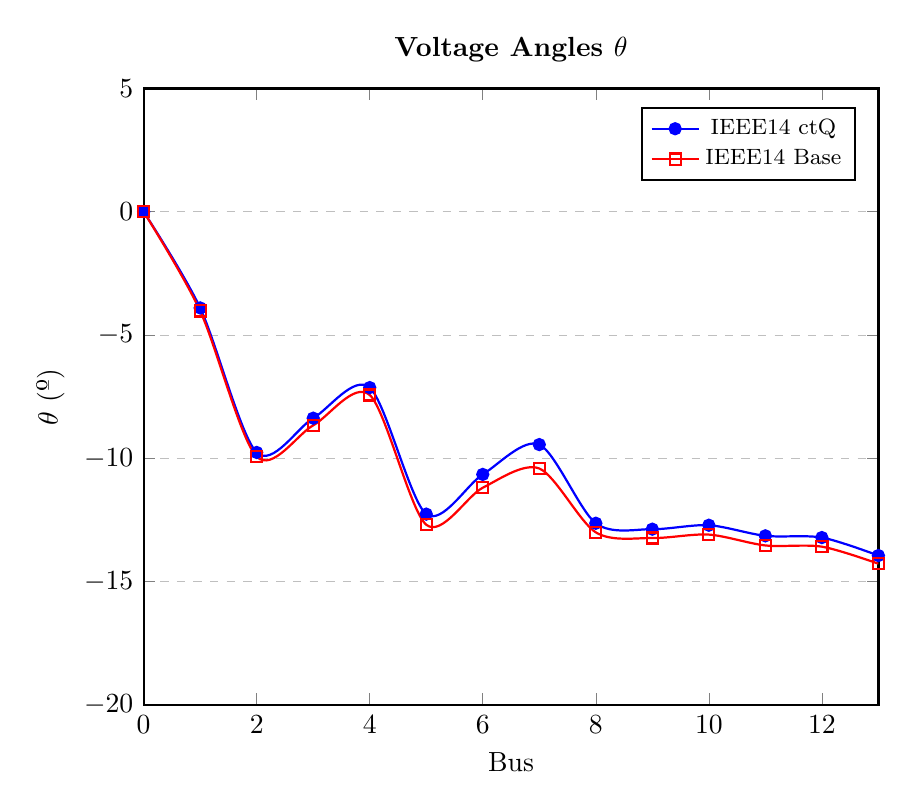
\begin{tikzpicture}
        \begin{axis}[
            title={\textbf{Voltage Angles $\theta$}},
            width=0.9\textwidth,
            xlabel={Bus},
            ylabel={$\theta$ (º)},
            xmin=0, xmax=13,
            ymin=-20, ymax=5,
            legend pos=north east,
            ymajorgrids=true,
            grid style=dashed,
            thick,
            legend style={font=\footnotesize},
        ]
        % Case 14 ctQ - Va
        \addplot[
            color=blue,
            mark=*,
            smooth,
            ]
            coordinates {
            (0,0.00) (1,-3.90) (2,-9.76) (3,-8.37) (4,-7.13) (5,-12.26) (6,-10.65) (7,-9.44) (8,-12.63) (9,-12.87) (10,-12.71) (11,-13.14) (12,-13.21) (13,-13.94)
            };
            \addlegendentry{IEEE14 ctQ}

        % Case 14 Base - Theta
        \addplot[
            color=red,
            mark=square,
            smooth,
            ]
            coordinates {
            (0,0.00) (1,-4.02) (2,-9.93) (3,-8.66) (4,-7.43) (5,-12.69) (6,-11.19) (7,-10.41) (8,-13.00) (9,-13.23) (10,-13.09) (11,-13.53) (12,-13.58) (13,-14.27)
            };
            \addlegendentry{IEEE14 Base}
        \end{axis}
        \end{tikzpicture}
    \end{minipage}\hfill
    \begin{minipage}{0.5\textwidth}
        \centering
        % Voltage Magnitudes Plot
        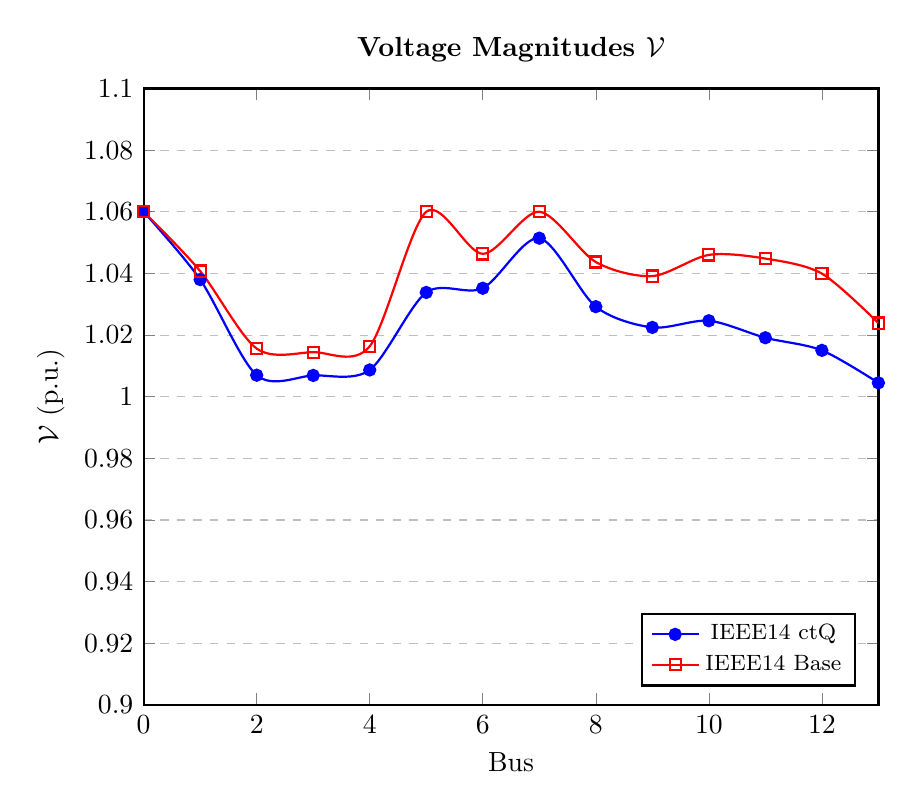
\begin{tikzpicture}
        \begin{axis}[
            title={\textbf{Voltage Magnitudes $\mathcal{V}$}},
            width=0.9\textwidth,
            xlabel={Bus},
            ylabel={$\mathcal{V}$ (p.u.)},
            xmin=0, xmax=13,
            ymin=0.9, ymax=1.1,
            legend pos=south east,
            ymajorgrids=true,
            grid style=dashed,
            thick,
            legend style={font=\footnotesize},
        ]

        % Case 14 ctQ - Vm
        \addplot[
            color=blue,
            mark=*,
            smooth,
            ]
            coordinates {
            (0,1.06000) (1,1.03800) (2,1.00698) (3,1.00691) (4,1.00868) (5,1.03382) (6,1.03519) (7,1.05143) (8,1.02921) (9,1.02248) (10,1.02464) (11,1.01913) (12,1.01504) (13,1.00450)
            };
            \addlegendentry{IEEE14 ctQ}

        % Case 14 Base - v
        \addplot[
            color=red,
            mark=square,
            smooth,
            ]
            coordinates {
            (0,1.06000) (1,1.04075) (2,1.01562) (3,1.01446) (4,1.01636) (5,1.05999) (6,1.04634) (7,1.05999) (8,1.04369) (9,1.03913) (10,1.04600) (11,1.04481) (12,1.03994) (13,1.02388)
            };
            \addlegendentry{IEEE14 Base}
        \end{axis}
        \end{tikzpicture}
    \end{minipage}
    \caption{Voltage comparison for the Case IEEE14 with and without reactive control.}
    \label{fig:ctQ_V}
\end{figure}


In Figure~\ref{fig:ctQ_gen}, it can be seen that generator 2, which previously had a reactive generation of 24.12 Mvar, now has a generation of 20.96 Mvar, which corresponds exactly to the 75\% of the active power generation.
This generator being at its limit for reactive power generation means the other generator have to contribute to reactive generation, impacting the voltage levels in the grid.

\begin{figure}[H]
    \centering
    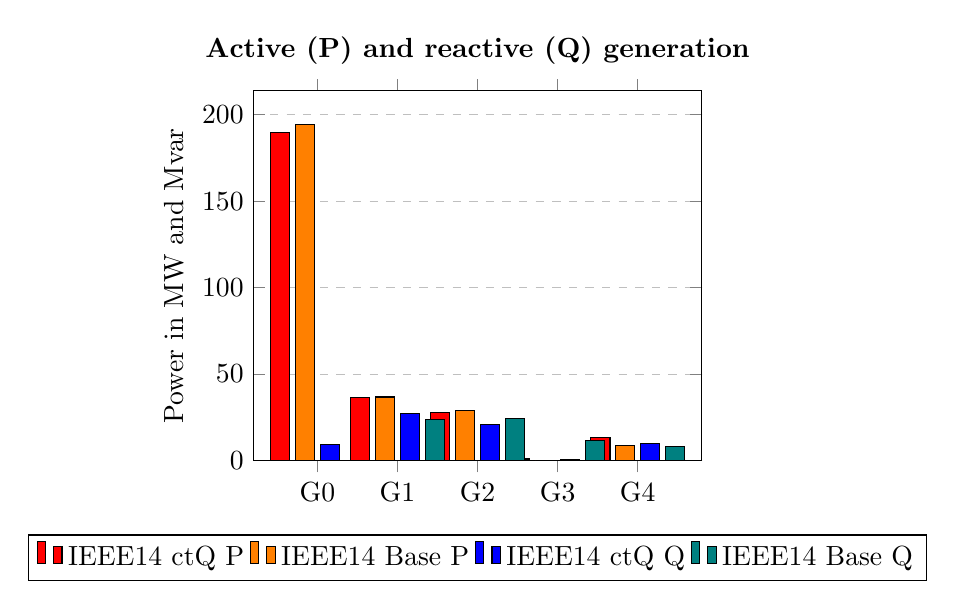
\begin{tikzpicture}
    \begin{axis}[
        title={\textbf{Active (P) and reactive (Q) generation}},
        ybar,
        enlarge x limits=0.2,
        ymin=0,
        width=0.6\textwidth,
        legend style={at={(0.5,-0.2)},
        anchor=north,legend columns=-1},
        ylabel={Power in MW and Mvar},
        symbolic x coords={G0, G1, G2, G3, G4},
        xtick=data,
        nodes near coords align={vertical},
        bar width=7pt,
        ymajorgrids,
        grid style=dashed,
    ]

    \addplot[fill=red] coordinates {(G0,189.83) (G1,36.28) (G2,27.95) (G3,0.85) (G4,13.10)};
    \addplot[fill=orange] coordinates {(G0,194.33) (G1,36.72) (G2,28.74) (G3,0.00) (G4,8.49)};
    \addplot[fill=blue] coordinates {(G0,9.26) (G1,27.21) (G2,20.96) (G3,0.64) (G4,9.83)};
    \addplot[fill=teal] coordinates {(G0,0.01) (G1,23.68) (G2,24.13) (G3,11.54) (G4,8.27)};

    \legend{IEEE14 ctQ P, IEEE14 Base P, IEEE14 ctQ Q, IEEE14 Base Q}
    \end{axis}
    \end{tikzpicture}
    \caption{Generation comparison for the Case IEEE14 with and without reactive control.} 
    \label{fig:ctQ_gen}
\end{figure}

The effect of this constraint can be seen in the cost value of the simulation. Table~\ref{tab:ctQ_cost} shows an increase of around 0.075\% in the cost of operation, which again can be significant in a bigger grid.

\begin{table}[H]
    \centering
    \caption{Cost for Case IEEE14 with Q control.}
    \begin{tabular}{lcc}
    \hline
     & {\textbf{IEEE14 Base}}& {\textbf{IEEE14 ctQ}}\\ \hline\hline
    \textbf{Cost (€/MWh)} & 8081.53 & 8087.82 \\ \hline
    \end{tabular}
    \label{tab:ctQ_cost}
\end{table}

\subsection{DC link and dual price study}

The following study is performed over a small grid with two islands of three buses each. Both of them have the same configuration and elements, but their generators will have different costs profiles as follows:

\begin{equation}
    \begin{split}
        c_{g1.0}(P_{g1.0}) &= 1 \cdot P_{g1.0} + 2 \cdot P_{g1.0}^2 \\
        c_{g1.1}(P_{g1.1}) &= 1 \cdot P_{g1.1} + 3 \cdot P_{g1.1}^2 \\
        c_{g2.0}(P_{g2.0}) &= 1 \cdot P_{g2.0} + 1.5 \cdot P_{g2.0}^2 \\
        c_{g2.1}(P_{g2.1}) &= 1 \cdot P_{g2.1} + 1 \cdot P_{g2.1}^2
    \end{split}
\end{equation}

The grid is firstly tested without interconnection, obtaining the results for each island isolated. Then, a lossless DC link is added between the two islands. In Figure~\ref{fig:island_gen}, 
the comparison between the generation profiles can be seen.

\begin{figure}[H]
    \centering
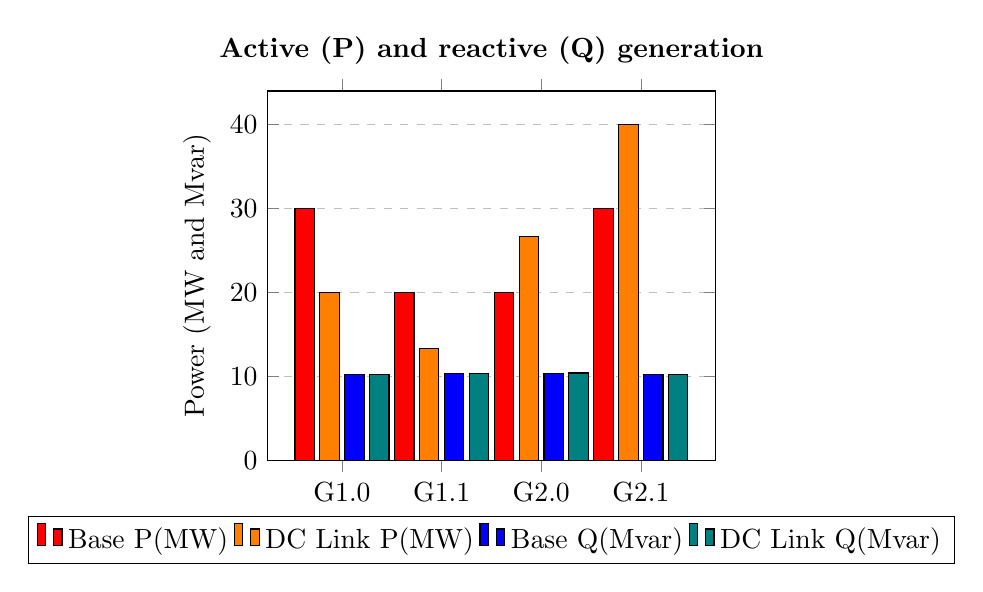
\begin{tikzpicture}
    \begin{axis}[
        title={\textbf{Active (P) and reactive (Q) generation}},
        ybar,
        enlarge x limits=0.25,
        ymin=0,
        width=0.6\textwidth,
        legend style={at={(0.5,-0.15)},
        anchor=north,legend columns=-1},
        ylabel={Power (MW and Mvar)},
        symbolic x coords={G1.0,G1.1,G2.0,G2.1},
        xtick=data,
        nodes near coords align={vertical},
        bar width=7pt,
        ymajorgrids,
        grid style=dashed,
    ]
    \addplot[fill=red] coordinates {(G1.0,30.01) (G1.1,20.01) (G2.0,20.01) (G2.1,30.01)};
    \addplot[fill=orange] coordinates {(G1.0,20.01) (G1.1,13.34) (G2.0,26.67) (G2.1,40.01)};
    \addplot[fill=blue] coordinates {(G1.0,10.26) (G1.1,10.35) (G2.0,10.36) (G2.1,10.25)};
    \addplot[fill=teal] coordinates {(G1.0,10.25) (G1.1,10.39) (G2.0,10.42) (G2.1,10.25)};

    \legend{Base P(MW), DC Link P(MW), Base Q(Mvar), DC Link Q(Mvar)}
    \end{axis}
    \end{tikzpicture}
    \caption{Generation comparison for the island case with and without DC link.}
    \label{fig:island_gen}
\end{figure}

As expected, after both grids are connected, the generators of the second island become prevalent as their prices are lower than the first island, and the power is transferred through this DC link with a total power
of $P_{DC} = 16.67 \text{MW}$. The interconnection has a great impact in the dual price as seen in Figure~\ref{fig:dual_price}.

\begin{figure}[H]
    \centering
    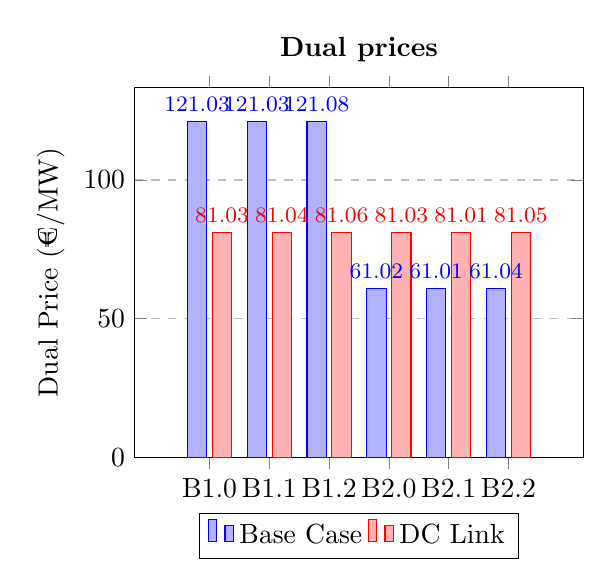
\begin{tikzpicture}
    \begin{axis}[
        title={\textbf{Dual prices}},
        ybar,
        enlarge x limits=0.25,
        ymin=0,
        width=0.6\textwidth,
        legend style={at={(0.5,-0.15)},
        anchor=north,legend columns=-1},
        ylabel={Dual Price (€/MW)},
        symbolic x coords={B1.0,B1.1,B1.2,B2.0,B2.1,B2.2},
        xtick=data,
        nodes near coords,
        nodes near coords align={vertical},
        nodes near coords style={font=\footnotesize},
        bar width=7pt,
        ymajorgrids,
        grid style=dashed,
    ]
    \addplot coordinates {(B1.0,121.027) (B1.1,121.034) (B1.2,121.081) (B2.0,61.017) (B2.1,61.013) (B2.2,61.041)};
    \addplot coordinates {(B1.0,81.025) (B1.1,81.035) (B1.2,81.064) (B2.0,81.025) (B2.1,81.012) (B2.2,81.052)};

    \legend{Base Case, DC Link}
    \end{axis}
    \end{tikzpicture}

    \caption{Dual price comparison for the case with and without DC link.}
    \label{fig:dual_price}
\end{figure}

These results are really important to understand the meaning of the dual price, which for the optimization problem are equal to the value of the equality multipliers associated to the nodal power balance
of each bus. These values indicate the rate of increase in cost that would be caused by demanding an additional infinitesimal amount of power at that bus. 
The following calculations can be done to check which is the cost of generating an additional MW of power per generation, using their cost function and the obtained setpoint from the optimization solution:

\begin{equation}
    \begin{split}
        \frac{\partial c_{g1.0}}{\partial P_{g1.0}}_{Base} & = 1 + 4 \cdot P_{g1.0} = 1 + 4 \cdot 30.0067 = 121.027 \\
        \frac{\partial c_{g1.1}}{\partial P_{g1.1}}_{Base} & = 1 + 6 \cdot P_{g1.1} = 1 + 6 \cdot 20.0056 = 121.034 \\
        \frac{\partial c_{g2.0}}{\partial P_{g2.0}}_{Base} & = 1 + 3 \cdot P_{g2.0} = 1 + 3 \cdot 20.0056 = 61.017 \\
        \frac{\partial c_{g2.1}}{\partial P_{g2.1}}_{Base} & = 1 + 2 \cdot P_{g2.1} = 1 + 2 \cdot 30.0067 = 61.013 \\
    \end{split}
\end{equation}

\begin{equation}
    \begin{split}
        \frac{\partial c_{g1.0}}{\partial P_{g1.0}}_{DC} & = 1 + 4 \cdot P_{g1.0} = 1 + 4 \cdot 20.0062 = 81.025 \\
        \frac{\partial c_{g1.1}}{\partial P_{g1.1}}_{DC} & = 1 + 6 \cdot P_{g1.1} = 1 + 6 \cdot 13.3392 = 81.035 \\
        \frac{\partial c_{g2.0}}{\partial P_{g2.0}}_{DC} & = 1 + 3 \cdot P_{g2.0} = 1 + 3 \cdot 26.6750 = 81.025 \\
        \frac{\partial c_{g2.1}}{\partial P_{g2.1}}_{DC} & = 1 + 2 \cdot P_{g2.1} = 1 + 2 \cdot 40.0057 = 81.012 \\
    \end{split}
\end{equation}

As it can be seen, the values of dual prices for buses with generation are equal to the derivative of those generators connected. For buses with no generation, the price is slightly above since it has to 
account for the additional power injected due to the losses during the power transfer.

Finally, the cost of operation has obviously been reduced after connecting both islands as seen in Table~\ref{tab:DC_cost}. The difference is significant, 
representing a reduction of 11.5\% in the cost of operation. This example shows the economical benefit of having an interconnection to a neighboring grid as the INELFE interconnection between 
Spain and France, apart from the technical benefits in terms of frequency stability, power support during faults, etc. 

\begin{table}[H]
    \centering
    \caption{Costs for Case 2 islands.}
    \begin{tabular}{lcc}
    \hline
     & {\textbf{Base Case 2 islands}}& {\textbf{2 islands + DC link}}\\ \hline\hline
    \textbf{Cost (€/MWh)} & 4602.23 & 4102.12 \\\hline
    \end{tabular}
    \label{tab:DC_cost}
\end{table}


\subsection{Runtime comparison}

Lastly, the execution times of all the cases with each different initialization combination have been measured. All measurements have been reproduced in the same conditions, repeating 5 times each execution to have a larger sample size, although
all the values had low deviation. Results are shown in Figures~\ref{fig:runtime} and~\ref{fig:GBruntime}, separating the larger case for better visualization. 

Overall, the solver seems to be on the same level of performance as Matpower in the cases where a comparison could be made. For smaller cases, Matpower has a slight advantage, while for bigger cases the initialization with a power flow solution
greatly improves the performance of the solver. The slack initialization is slower in most of the cases as expected, but in some cases it performs at the same level as the power flow initialization with no slacks. Bear in mind that this option is not
expected to be used for improved speed, rather for improved convergence.

An important remark to be made is that the power flow execution time is not included in the runtime of the solver, as it is assumed that the user would be able to calculate it once with the built-in power flow
solver, and then use it directly for all the desired studies. Another remark is that this comparison is made with the Python adaptation of Matpower, while the original implementation runs in Matlab/Octave and should be quicker.



\begin{figure}[!htb]
    \centering
    \begin{tikzpicture}
        \begin{axis}[
            ybar,
            ymin=0,
            bar width=7pt,
            width=\textwidth,
            height=0.4\textheight,
            enlarge x limits=0.25,
            legend style={at={(0.5,-0.3)},
                anchor=north,legend columns=-1},
            ylabel={Runtime (s)},
            symbolic x coords={Case 9, IEEE14, IEEE14 Taps, Pegase89, IEEE300, Case GB},
            xtick=data,
            nodes near coords align={vertical},
            x tick label style={rotate=45, anchor=east},
            legend style={font=\footnotesize},
            ymajorgrids,
            grid style=dashed,
        ]

        % MATPOWER
        \addplot[fill=green] coordinates {(Case 9,0.30) (IEEE14,0.39) (IEEE14 Taps, 0) (Pegase89,0.75) (IEEE300,1.38)};
        
        % PowerFlow
        \addplot[fill=red] coordinates {(Case 9,0.52) (IEEE14,0.42) (IEEE14 Taps,0.80) (Pegase89,0.66) (IEEE300,0.93)};
        
        % No PowerFlow
        \addplot[fill=orange] coordinates {(Case 9,0.50) (IEEE14,0.51) (IEEE14 Taps,0.83) (Pegase89,1.02) (IEEE300,1.03)};
        
        % PowerFlow + slacks
        \addplot[fill=blue] coordinates {(Case 9,0.65) (IEEE14,0.64) (IEEE14 Taps,0.92) (Pegase89,0.64) (IEEE300,1.60)};
        
        % No PowerFlow + slacks
        \addplot[fill=cyan] coordinates {(Case 9,0.65) (IEEE14,0.67) (IEEE14 Taps,0.78) (Pegase89,2.18) (IEEE300,1.22)};

        \legend{MATPOWER,PowerFlow,No PowerFlow,PowerFlow + slacks,No PowerFlow + slacks}
        \end{axis}
    \end{tikzpicture}
    \caption{Runtime comparison for different cases.}
    \label{fig:runtime}
\end{figure}


\begin{figure}[!htb]
    \centering
    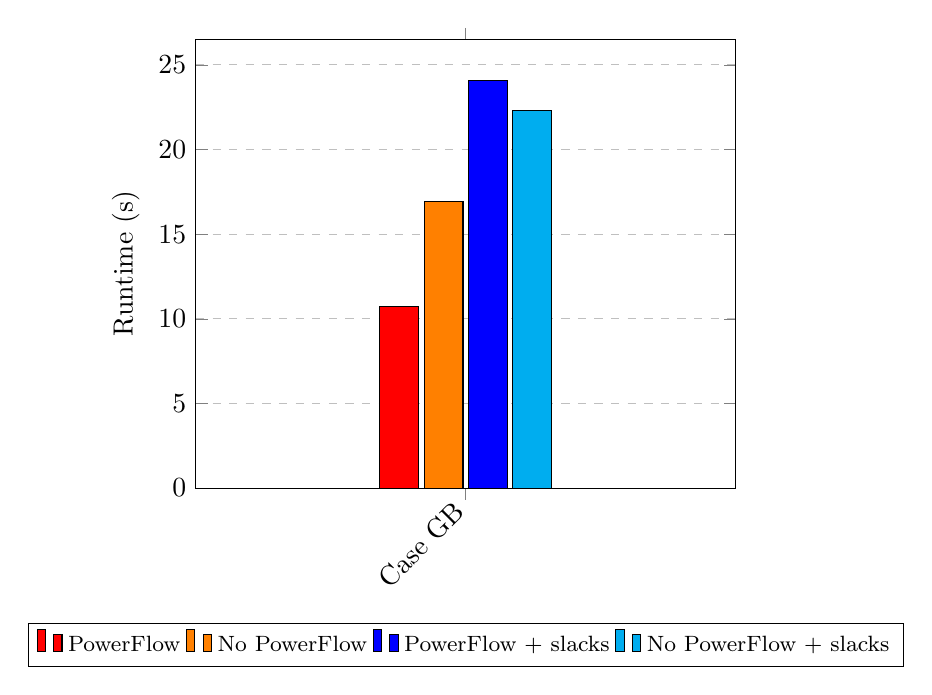
\begin{tikzpicture}
        \begin{axis}[
            ybar,
            enlarge x limits=0.5,
            ymin=0,
            bar width=14pt,
            legend style={at={(0.5,-0.3)},
            anchor=north,legend columns=-1},
            ylabel={Runtime (s)},
            symbolic x coords={Case GB},
            xtick=data,
            nodes near coords align={vertical},
            x tick label style={rotate=45, anchor=east},
            legend style={font=\footnotesize},
            ymajorgrids,
            grid style=dashed,
        ]
        % PowerFlow
        \addplot[fill=red] coordinates {(Case GB,10.75)};
        
        % No PowerFlow
        \addplot[fill=orange] coordinates {(Case GB,16.92)};
        
        % PowerFlow + slacks
        \addplot[fill=blue] coordinates {(Case GB,24.08)};
        
        % No PowerFlow + slacks
        \addplot[fill=cyan] coordinates {(Case GB,22.30)};

        \legend{PowerFlow,No PowerFlow,PowerFlow + slacks,No PowerFlow + slacks}
        \end{axis}
    \end{tikzpicture}
    \caption{Runtime comparison for the GB case.}
    \label{fig:GBruntime}
\end{figure}

\newpage

\section{Conclusion}\label{Conclusion}

\subsection{Further Work}



\begin{itemize}
    \item -

\end{itemize}
\newpage


\section*{Acknowledgments}\label{acknow} 
\addcontentsline{toc}{section}{Acknowledgments}
I want to thank Marc Cheah and Josep Fanals, my thesis supervisors from UPC and eRoots respectively, for the opportunity to develop this project in collaboration with Redeia and for their guidance and support through the process.
I'd also like to thank Santiago Peñate for his help in developing the tool and integrating it in GridCal in collaboration with Josep and me.

\appendix
\cleardoublepage
\section{Environmental, Social, and Gender Impact}

\section{Environmental impact}

An environmental contribution of this work lies in its support for energy efficiency and the 
ongoing energy transition. The developed framework contributes to the optimal operation and planning
of power systems with high shares of renewable generation. Stability analysis allows network operators to 
safely integrate variable renewable sources such as wind and solar while maintaining system reliability. 
This, in turn, facilitates higher utilization of clean energy resources and reduces curtailment, 
leading to a more efficient use of installed capacity and a measurable reduction in carbon emissions. 
In a broader context, the development of robust and open simulation tools is essential to achieving global 
decarbonisation objectives and ensuring a stable, sustainable transition towards a low-carbon energy system \cite{IEA2024Transition}.

Although the present work involves primarily computational and simulation tasks rather than physical infrastructure,
it nonetheless carries meaningful environmental implications. Advanced RMS and EMT tools aid in the integration of 
renewable energy sources by improving the predictability and security of grid behavior, thereby helping reduce
reliance on fossil fuel backup plants and associated greenhouse gas emissions\cite{XiongParaEMT2024}. 
The trade-off between simulation fidelity and computational cost is also well documented; for example, Yan et al.\ examine
the impact of different numerical integration schemes on simulation accuracy and efficiency \cite{YanCompEff2025}. 
Minimizing computational energy consumption through algorithmic optimization is thus a relevant concern.

Moreover, the promotion of open-source platforms in power system research enhances resource efficiency by reducing 
duplicated development efforts and enabling community-driven innovation. The use of openly shared modeling libraries 
accelerates progress and lowers barriers to entry\cite{TesfatsionOpenSource}. By providing validated simulation tools, 
this work contributes to more sustainable and cost-effective grid planning, potentially reducing the environmental 
footprint of energy infrastructure expansion.

On the other side, the actual footprint of the project development can be computed as kg of $CO_2$ equivalent emitted
to the atmosphere. This study estimates the direct environmental footprint accounting for the
electricity consumed by the computer and monitor, the corresponding share of HVAC energy use and the amortized embodied 
emissions of the electronic equipment. 
The calculation considers a five-month period (September to January), with a working schedule of eight hours per day, Monday to Friday. 
This corresponds to approximately $22$~weeks~$ \cdot $~5~days/week~$ \cdot $~8~h/day~$\approx~880$~hours.

The working environment corresponds to a small office space in the center of Barcelona, shared by approximately 20 occupants. In order to simplify the 
study, the following assumptions are done:

\begin{itemize}
    \item Only the energy used by the laptop and the monitor are considered.
    \item The kg of $CO_2$ equivalent emitted by the manufacturing and transportation of the laptop and monitor are considered. The office equipment is not considered.
    \item Only the energy consumption due to HVAC in the office is considered due to its high contribution to energy consumption in the office.
\end{itemize}


For the Laptop embodied emissions Circular Computing \cite{CircularComputing2022} proposes 331~kg\,CO$_2$eq/device accounting for manufacturing,
transport and 4 first years of use. According to their calculations, manufacturing and transport accounts by approximately 90\% of those emissions.
For the monitor, a standard monitor has been selected. HP sustainability report \cite{HP2021MonitorLCA} states that 210~kg\,CO$_2$eq/device 
are emitted during manufacturing, transport, use and end of life. Manufacturing, transport and end of life account for a 47\% of those emissions.
According to l'Institut Català de l'Energia (ICAEN) \cite{ICAEN}, the recommended average HVAC energy consumption in an office building is 140~kWh/m$^2$~year. 
Scaling this consumption to an average of 5m$^2$ per person in a office and 260 working days a year the resulting energy consumption is 
0,299 kWh/hour~person. For the allocation factor of the laptop and monitor, 5 years of lifespan are assumed.

All parameters used are summarized in Table~\ref{tab:co2_inputs_full}.

\begin{table}[H]
\centering
\caption{Emission factors and embodied carbon data used in the estimation.}
\label{tab:co2_inputs_full}
\renewcommand{\arraystretch}{1.15}
\small
\begin{tabular}{|l|c|c|l|}
\hline
\textbf{Source / Component} & \textbf{Value} & \textbf{Unit} & \textbf{Reference} \\ 
\hline
Electricity emission factor (Spain, 2023) & 0,26 & kg\,CO$_2$eq/kWh & \cite{Gencat2023FactorsEmissio} \\ 
Laptop embodied emissions (manufacturing) & 297,9 & kg\,CO$_2$eq/device & \cite{CircularComputing2022} \\ 
Monitor embodied emissions (manufacturing) & 94,47 & kg\,CO$_2$eq/device & \cite{HP2021MonitorLCA} \\ 
Average laptop power draw & 45 & W & \cite{AsusVivabook} \\ 
Average monitor power draw & 37 & W & \cite{AOC} \\ 
HVAC energy use per occupant (shared office) & 0,299 & kWh/h~pers & \cite{ICAEN} \\ 
Allocation factor laptop and monitor & 0.084 & -- & assumed \\ 
\hline
\end{tabular}
\end{table}

The total electricity consumption during the five-month period can be expressed as:

\begin{equation}
E_{total} = E_{PC+monitor}  + E_{HVAC}~[kWh]
\end{equation}
where:

\begin{equation}
E_{PC+monitor} = (P_L~W + P_M ~W) \cdot  \frac{880~h}{1000~W/kW} = 72,16 kWh
\end{equation}
\begin{equation}
E_{HVAC} = 0,299~kWh/h \cdot 880~h = 263,25~kWh
\end{equation}

Corresponding to a total of 87,206 kg of CO$_2$eq due to energy consumption.

The allocation contribution of the LCA for the laptop and monitor correspond to a total of $(297,9 + 94,47)$~kg~CO$_2$eq $\cdot 0,084 = 32,959$~kg~CO$_2$eq.

The total emissions are 120,165 kg of CO$_2$eq. Table \ref{tab:contribution_CO2} summarizes the contribution of each element to the total 

\begin{table}[H]
\centering
\caption{Estimated carbon footprint of the thesis work including HVAC, lighting, and office equipment.}
\label{tab:contribution_CO2}
\renewcommand{\arraystretch}{1.15}
\small
\begin{tabular}{|l|c|c|}
\hline
\textbf{Component} & \textbf{kg\,CO$_2$eq emissions } & \textbf{Contribution} \\ 
\hline
Laptop + monitor operation & $18,761$ & $15,613~\%$ \\ 
HVAC energy consumption & $68,444$ & $56,958~\%$ \\ 
Allocated embodied emissions (laptop + monitor) & $32,959$ & $27,428~\%$ \\ 
\hline
\textbf{Total estimated footprint} & \textbf{120,165} &  \\ 
\hline
\end{tabular}
\end{table}

Results conclude that the main contribution to the project development global emissions are due to the office HVAC being the 56,95\% of 
the total equivalent CO$_2$ emissions. Regarding the laptop and monitor it is seen how the manufacturing and transporting contribution
is much higher than the operation itself, highlighting the importance of Life Cycle Assessments on the environmental assessments.

To contextualize the estimated footprint of this work, it is useful to compare it with reference studies on greenhouse gas emissions in office environments. 
According to the European Environment Agency, the annual emissions associated with a standard office workplace in 
Europe (including HVAC, lighting, equipment, and commuting) are between 1500 and 2000~kg\,CO$_2$eq per employee \cite{EEA2021OfficeEnergy}. The corresponding contribution
of 5 months is  between 625 and 833~kg\,CO$_2$eq. As noted, in this study the EEA considers also the commuting to work. Circular Ecology \cite{CircularEcology} states that, in Europe. only 53\%
of the emissions of going to work in an office account for the office itself meaning 47\% of the emissions correspond to commuting. Applying this percentage
the average office emissions(including HVAC, lighting, equipment) in Europe are between 331,250 and 441,677~kg\,CO$_2$eq.

In comparison, the total estimated footprint of approximately 120~kg\,CO$_2$eq for this thesis project is lower than the studies stated in the previous paragraph.
It is to be considered that the EEA study considers both lightning and equipment while this study does not. Moreover, the average energy consumption in Europe is
higher than in Spain so this result may be affected. Therefore, the result is considered correct and highlights the importance of energy-efficient habits.

\section{Gender and social impact}

TO CHECK!!

Beyond technical contributions, this project supports broader social goals through the promotion of inclusive and accessible tools. 
Open-source frameworks for power system analysis democratize advanced engineering capabilities, enabling participation from researchers 
and engineers in diverse regions and institutions. For instance, the development of open and transparent electricity network 
models demonstrates how access to modeling tools can empower under-resourced communities \cite{KirliPyPSA2021}. Open-source frameworks
support the idea that knowledgment must be a social right and accessible for everybody.

From a gender perspective, power systems engineering remains dominated by men in many contexts. Disseminating open methodologies 
and encouraging diverse collaboration may help widen participation of underrepresented groups in STEM fields. 

Finally, improving the reliability, stability, and efficiency of power systems has direct social benefits: fewer outages, better access to electricity, 
and more resilient grids that support sustainable development goals.  



\cleardoublepage
\section{Time Planning}
Figure \ref{fig:gantt} shows the temporal evolution of the various tasks that have constituted the project.
\begin{figure}[H]
  \centering
  \resizebox{\textwidth}{!}{
  
  \begin{ganttchart}[y unit title=0.6cm,
  y unit chart=0.7cm,
  vgrid,hgrid, 
  title label anchor/.style={below=-1.6ex},
  title left shift=.05,
  title right shift=-.05,
  title height=1,
  progress label text={},
  bar height=0.5,
  group right shift=0,
  group top shift=.6,
  group height=.3]{1}{32}
  %labels
  \gantttitle{2023}{16} 
  \gantttitle{2024}{16}\\
  \gantttitle{September}{4} 
  \gantttitle{October}{4} 
  \gantttitle{November}{4} 
  \gantttitle{December}{4} 
  \gantttitle{January}{4} 
  \gantttitle{February}{4} 
  \gantttitle{March}{4}
  \gantttitle{April}{4} \\
  %tasks
  \ganttbar{Literature review}{3}{6} \\
  \ganttbar{Model development}{7}{10} \\
  \ganttbar{Basic solver development}{11}{16} \\
  \ganttbar{GridCal integration}{15}{16} \\
  \ganttbar{Addition of new fatures}{17}{22} \\
  \ganttbar{Benchmarking}{23}{26} \\
  \ganttbar{Documentation}{25}{32} \\
  
  %relations 
  \ganttlink{elem0}{elem1} 
  \ganttlink{elem0}{elem4} 
  \ganttlink{elem1}{elem4} 
  \ganttlink{elem2}{elem4}
  \ganttlink{elem2}{elem3} 
  \ganttlink{elem3}{elem4} 
  \ganttlink{elem4}{elem5} 
  \ganttlink{elem5}{elem6} 
  \end{ganttchart}
  }
  \caption{Gantt Chart of the project.}
  \label{fig:gantt}
\end{figure}

\cleardoublepage
\section{Budget}


The complete costs are detailed in Table~\ref{tab:equip}.

-	Les hores emprades per la realització del treball (les corresponents als crèdits del TFE). Millor 
si estan separades per les tasques executades segons la planificació. En una primera aproximació podeu considerar
 que una de les vostres hores es paga a 15 €/h.
-	Les despeses operatives: electricitat, calefacció, aigua o telefonia. Sumeu la part proporcional dels termes fixos.
 També tingueu en compte els viatges, les despeses d'oficina i d'altres.
-	Les despeses experimentals: materials, aigua, electricitat, combustibles, llicències, llibres.
-	Si és el cas, amortització dels equips. Considereu que un PC s'amortitza linealment en 5 anys i un telèfon mòbil en 3 anys.
-	Serveis abonats per obtenir algunes dades (per exemple d'un servei de microscòpia electrònica, encara que no ho hagi pagat l'estudiant).
-	I totes aquelles que haurien de constar si el treball fos realista i s'hagués de facturar. 


\begin{table}[!htb]\centering
	\caption{Total Costs.}
	\begin{tabular}{ccc|c}
		\hline
		\textbf{Concept} & \textbf{Unit cost (\texteuro/h)} & \textbf{Quantity (h)} & \textbf{Total (\texteuro)} \\
		\hline
		\hline
		Development engineer & 25.00 & 1,040 & 26,000.00 \\ 
		Supervisor & 30.00 & 260 & 7,800.00 \\
		\hline
		\textbf{Total} & & & 33,800.00 \\
		\hline
	\end{tabular}
	\label{tab:equip}
\end{table}



%bibliography
\cleardoublepage
%\renewcommand\refname{Bibliography}
%pdf\addcontentsline{toc}{section}{Bibliography}
\printbibliography

\end{document}

